% This work is licensed under the Creative Commons
% Attribution-NonCommercial-ShareAlike 4.0 International License. To view a copy
% of this license, visit http://creativecommons.org/licenses/by-nc-sa/4.0/ or
% send a letter to Creative Commons, PO Box 1866, Mountain View, CA 94042, USA.

%%%%%%%%%%%%%%%%%%%%%%%%%%%%%%%%%%%%%%%%%%%%%%
% Dies ist nur eine Vorlage und soll die künstlerische Freiheit des Autors einer Mitschrift in keiner Weise schmälern.
% Der Inhalt dieser Vorlage soll eher Möglichkeiten anbieten und bewährte Lösungswege aufzeigen.
% Wichtige Dinge sind aktuell enthalten, optionale Dinge sind auskommentiert.
%%%%%%%%%%%%%%%%%%%%%%%%%%%%%%%%%%%%%%%%%%%%%%

\documentclass[]{scrreprt}

\newcommand{\directoryPrefix}{../latex/} 
\input{\directoryPrefix packages}
%\input{\directoryPrefix counters} % section counter benutzt römische Zahlen
\input{\directoryPrefix theoremenvironments}
\input{\directoryPrefix font}
\input{\directoryPrefix commands}
%\input{\directoryPrefix commands_Willi}
%% This work is licensed under the Creative Commons
% Attribution-NonCommercial-ShareAlike 4.0 International License. To view a copy
% of this license, visit http://creativecommons.org/licenses/by-nc-sa/4.0/ or
% send a letter to Creative Commons, PO Box 1866, Mountain View, CA 94042, USA.

\renewcommand{\K}{\mathcal{K}} % Formelmenge % lokale Commands und packages werden auch ausgelagert. Lokal bedeutet nur diese Vorlesung betreffend.

\makeindex % erstellt Stichwortverzeichnis
\setlength{\parindent}{0px} % verhindert das Einrücken eines Absatzes bei einer leeren Codezeile.
%\renewcommand{\thesection}{\arabic{section}} % nützlich, falls es keine Chapter, sondern nur sections gibt.

\title{
	Vorlesung\\
	Wissenschaftliches Rechnen\\
	Fortgeschrittene Aspekte
}
%\subject{Thema}
\subtitle{Sommersemester 2019}
\author{
	Vorlesung:  Dr. Marco Salvalaglio \& Prof. Dr. Axel Voigt\\
	Mitschrift: Robert Walter
}
\date{\today}
\publishers{\url{https://github.com/LostInDarkMath/MatheMaster}}
%\dedication{Widmung}

\begin{document}
	%\begin{hack}: fix overfull hbox warning caused by \tableofcontents when exceeding 100 pages	
	\makeatletter
  	\renewcommand{\@pnumwidth}{2em}
  	%\renewcommand{\@tocrmarg}{3em} % currently unnecessary
  	\makeatother
  	%\end{hack}
  	
  	%\selectlanguage{english}
  	
	\pagenumbering{gobble}	% disable pagenumbering
	\maketitle
	%\epigraph{Hier steht eine Lebensweisheit.}{\textit{Der Admin}}
	%\newpage
	\doclicenseThis
	\tableofcontents
	\pagenumbering{arabic}	% enable pagenumbering
	
	%\addchap{Hauptüberschrift} % sinnvoll in Kombination mit Zeile 15
	% !TEX root = SCCOMP.tex
% This work is licensed under the Creative Commons
% Attribution-NonCommercial-ShareAlike 4.0 International License. To view a copy
% of this license, visit http://creativecommons.org/licenses/by-nc-sa/4.0/ or
% send a letter to Creative Commons, PO Box 1866, Mountain View, CA 94042, USA.

\chapter{Large Sparse Linear Systems}
\section{Model problems and discretization}%
\label{sec:Modelproblems and discretization}


\begin{equation}\label{eq:eq_1}\tag{1}
	\frac{\partial^2 u}{\partial x_1^2} + \frac{\partial^2 u}{\partial x_2^2} =: \laplace u = f(x) 
\end{equation}
with $\Omega \subset \R^2$ bounded, open domain and 
$ x =
\begin{pmatrix}
x_1 \\
x_2
\end{pmatrix}
\in \Omega$
\begin{figure}[H]
	\center
\begin{tikzpicture}[scale=3]
		
		\def \xone{0};
		\def \yone{0};		
		% draw coordinate system
		\coordinate (A) at (\xone,\yone);
		
		\draw[->] (A) -- ++(0,1);
		\draw[->] (A) -- ++(1,0);
		\draw[->] (A) ++(0.9,0.5) -- ++(0.5,0);

		% a circle is easier to draw than another object
        \draw (A) ++(0.5,0.5) circle (0.4cm);
        
        \fill[black,font=\footnotesize] (A) ++(1,0) node[below] {$x_{1}$}
										(A) ++(0,1) node[left] {$x_{2}$}
										(A) ++(1.4,0.5) node[below] {$n$};
                                        
\end{tikzpicture}

\caption{example $\Omega$,  $n$   outer normal on $\partial \Omega$}
\label{first picture}
\end{figure}

n outer normal on $\partial \Omega$
with boundary conditions
\[
\alpha u + \beta \frac{\partial u}{\partial n} = g \qquad \text{ on } \partial \Omega
.\] 

If \begin{itemize}
	\item $ \beta = 0$ and $\alpha=0$, we get a Dirichlet problem.
	\item  $\beta \neq 0$ and $ \alpha = 0$, we get a general Neumann problem.
	\item $\beta = 1$ and $\alpha = 0$, we have
		\begin{enumerate}
			\item Since $u = \text{const}$ solves \href{eq:eq_1}{(1)} 
				for $f=0 \text{ and } g = 0$, the solution to \href{eq:eq_1}{(1)} is unique up to a constant
			\item Integrating \href{eq:eq_1}{(1)} over $\Omega$ and Green's formula yield
				\[
				- \int_{\partial\Omega} \frac{\partial u}{\partial n} = - \int_{\Omega} \laplace u = \int_{\Omega} f
				.\] 
				This means, we get a compatibility condition
				\[
				\int_{\partial \Omega} g + \int_{\Omega}f = 0
				.\] 
		\end{enumerate}
\end{itemize} 

Another variant of \href{eq:eq_1}{(1)} is
\[
	Lu := \nabla(A\nabla u)
.\] 
where A is a positive definite matrix.

\begin{equation} \label{eq:eq_2}\tag{2}
LU = f \qquad \in \Omega \text{ + boundary condition}
\end{equation}

\section{Discretization with finite differences}%
\label{sec:Discretization with finite differences}

The basic idea is:

\begin{itemize}
	\item local approximation of partial derivatives
	\item derived by low order Taylor series
\end{itemize}

\begin{itemize}
	\item \underline{(1D-case):} 
		\[
			u'(x) \approx \frac{u(x+h)-u(x)}{h} = \delta^{+}u(x) \qquad \text{(forward difference)}
		.\] 
		For functions $u \in C^{4}$ in a neighbourhood of $x$, we get by Taylor's formula:
		\begin{equation} \label{eq:eq_3} \tag{$\ast$}
			u(x+h) = u(x) + h u'(x) + \frac{h^{2}}{2} u''(x) + \frac{h^{3}}{6}u'''(x) + \frac{h^{4}}{24}u''''(\xi_{+})	
		\end{equation}
		for some $\xi_{+} \in (x, x+h)$. Rearranging the equation gives
		\[
			u'(x) = \frac{u(x+h)-u(x)}{h}-\frac{h}{2}u''(x) + \O(h^{2})
		.\] 
		Now we plug this in in \href{eq:eq_4}{($\ast$)} and replace $h$ by $-h$ to get
		\begin{equation} \label{eq:eq_4} \tag{$\ast \ast$}
			u(x-h) = u(x) - hu'(x) + \frac{h^{2}}{2}u''(x)- \frac{h^{3}}{6} u'''(x) + \frac{h^{4}}{24}u''''(\xi _{-})
		\end{equation}
		For some appropriate $\xi _{-} \in (x-h, x)$.
		Adding up \href{eq:eq_3}{($\ast$)} and \href{eq:eq_4}{($\ast \ast)$} yields
		\[
			u''(x)= \frac{u(x+h) - 2u(x) + u(x-h)}{h^{2}} + \frac{h^{2}}{12}u''''(\xi )
		.\] for some $\xi  \in [\xi _{-}, \xi _{+}]$

		This is called the central difference approximation of the second order derivative.
		
		Let
		\[
			u'(x) \approx \frac{u(x)-u(x-h)}{h} = \delta^{-}u(x) \qquad \text{(backward difference)}
		.\] Then $u''(x) \approx \delta^{-}\delta^{+}u(x)$.

		For the elliptic operator $L:=\partial_{x} \Big(a(x)\partial_{x}\Big)$ we get a second order accurate formula by evaluating $a(x)$ inside the intervals $(x-h, x)$ and $(x, x+h)$
		\begin{align*}
			\partial_{x}(a(x) \partial_{x}u) &=
			\delta^{+}\Big(a(x- \frac{h}{2}) \delta^{-} u\Big) + \O(h^{2}) \\
											 &\approx \frac{a(x+\frac{h}{2})\Big(u(x+h)-u(x)\Big)-a(x-\frac{h}{2})\Big(u(x)-u(x-h)\Big)}{h^{2}}
		\end{align*}
		with $a(x \pm \frac{h}{2})$ either evaluated directly or by the average
		\[
			a(x \pm \frac{h}{2}) \approx \frac{1}{2}\Big(a(x \pm h) - a(x)\Big)
		.\] 
		
	\item \underline{(2D \& 3D cases):} 
		The laplacian is the sum of all second derivatives
		\[
			\laplace = \partial x_1^2 + \partial x_2^2 (+\partial x_3^2)
		.\] 
		With (possibly) different step width $h$ in each coordinate direction we get
		\begin{align*}
			\laplace u(x) &\approx \frac{u(x_1 + h_1, x_2) - 2u(x_1, x_2) + u(x_1 -h_1, x_2)}{h_1^2}\\
						  &+ \frac{u(x_1, x_2 + h_2) - 2u(x_1, x_2) + u(x_1, x_2 -h_2)}{h_2^2}
		\end{align*}
		but for $h_1 = h_2 = h$ we get
		\begin{align*}
			&\laplace u(x) \approx\\ 
			&\frac{1}{h^2}\left[u(x_1+ h, x_2) + u(x_1-h, x_2) + u(x_1, x_2 -h) + u(x_1, x_2 -h) -4u(x_1, x_2)\right].
		\end{align*}
		Denoting the forward/backward difference formulas
		in the direction i by $\delta_{i}^{+}$ and $\delta_{i}^{-}$ we can write
		\[
			\laplace u(x) \approx \sum_{i=1}^{2}{\delta_{i}^{+}\delta_{i}^{-}u(x)}=:\laplace_{h}^{(5)}u(x)
		.\] 
		The formula can be sketched as a stencil, the so called " 5-point stencil "
		\tikzset
{
	treenode/.style = {circle, draw=black!60, fill=white!40, very thick, minimum size=6mm}
}

\begin{figure}[H]
	\center

	\begin{tikzpicture}%[level/.style={sibling distance = 2cm/#1, level distance = 3cm}]
	
	\def \xone{0};
	\def \yone{0};
	
	\coordinate (root) at (\xone ,\yone);
	\draw (root) ++ (-1,0) -- ++(2,0);
	\draw (root) ++ (0,-1) -- ++(0,2);

	%draw nodes
	\node [treenode] at (root) {-4};
	\node [treenode] at (root) ++ (-1,0) {1};
	\node [treenode] at (root) ++ (1,0) {1};
	\node [treenode] at (root) ++ (0,1) {1};
	\node [treenode] at (root) ++ (0,-1) {1};

		
	\end{tikzpicture}
	
\caption{5-point stencil (second order accurate)}
\label{five_point}
\end{figure}

		where the values in the nodes correspond to the coefficients in the formula.
		Other possible stencils are:
		\begin{itemize}
			\item rotated 5-point-stencil, $2^{\text{nd}}$ order accurate
				\begin{figure}[H]
	\center

	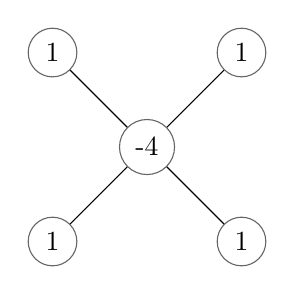
\begin{tikzpicture}

	\def \xone{0};
	\def \yone{0};
	\def \h{1.2}	

	\coordinate (M) at (\xone ,\yone);
	\coordinate (LU) at (\xone-\h ,\yone-\h);
	\coordinate (RU) at (\xone+\h ,\yone-\h);
	\coordinate (LO) at (\xone-\h ,\yone+\h);
	\coordinate (RO) at (\xone+\h ,\yone+\h);
	\draw (LU) -- (RO);
	\draw (RU) -- (LO);

	%draw nodes
	\node[circle,draw=black!60, fill=white!40] at (M) {-4};
	\node[circle,draw=black!60, fill=white!40] at (LO) {1};
	\node[circle,draw=black!60, fill=white!40] at (RO) {1};
	\node[circle,draw=black!60, fill=white!40] at (LU) {1};
	\node[circle,draw=black!60, fill=white!40] at (RU) {1};

		
	\end{tikzpicture}
\caption{rotated 5-point stencil}
\label{five_point_rot}
	
\end{figure}

			\item 9-point-stencil,  $2^{\text{nd}}$ order accurate and even $6^{\text{th}}$ order accurate for harmonic functions
				\begin{figure}[H]
	\center

	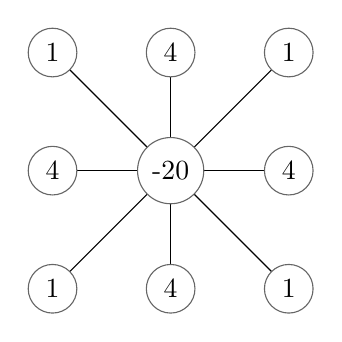
\begin{tikzpicture}
	
	\def \xone{0};
	\def \yone{0};
	\def \h{1.5}	

	\coordinate (M) at (\xone ,\yone);
	\coordinate (L) at (\xone-\h ,\yone);
	\coordinate (R) at (\xone+\h ,\yone);
	\coordinate (O) at (\xone ,\yone+\h);
	\coordinate (LU) at (\xone-\h ,\yone-\h);
	\coordinate (RU) at (\xone+\h ,\yone-\h);
	\coordinate (LO) at (\xone-\h ,\yone+\h);
	\coordinate (RO) at (\xone+\h ,\yone+\h);
	\coordinate (U) at (\xone ,\yone-\h);

	\draw (L) -- (R);
	\draw (U) -- (O);
	\draw (LU) -- (RO);
	\draw (RU) -- (LO);

	%draw nodes
	\node[circle,draw=black!60, fill=white!40] at (M) {-20};
	\node[circle,draw=black!60, fill=white!40] at (L) {4};
	\node[circle,draw=black!60, fill=white!40] at (R) {4};
	\node[circle,draw=black!60, fill=white!40] at (O) {4};
	\node[circle,draw=black!60, fill=white!40] at (U) {4};

	%draw diagonal nodes
	\node[circle,draw=black!60, fill=white!40] at (LO) {1};
	\node[circle,draw=black!60, fill=white!40] at (RO) {1};
	\node[circle,draw=black!60, fill=white!40] at (LU) {1};
	\node[circle,draw=black!60, fill=white!40] at (RU) {1};

	
	\end{tikzpicture}
	\caption{9-point stencil}
\label{nine_point}
	
\end{figure}

		\end{itemize}
\end{itemize}

\subsection{Finite difference on a grid}%
\label{sec:Finite difference on a grid}
Let $\Omega =(0, X_{E}) \times (0,Y_{E})$ and subdivide each interval into $N_{x}+1 / N_{y} + 1$ subintervals.

\[
\left.
	\begin{array}{c}
	N_{x} = 1 \\
	N_{y} = 2
\end{array}
\right\} \qquad
h_{x} = \frac{x_{E}}{N_{x}+1}, \quad h_{y}= \frac{y_{E}}{N_{y}+1}
.\] 

\begin{figure}[H]
	\center
\begin{tikzpicture}[scale=3]
		
		\def \xone{0};
		\def \yone{0};		
		% draw coordinate system
		\coordinate (A) at (\xone,\yone);
		
		\draw[\to] (A) -- ++(0,1);
		\draw[\to] (A) -- ++(1,0);
		\draw (A) ++(0.5,0) -- ++ (0,1);
		\draw (A) ++(1,0) -- ++ (0,1) -- ++(-1,0);
		\draw (A) ++(0,0.333) -- ++ (1,0);
		\draw (A) ++(0,0.666) -- ++ (1,0);
		\draw[red!60] (A) -- (A) ++ (0,0.333);
		\draw[blue!60] (A) -- (A) ++ (0.5,0);

        \fill[black,font=\footnotesize] (A)  ++(1,0) node[under] {$x_{E}$}
										(A)  ++(0,1) node[left] {$y_{E}$}
										(A)  ++(0.25,0) node[under] {$h_{x}$}
										(A)  ++(0,0.1666) node[left] {$h_{y}$};
                                        
\end{tikzpicture}

\caption{Visualization of Grid}
\label{example_grid}
\end{figure}

Each node (vertex) in this grid is assigned an index tuple
\[
	(x,y) = (ih_{x}, jh_{y}) \stackeq{\wedge} (i,j)
.\] 
for $i \in \{0,1, \ldots , N_{x}+1\}, j \in  \{0,1, \ldots , N_{y}+1\}$

We denote the value at the node $(i,j)$ by
\[
	u(x,y)=u(ih_{x},jh_{y})=:u_{i,j}
.\] 
This results in the discrete Laplace operator $(h=h_{x}=h_{y})$
\[
	\laplace_{h}^{(5)}u_{i,j}=\frac{1}{2}(u_{i+1,j}+u_{i-1,j} +u_{i,j+1}+ u_{i,j-1} - 4u_{i,j})
.\]

\newpage
\subsection{Node ordering}%
\label{sec:Node ordering}
To form a linear system, the nodes $(i,j)$ have to be numbered consecutively, i.e. we have to use a map
\[
	l\colon \N^{d} \rightarrow \N
.\] 

Examples:

\begin{enumerate}[label=\alph{enumi})]
	\item  Lexicographical ordering
		\[
			l(i,j) = j \cdot (N_{x} + 2) + i 
			\quad\text{ or }\quad
			l(i,j) = i \cdot (N_{y} + 2) + j
		.\] 

		\begin{figure}[ht!]
			\begin{center}
				

\tikzset{every picture/.style={line width=0.75pt}} %set default line width to 0.75pt        

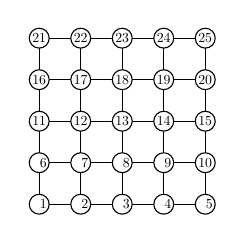
\begin{tikzpicture}[x=0.75pt,y=0.75pt,yscale=-1,xscale=1]
%uncomment if require: \path (0,214); %set diagram left start at 0, and has height of 214

%Shape: Grid [id:dp20427001490833852] 
\draw  [draw opacity=0][fill={rgb, 255:red, 255; green, 255; blue, 255 }  ,fill opacity=1 ] (289.5,62) -- (369.67,62) -- (369.67,142.5) -- (289.5,142.5) -- cycle ; \draw   (289.5,62) -- (289.5,142.5)(309.5,62) -- (309.5,142.5)(329.5,62) -- (329.5,142.5)(349.5,62) -- (349.5,142.5)(369.5,62) -- (369.5,142.5) ; \draw   (289.5,62) -- (369.67,62)(289.5,82) -- (369.67,82)(289.5,102) -- (369.67,102)(289.5,122) -- (369.67,122)(289.5,142) -- (369.67,142) ; \draw    ;
%Shape: Circle [id:dp7961893048519293] 
\draw  [fill={rgb, 255:red, 255; green, 255; blue, 255 }  ,fill opacity=1 ] (284.71,142) .. controls (284.71,139.35) and (286.85,137.21) .. (289.5,137.21) .. controls (292.15,137.21) and (294.29,139.35) .. (294.29,142) .. controls (294.29,144.65) and (292.15,146.79) .. (289.5,146.79) .. controls (286.85,146.79) and (284.71,144.65) .. (284.71,142) -- cycle ;
%Shape: Circle [id:dp11966537247793707] 
\draw  [fill={rgb, 255:red, 255; green, 255; blue, 255 }  ,fill opacity=1 ] (304.71,142) .. controls (304.71,139.35) and (306.85,137.21) .. (309.5,137.21) .. controls (312.15,137.21) and (314.29,139.35) .. (314.29,142) .. controls (314.29,144.65) and (312.15,146.79) .. (309.5,146.79) .. controls (306.85,146.79) and (304.71,144.65) .. (304.71,142) -- cycle ;
%Shape: Circle [id:dp10804608038481334] 
\draw  [fill={rgb, 255:red, 255; green, 255; blue, 255 }  ,fill opacity=1 ] (324.71,142) .. controls (324.71,139.35) and (326.85,137.21) .. (329.5,137.21) .. controls (332.15,137.21) and (334.29,139.35) .. (334.29,142) .. controls (334.29,144.65) and (332.15,146.79) .. (329.5,146.79) .. controls (326.85,146.79) and (324.71,144.65) .. (324.71,142) -- cycle ;
%Shape: Circle [id:dp09169839430121018] 
\draw  [fill={rgb, 255:red, 255; green, 255; blue, 255 }  ,fill opacity=1 ] (344.71,142) .. controls (344.71,139.35) and (346.85,137.21) .. (349.5,137.21) .. controls (352.15,137.21) and (354.29,139.35) .. (354.29,142) .. controls (354.29,144.65) and (352.15,146.79) .. (349.5,146.79) .. controls (346.85,146.79) and (344.71,144.65) .. (344.71,142) -- cycle ;
%Shape: Circle [id:dp583721092220175] 
\draw  [fill={rgb, 255:red, 255; green, 255; blue, 255 }  ,fill opacity=1 ] (364.71,142) .. controls (364.71,139.35) and (366.85,137.21) .. (369.5,137.21) .. controls (372.15,137.21) and (374.29,139.35) .. (374.29,142) .. controls (374.29,144.65) and (372.15,146.79) .. (369.5,146.79) .. controls (366.85,146.79) and (364.71,144.65) .. (364.71,142) -- cycle ;
%Shape: Circle [id:dp7957737292663944] 
\draw  [fill={rgb, 255:red, 255; green, 255; blue, 255 }  ,fill opacity=1 ] (364.71,102) .. controls (364.71,99.35) and (366.85,97.21) .. (369.5,97.21) .. controls (372.15,97.21) and (374.29,99.35) .. (374.29,102) .. controls (374.29,104.65) and (372.15,106.79) .. (369.5,106.79) .. controls (366.85,106.79) and (364.71,104.65) .. (364.71,102) -- cycle ;
%Shape: Circle [id:dp4337691692976733] 
\draw  [fill={rgb, 255:red, 255; green, 255; blue, 255 }  ,fill opacity=1 ] (364.71,122) .. controls (364.71,119.35) and (366.85,117.21) .. (369.5,117.21) .. controls (372.15,117.21) and (374.29,119.35) .. (374.29,122) .. controls (374.29,124.65) and (372.15,126.79) .. (369.5,126.79) .. controls (366.85,126.79) and (364.71,124.65) .. (364.71,122) -- cycle ;
%Shape: Circle [id:dp6938306155681562] 
\draw  [fill={rgb, 255:red, 255; green, 255; blue, 255 }  ,fill opacity=1 ] (344.71,122) .. controls (344.71,119.35) and (346.85,117.21) .. (349.5,117.21) .. controls (352.15,117.21) and (354.29,119.35) .. (354.29,122) .. controls (354.29,124.65) and (352.15,126.79) .. (349.5,126.79) .. controls (346.85,126.79) and (344.71,124.65) .. (344.71,122) -- cycle ;
%Shape: Circle [id:dp7383635507732627] 
\draw  [fill={rgb, 255:red, 255; green, 255; blue, 255 }  ,fill opacity=1 ] (324.71,122) .. controls (324.71,119.35) and (326.85,117.21) .. (329.5,117.21) .. controls (332.15,117.21) and (334.29,119.35) .. (334.29,122) .. controls (334.29,124.65) and (332.15,126.79) .. (329.5,126.79) .. controls (326.85,126.79) and (324.71,124.65) .. (324.71,122) -- cycle ;
%Shape: Circle [id:dp0688209668837807] 
\draw  [fill={rgb, 255:red, 255; green, 255; blue, 255 }  ,fill opacity=1 ] (304.71,122) .. controls (304.71,119.35) and (306.85,117.21) .. (309.5,117.21) .. controls (312.15,117.21) and (314.29,119.35) .. (314.29,122) .. controls (314.29,124.65) and (312.15,126.79) .. (309.5,126.79) .. controls (306.85,126.79) and (304.71,124.65) .. (304.71,122) -- cycle ;
%Shape: Circle [id:dp7530655534187332] 
\draw  [fill={rgb, 255:red, 255; green, 255; blue, 255 }  ,fill opacity=1 ] (284.71,122) .. controls (284.71,119.35) and (286.85,117.21) .. (289.5,117.21) .. controls (292.15,117.21) and (294.29,119.35) .. (294.29,122) .. controls (294.29,124.65) and (292.15,126.79) .. (289.5,126.79) .. controls (286.85,126.79) and (284.71,124.65) .. (284.71,122) -- cycle ;
%Shape: Circle [id:dp3625747513152686] 
\draw  [fill={rgb, 255:red, 255; green, 255; blue, 255 }  ,fill opacity=1 ] (284.71,102) .. controls (284.71,99.35) and (286.85,97.21) .. (289.5,97.21) .. controls (292.15,97.21) and (294.29,99.35) .. (294.29,102) .. controls (294.29,104.65) and (292.15,106.79) .. (289.5,106.79) .. controls (286.85,106.79) and (284.71,104.65) .. (284.71,102) -- cycle ;
%Shape: Circle [id:dp6795946046973622] 
\draw  [fill={rgb, 255:red, 255; green, 255; blue, 255 }  ,fill opacity=1 ] (304.71,102) .. controls (304.71,99.35) and (306.85,97.21) .. (309.5,97.21) .. controls (312.15,97.21) and (314.29,99.35) .. (314.29,102) .. controls (314.29,104.65) and (312.15,106.79) .. (309.5,106.79) .. controls (306.85,106.79) and (304.71,104.65) .. (304.71,102) -- cycle ;
%Shape: Circle [id:dp41690154167403715] 
\draw  [fill={rgb, 255:red, 255; green, 255; blue, 255 }  ,fill opacity=1 ] (324.71,102) .. controls (324.71,99.35) and (326.85,97.21) .. (329.5,97.21) .. controls (332.15,97.21) and (334.29,99.35) .. (334.29,102) .. controls (334.29,104.65) and (332.15,106.79) .. (329.5,106.79) .. controls (326.85,106.79) and (324.71,104.65) .. (324.71,102) -- cycle ;
%Shape: Circle [id:dp12388036817192649] 
\draw  [fill={rgb, 255:red, 255; green, 255; blue, 255 }  ,fill opacity=1 ] (344.71,102) .. controls (344.71,99.35) and (346.85,97.21) .. (349.5,97.21) .. controls (352.15,97.21) and (354.29,99.35) .. (354.29,102) .. controls (354.29,104.65) and (352.15,106.79) .. (349.5,106.79) .. controls (346.85,106.79) and (344.71,104.65) .. (344.71,102) -- cycle ;
%Shape: Circle [id:dp020335686116125018] 
\draw  [fill={rgb, 255:red, 255; green, 255; blue, 255 }  ,fill opacity=1 ] (284.71,82) .. controls (284.71,79.35) and (286.85,77.21) .. (289.5,77.21) .. controls (292.15,77.21) and (294.29,79.35) .. (294.29,82) .. controls (294.29,84.65) and (292.15,86.79) .. (289.5,86.79) .. controls (286.85,86.79) and (284.71,84.65) .. (284.71,82) -- cycle ;
%Shape: Circle [id:dp8773782628717408] 
\draw  [fill={rgb, 255:red, 255; green, 255; blue, 255 }  ,fill opacity=1 ] (304.71,82) .. controls (304.71,79.35) and (306.85,77.21) .. (309.5,77.21) .. controls (312.15,77.21) and (314.29,79.35) .. (314.29,82) .. controls (314.29,84.65) and (312.15,86.79) .. (309.5,86.79) .. controls (306.85,86.79) and (304.71,84.65) .. (304.71,82) -- cycle ;
%Shape: Circle [id:dp6914481318920651] 
\draw  [fill={rgb, 255:red, 255; green, 255; blue, 255 }  ,fill opacity=1 ] (324.71,82) .. controls (324.71,79.35) and (326.85,77.21) .. (329.5,77.21) .. controls (332.15,77.21) and (334.29,79.35) .. (334.29,82) .. controls (334.29,84.65) and (332.15,86.79) .. (329.5,86.79) .. controls (326.85,86.79) and (324.71,84.65) .. (324.71,82) -- cycle ;
%Shape: Circle [id:dp48750295365917884] 
\draw  [fill={rgb, 255:red, 255; green, 255; blue, 255 }  ,fill opacity=1 ] (344.71,82) .. controls (344.71,79.35) and (346.85,77.21) .. (349.5,77.21) .. controls (352.15,77.21) and (354.29,79.35) .. (354.29,82) .. controls (354.29,84.65) and (352.15,86.79) .. (349.5,86.79) .. controls (346.85,86.79) and (344.71,84.65) .. (344.71,82) -- cycle ;
%Shape: Circle [id:dp39103551666768044] 
\draw  [fill={rgb, 255:red, 255; green, 255; blue, 255 }  ,fill opacity=1 ] (364.71,82) .. controls (364.71,79.35) and (366.85,77.21) .. (369.5,77.21) .. controls (372.15,77.21) and (374.29,79.35) .. (374.29,82) .. controls (374.29,84.65) and (372.15,86.79) .. (369.5,86.79) .. controls (366.85,86.79) and (364.71,84.65) .. (364.71,82) -- cycle ;
%Shape: Circle [id:dp7705867635318655] 
\draw  [fill={rgb, 255:red, 255; green, 255; blue, 255 }  ,fill opacity=1 ] (284.71,62) .. controls (284.71,59.35) and (286.85,57.21) .. (289.5,57.21) .. controls (292.15,57.21) and (294.29,59.35) .. (294.29,62) .. controls (294.29,64.65) and (292.15,66.79) .. (289.5,66.79) .. controls (286.85,66.79) and (284.71,64.65) .. (284.71,62) -- cycle ;
%Shape: Circle [id:dp989295643349072] 
\draw  [fill={rgb, 255:red, 255; green, 255; blue, 255 }  ,fill opacity=1 ] (304.71,62) .. controls (304.71,59.35) and (306.85,57.21) .. (309.5,57.21) .. controls (312.15,57.21) and (314.29,59.35) .. (314.29,62) .. controls (314.29,64.65) and (312.15,66.79) .. (309.5,66.79) .. controls (306.85,66.79) and (304.71,64.65) .. (304.71,62) -- cycle ;
%Shape: Circle [id:dp39113070395348526] 
\draw  [fill={rgb, 255:red, 255; green, 255; blue, 255 }  ,fill opacity=1 ] (324.71,62) .. controls (324.71,59.35) and (326.85,57.21) .. (329.5,57.21) .. controls (332.15,57.21) and (334.29,59.35) .. (334.29,62) .. controls (334.29,64.65) and (332.15,66.79) .. (329.5,66.79) .. controls (326.85,66.79) and (324.71,64.65) .. (324.71,62) -- cycle ;
%Shape: Circle [id:dp001355361767774177] 
\draw  [fill={rgb, 255:red, 255; green, 255; blue, 255 }  ,fill opacity=1 ] (344.71,62) .. controls (344.71,59.35) and (346.85,57.21) .. (349.5,57.21) .. controls (352.15,57.21) and (354.29,59.35) .. (354.29,62) .. controls (354.29,64.65) and (352.15,66.79) .. (349.5,66.79) .. controls (346.85,66.79) and (344.71,64.65) .. (344.71,62) -- cycle ;
%Shape: Circle [id:dp3504756976635919] 
\draw  [fill={rgb, 255:red, 255; green, 255; blue, 255 }  ,fill opacity=1 ] (364.71,62) .. controls (364.71,59.35) and (366.85,57.21) .. (369.5,57.21) .. controls (372.15,57.21) and (374.29,59.35) .. (374.29,62) .. controls (374.29,64.65) and (372.15,66.79) .. (369.5,66.79) .. controls (366.85,66.79) and (364.71,64.65) .. (364.71,62) -- cycle ;

% Text Node
\draw (291.5,142) node [scale=0.5] [align=left] {1};
% Text Node
\draw (311.5,142) node [scale=0.5] [align=left] {2};
% Text Node
\draw (331.5,142) node [scale=0.5] [align=left] {3};
% Text Node
\draw (351.5,142) node [scale=0.5] [align=left] {4};
% Text Node
\draw (371.5,142) node [scale=0.5] [align=left] {5};
% Text Node
\draw (291.5,122) node [scale=0.5] [align=left] {6};
% Text Node
\draw (311.5,122) node [scale=0.5] [align=left] {7};
% Text Node
\draw (331.5,122) node [scale=0.5] [align=left] {8};
% Text Node
\draw (351.5,122) node [scale=0.5] [align=left] {9};
% Text Node
\draw (369.5,122) node [scale=0.5] [align=left] {10};
% Text Node
\draw (289.5,102) node [scale=0.5] [align=left] {11};
% Text Node
\draw (309.5,102) node [scale=0.5] [align=left] {12};
% Text Node
\draw (329.5,102) node [scale=0.5] [align=left] {13};
% Text Node
\draw (349.5,102) node [scale=0.5] [align=left] {14};
% Text Node
\draw (369.5,102) node [scale=0.5] [align=left] {15};
% Text Node
\draw (289.5,82) node [scale=0.5] [align=left] {16};
% Text Node
\draw (309.5,82) node [scale=0.5] [align=left] {17};
% Text Node
\draw (329.5,82) node [scale=0.5] [align=left] {18};
% Text Node
\draw (349.5,82) node [scale=0.5] [align=left] {19};
% Text Node
\draw (369.5,82) node [scale=0.5] [align=left] {20};
% Text Node
\draw (289.5,62) node [scale=0.5] [align=left] {21};
% Text Node
\draw (309.5,62) node [scale=0.5] [align=left] {22};
% Text Node
\draw (329.5,62) node [scale=0.5] [align=left] {23};
% Text Node
\draw (349.5,62) node [scale=0.5] [align=left] {24};
% Text Node
\draw (369.5,62) node [scale=0.5] [align=left] {25};


\end{tikzpicture}

			\end{center}
			\caption{Lexicographical ordering}
			\label{fig:lexiorder}
		\end{figure}
		
	\item Red-Black ordering (checkerboard ordering)

		\begin{enumerate}[label=\arabic{enumii})]
			\item neighbouring nodes get different color
			\item number each node lexicographically
		\end{enumerate}

		\begin{figure}[ht!]
			\begin{center}
				

\tikzset{every picture/.style={line width=0.75pt}} %set default line width to 0.75pt        

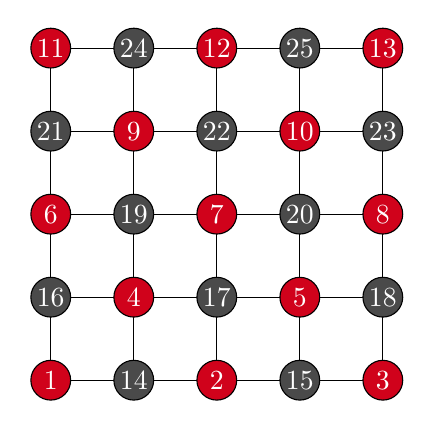
\begin{tikzpicture}[x=0.75pt,y=0.75pt,yscale=-2,xscale=2]
%uncomment if require: \path (0,222); %set diagram left start at 0, and has height of 222

%Shape: Grid [id:dp7509010194001084] 
\draw  [draw opacity=0][fill={rgb, 255:red, 255; green, 255; blue, 255 }  ,fill opacity=1 ] (289.5,76) -- (369.67,76) -- (369.67,156.5) -- (289.5,156.5) -- cycle ; \draw   (289.5,76) -- (289.5,156.5)(309.5,76) -- (309.5,156.5)(329.5,76) -- (329.5,156.5)(349.5,76) -- (349.5,156.5)(369.5,76) -- (369.5,156.5) ; \draw   (289.5,76) -- (369.67,76)(289.5,96) -- (369.67,96)(289.5,116) -- (369.67,116)(289.5,136) -- (369.67,136)(289.5,156) -- (369.67,156) ; \draw    ;
%Shape: Circle [id:dp6108755291859196] 
\draw  [fill={rgb, 255:red, 208; green, 2; blue, 27 }  ,fill opacity=1 ] (284.71,156) .. controls (284.71,153.35) and (286.85,151.21) .. (289.5,151.21) .. controls (292.15,151.21) and (294.29,153.35) .. (294.29,156) .. controls (294.29,158.65) and (292.15,160.79) .. (289.5,160.79) .. controls (286.85,160.79) and (284.71,158.65) .. (284.71,156) -- cycle ;
%Shape: Circle [id:dp4441687082516983] 
\draw  [fill={rgb, 255:red, 74; green, 74; blue, 74 }  ,fill opacity=1 ] (304.71,156) .. controls (304.71,153.35) and (306.85,151.21) .. (309.5,151.21) .. controls (312.15,151.21) and (314.29,153.35) .. (314.29,156) .. controls (314.29,158.65) and (312.15,160.79) .. (309.5,160.79) .. controls (306.85,160.79) and (304.71,158.65) .. (304.71,156) -- cycle ;
%Shape: Circle [id:dp6167896316379069] 
\draw  [fill={rgb, 255:red, 208; green, 2; blue, 27 }  ,fill opacity=1 ] (324.71,156) .. controls (324.71,153.35) and (326.85,151.21) .. (329.5,151.21) .. controls (332.15,151.21) and (334.29,153.35) .. (334.29,156) .. controls (334.29,158.65) and (332.15,160.79) .. (329.5,160.79) .. controls (326.85,160.79) and (324.71,158.65) .. (324.71,156) -- cycle ;
%Shape: Circle [id:dp6715236044117903] 
\draw  [fill={rgb, 255:red, 74; green, 74; blue, 74 }  ,fill opacity=1 ] (344.71,156) .. controls (344.71,153.35) and (346.85,151.21) .. (349.5,151.21) .. controls (352.15,151.21) and (354.29,153.35) .. (354.29,156) .. controls (354.29,158.65) and (352.15,160.79) .. (349.5,160.79) .. controls (346.85,160.79) and (344.71,158.65) .. (344.71,156) -- cycle ;
%Shape: Circle [id:dp06410493254248473] 
\draw  [fill={rgb, 255:red, 208; green, 2; blue, 27 }  ,fill opacity=1 ] (364.71,156) .. controls (364.71,153.35) and (366.85,151.21) .. (369.5,151.21) .. controls (372.15,151.21) and (374.29,153.35) .. (374.29,156) .. controls (374.29,158.65) and (372.15,160.79) .. (369.5,160.79) .. controls (366.85,160.79) and (364.71,158.65) .. (364.71,156) -- cycle ;
%Shape: Circle [id:dp6649764858783351] 
\draw  [fill={rgb, 255:red, 208; green, 2; blue, 27 }  ,fill opacity=1 ] (364.71,116) .. controls (364.71,113.35) and (366.85,111.21) .. (369.5,111.21) .. controls (372.15,111.21) and (374.29,113.35) .. (374.29,116) .. controls (374.29,118.65) and (372.15,120.79) .. (369.5,120.79) .. controls (366.85,120.79) and (364.71,118.65) .. (364.71,116) -- cycle ;
%Shape: Circle [id:dp9554900297815432] 
\draw  [fill={rgb, 255:red, 74; green, 74; blue, 74 }  ,fill opacity=1 ] (364.71,136) .. controls (364.71,133.35) and (366.85,131.21) .. (369.5,131.21) .. controls (372.15,131.21) and (374.29,133.35) .. (374.29,136) .. controls (374.29,138.65) and (372.15,140.79) .. (369.5,140.79) .. controls (366.85,140.79) and (364.71,138.65) .. (364.71,136) -- cycle ;
%Shape: Circle [id:dp37112581806137124] 
\draw  [fill={rgb, 255:red, 208; green, 2; blue, 27 }  ,fill opacity=1 ] (344.71,136) .. controls (344.71,133.35) and (346.85,131.21) .. (349.5,131.21) .. controls (352.15,131.21) and (354.29,133.35) .. (354.29,136) .. controls (354.29,138.65) and (352.15,140.79) .. (349.5,140.79) .. controls (346.85,140.79) and (344.71,138.65) .. (344.71,136) -- cycle ;
%Shape: Circle [id:dp06306680838602707] 
\draw  [fill={rgb, 255:red, 74; green, 74; blue, 74 }  ,fill opacity=1 ] (324.71,136) .. controls (324.71,133.35) and (326.85,131.21) .. (329.5,131.21) .. controls (332.15,131.21) and (334.29,133.35) .. (334.29,136) .. controls (334.29,138.65) and (332.15,140.79) .. (329.5,140.79) .. controls (326.85,140.79) and (324.71,138.65) .. (324.71,136) -- cycle ;
%Shape: Circle [id:dp9358022961380756] 
\draw  [fill={rgb, 255:red, 208; green, 2; blue, 27 }  ,fill opacity=1 ] (304.71,136) .. controls (304.71,133.35) and (306.85,131.21) .. (309.5,131.21) .. controls (312.15,131.21) and (314.29,133.35) .. (314.29,136) .. controls (314.29,138.65) and (312.15,140.79) .. (309.5,140.79) .. controls (306.85,140.79) and (304.71,138.65) .. (304.71,136) -- cycle ;
%Shape: Circle [id:dp9068520178890649] 
\draw  [fill={rgb, 255:red, 74; green, 74; blue, 74 }  ,fill opacity=1 ] (284.71,136) .. controls (284.71,133.35) and (286.85,131.21) .. (289.5,131.21) .. controls (292.15,131.21) and (294.29,133.35) .. (294.29,136) .. controls (294.29,138.65) and (292.15,140.79) .. (289.5,140.79) .. controls (286.85,140.79) and (284.71,138.65) .. (284.71,136) -- cycle ;
%Shape: Circle [id:dp8562155796812134] 
\draw  [fill={rgb, 255:red, 208; green, 2; blue, 27 }  ,fill opacity=1 ] (284.71,116) .. controls (284.71,113.35) and (286.85,111.21) .. (289.5,111.21) .. controls (292.15,111.21) and (294.29,113.35) .. (294.29,116) .. controls (294.29,118.65) and (292.15,120.79) .. (289.5,120.79) .. controls (286.85,120.79) and (284.71,118.65) .. (284.71,116) -- cycle ;
%Shape: Circle [id:dp2479839382803859] 
\draw  [fill={rgb, 255:red, 74; green, 74; blue, 74 }  ,fill opacity=1 ] (304.71,116) .. controls (304.71,113.35) and (306.85,111.21) .. (309.5,111.21) .. controls (312.15,111.21) and (314.29,113.35) .. (314.29,116) .. controls (314.29,118.65) and (312.15,120.79) .. (309.5,120.79) .. controls (306.85,120.79) and (304.71,118.65) .. (304.71,116) -- cycle ;
%Shape: Circle [id:dp8339992993489453] 
\draw  [fill={rgb, 255:red, 208; green, 2; blue, 27 }  ,fill opacity=1 ] (324.71,116) .. controls (324.71,113.35) and (326.85,111.21) .. (329.5,111.21) .. controls (332.15,111.21) and (334.29,113.35) .. (334.29,116) .. controls (334.29,118.65) and (332.15,120.79) .. (329.5,120.79) .. controls (326.85,120.79) and (324.71,118.65) .. (324.71,116) -- cycle ;
%Shape: Circle [id:dp29657132974437017] 
\draw  [fill={rgb, 255:red, 74; green, 74; blue, 74 }  ,fill opacity=1 ] (344.71,116) .. controls (344.71,113.35) and (346.85,111.21) .. (349.5,111.21) .. controls (352.15,111.21) and (354.29,113.35) .. (354.29,116) .. controls (354.29,118.65) and (352.15,120.79) .. (349.5,120.79) .. controls (346.85,120.79) and (344.71,118.65) .. (344.71,116) -- cycle ;
%Shape: Circle [id:dp4006844726389853] 
\draw  [fill={rgb, 255:red, 74; green, 74; blue, 74 }  ,fill opacity=1 ] (284.71,96) .. controls (284.71,93.35) and (286.85,91.21) .. (289.5,91.21) .. controls (292.15,91.21) and (294.29,93.35) .. (294.29,96) .. controls (294.29,98.65) and (292.15,100.79) .. (289.5,100.79) .. controls (286.85,100.79) and (284.71,98.65) .. (284.71,96) -- cycle ;
%Shape: Circle [id:dp2518725902881924] 
\draw  [fill={rgb, 255:red, 208; green, 2; blue, 27 }  ,fill opacity=1 ] (304.71,96) .. controls (304.71,93.35) and (306.85,91.21) .. (309.5,91.21) .. controls (312.15,91.21) and (314.29,93.35) .. (314.29,96) .. controls (314.29,98.65) and (312.15,100.79) .. (309.5,100.79) .. controls (306.85,100.79) and (304.71,98.65) .. (304.71,96) -- cycle ;
%Shape: Circle [id:dp9478829895408571] 
\draw  [fill={rgb, 255:red, 74; green, 74; blue, 74 }  ,fill opacity=1 ] (324.71,96) .. controls (324.71,93.35) and (326.85,91.21) .. (329.5,91.21) .. controls (332.15,91.21) and (334.29,93.35) .. (334.29,96) .. controls (334.29,98.65) and (332.15,100.79) .. (329.5,100.79) .. controls (326.85,100.79) and (324.71,98.65) .. (324.71,96) -- cycle ;
%Shape: Circle [id:dp5111042484735311] 
\draw  [fill={rgb, 255:red, 208; green, 2; blue, 27 }  ,fill opacity=1 ] (344.71,96) .. controls (344.71,93.35) and (346.85,91.21) .. (349.5,91.21) .. controls (352.15,91.21) and (354.29,93.35) .. (354.29,96) .. controls (354.29,98.65) and (352.15,100.79) .. (349.5,100.79) .. controls (346.85,100.79) and (344.71,98.65) .. (344.71,96) -- cycle ;
%Shape: Circle [id:dp08226041749176072] 
\draw  [fill={rgb, 255:red, 74; green, 74; blue, 74 }  ,fill opacity=1 ] (364.71,96) .. controls (364.71,93.35) and (366.85,91.21) .. (369.5,91.21) .. controls (372.15,91.21) and (374.29,93.35) .. (374.29,96) .. controls (374.29,98.65) and (372.15,100.79) .. (369.5,100.79) .. controls (366.85,100.79) and (364.71,98.65) .. (364.71,96) -- cycle ;
%Shape: Circle [id:dp6793036732090996] 
\draw  [fill={rgb, 255:red, 208; green, 2; blue, 27 }  ,fill opacity=1 ] (284.71,76) .. controls (284.71,73.35) and (286.85,71.21) .. (289.5,71.21) .. controls (292.15,71.21) and (294.29,73.35) .. (294.29,76) .. controls (294.29,78.65) and (292.15,80.79) .. (289.5,80.79) .. controls (286.85,80.79) and (284.71,78.65) .. (284.71,76) -- cycle ;
%Shape: Circle [id:dp4959600894339744] 
\draw  [fill={rgb, 255:red, 74; green, 74; blue, 74 }  ,fill opacity=1 ] (304.71,76) .. controls (304.71,73.35) and (306.85,71.21) .. (309.5,71.21) .. controls (312.15,71.21) and (314.29,73.35) .. (314.29,76) .. controls (314.29,78.65) and (312.15,80.79) .. (309.5,80.79) .. controls (306.85,80.79) and (304.71,78.65) .. (304.71,76) -- cycle ;
%Shape: Circle [id:dp9621563131775881] 
\draw  [fill={rgb, 255:red, 208; green, 2; blue, 27 }  ,fill opacity=1 ] (324.71,76) .. controls (324.71,73.35) and (326.85,71.21) .. (329.5,71.21) .. controls (332.15,71.21) and (334.29,73.35) .. (334.29,76) .. controls (334.29,78.65) and (332.15,80.79) .. (329.5,80.79) .. controls (326.85,80.79) and (324.71,78.65) .. (324.71,76) -- cycle ;
%Shape: Circle [id:dp06302816821338242] 
\draw  [fill={rgb, 255:red, 74; green, 74; blue, 74 }  ,fill opacity=1 ] (344.71,76) .. controls (344.71,73.35) and (346.85,71.21) .. (349.5,71.21) .. controls (352.15,71.21) and (354.29,73.35) .. (354.29,76) .. controls (354.29,78.65) and (352.15,80.79) .. (349.5,80.79) .. controls (346.85,80.79) and (344.71,78.65) .. (344.71,76) -- cycle ;
%Shape: Circle [id:dp40969700298757994] 
\draw  [fill={rgb, 255:red, 208; green, 2; blue, 27 }  ,fill opacity=1 ] (364.71,76) .. controls (364.71,73.35) and (366.85,71.21) .. (369.5,71.21) .. controls (372.15,71.21) and (374.29,73.35) .. (374.29,76) .. controls (374.29,78.65) and (372.15,80.79) .. (369.5,80.79) .. controls (366.85,80.79) and (364.71,78.65) .. (364.71,76) -- cycle ;

% Text Node
\draw (289.5,156) node [scale=1,color={rgb, 255:red, 255; green, 255; blue, 255 }  ,opacity=1 ] [align=left] {1};
% Text Node
\draw (329.5,156) node [scale=1,color={rgb, 255:red, 255; green, 255; blue, 255 }  ,opacity=1 ] [align=left] {2};
% Text Node
\draw (369.5,156) node [scale=1,color={rgb, 255:red, 255; green, 255; blue, 255 }  ,opacity=1 ] [align=left] {3};
% Text Node
\draw (309.5,136) node [scale=1,color={rgb, 255:red, 255; green, 255; blue, 255 }  ,opacity=1 ] [align=left] {4};
% Text Node
\draw (349.5,136) node [scale=1,color={rgb, 255:red, 255; green, 255; blue, 255 }  ,opacity=1 ] [align=left] {5};
% Text Node
\draw (289.5,116) node [scale=1,color={rgb, 255:red, 255; green, 255; blue, 255 }  ,opacity=1 ] [align=left] {6};
% Text Node
\draw (329.5,116) node [scale=1,color={rgb, 255:red, 255; green, 255; blue, 255 }  ,opacity=1 ] [align=left] {7};
% Text Node
\draw (369.5,116) node [scale=1,color={rgb, 255:red, 255; green, 255; blue, 255 }  ,opacity=1 ] [align=left] {8};
% Text Node
\draw (309.5,96) node [scale=1,color={rgb, 255:red, 255; green, 255; blue, 255 }  ,opacity=1 ] [align=left] {9};
% Text Node
\draw (349.5,96) node [scale=1,color={rgb, 255:red, 255; green, 255; blue, 255 }  ,opacity=1 ] [align=left] {10};
% Text Node
\draw (289.5,76) node [scale=1,color={rgb, 255:red, 255; green, 255; blue, 255 }  ,opacity=1 ] [align=left] {11};
% Text Node
\draw (329.5,76) node [scale=1,color={rgb, 255:red, 255; green, 255; blue, 255 }  ,opacity=1 ] [align=left] {12};
% Text Node
\draw (369.5,76) node [scale=1,color={rgb, 255:red, 255; green, 255; blue, 255 }  ,opacity=1 ] [align=left] {13};
% Text Node
\draw (309.5,156) node [scale=1,color={rgb, 255:red, 255; green, 255; blue, 255 }  ,opacity=1 ] [align=left] {14};
% Text Node
\draw (349.5,156) node [scale=1,color={rgb, 255:red, 255; green, 255; blue, 255 }  ,opacity=1 ] [align=left] {15};
% Text Node
\draw (289.5,136) node [scale=1,color={rgb, 255:red, 255; green, 255; blue, 255 }  ,opacity=1 ] [align=left] {16};
% Text Node
\draw (329.5,136) node [scale=1,color={rgb, 255:red, 255; green, 255; blue, 255 }  ,opacity=1 ] [align=left] {17};
% Text Node
\draw (369.5,136) node [scale=1,color={rgb, 255:red, 255; green, 255; blue, 255 }  ,opacity=1 ] [align=left] {18};
% Text Node
\draw (309.5,116) node [scale=1,color={rgb, 255:red, 255; green, 255; blue, 255 }  ,opacity=1 ] [align=left] {19};
% Text Node
\draw (349.5,116) node [scale=1,color={rgb, 255:red, 255; green, 255; blue, 255 }  ,opacity=1 ] [align=left] {20};
% Text Node
\draw (289.5,96) node [scale=1,color={rgb, 255:red, 255; green, 255; blue, 255 }  ,opacity=1 ] [align=left] {21};
% Text Node
\draw (329.5,96) node [scale=1,color={rgb, 255:red, 255; green, 255; blue, 255 }  ,opacity=1 ] [align=left] {22};
% Text Node
\draw (369.5,96) node [scale=1,color={rgb, 255:red, 255; green, 255; blue, 255 }  ,opacity=1 ] [align=left] {23};
% Text Node
\draw (309.5,76) node [scale=1,color={rgb, 255:red, 255; green, 255; blue, 255 }  ,opacity=1 ] [align=left] {24};
% Text Node
\draw (349.5,76) node [scale=1,color={rgb, 255:red, 255; green, 255; blue, 255 }  ,opacity=1 ] [align=left] {25};


\end{tikzpicture}

			\end{center}
			\caption{Red-Black ordering}
			\label{fig:redblackorder}
		\end{figure}

		Question 1: How many colors do you need in 3D?

		Question 2: Does an analytic expression for $l(i,j)$ exist?
	\item Cache-aware ordering (Cluster nodes into connected groups)

		\begin{figure}[ht!]
			\begin{center}
				

\tikzset{every picture/.style={line width=0.75pt}} %set default line width to 0.75pt        

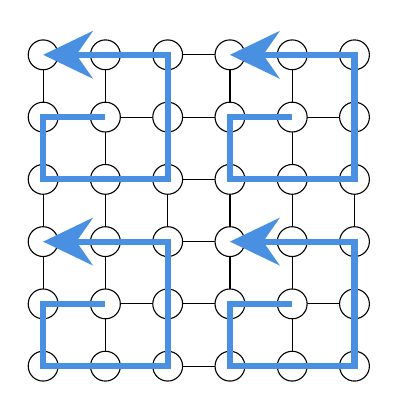
\begin{tikzpicture}[x=0.75pt,y=0.75pt,yscale=-1.5,xscale=1.5]
%uncomment if require: \path (0,301); %set diagram left start at 0, and has height of 301

%Shape: Grid [id:dp04007873776394999] 
\draw  [draw opacity=0][fill={rgb, 255:red, 255; green, 255; blue, 255 }  ,fill opacity=1 ] (280.5,104) -- (380.83,104) -- (380.83,204.33) -- (280.5,204.33) -- cycle ; \draw   (280.5,104) -- (280.5,204.33)(300.5,104) -- (300.5,204.33)(320.5,104) -- (320.5,204.33)(340.5,104) -- (340.5,204.33)(360.5,104) -- (360.5,204.33)(380.5,104) -- (380.5,204.33) ; \draw   (280.5,104) -- (380.83,104)(280.5,124) -- (380.83,124)(280.5,144) -- (380.83,144)(280.5,164) -- (380.83,164)(280.5,184) -- (380.83,184)(280.5,204) -- (380.83,204) ; \draw    ;
%Shape: Circle [id:dp9474225282412638] 
\draw  [fill={rgb, 255:red, 255; green, 255; blue, 255 }  ,fill opacity=1 ] (275.71,184) .. controls (275.71,181.35) and (277.85,179.21) .. (280.5,179.21) .. controls (283.15,179.21) and (285.29,181.35) .. (285.29,184) .. controls (285.29,186.65) and (283.15,188.79) .. (280.5,188.79) .. controls (277.85,188.79) and (275.71,186.65) .. (275.71,184) -- cycle ;
%Shape: Circle [id:dp16610143440847636] 
\draw  [fill={rgb, 255:red, 255; green, 255; blue, 255 }  ,fill opacity=1 ] (295.71,184) .. controls (295.71,181.35) and (297.85,179.21) .. (300.5,179.21) .. controls (303.15,179.21) and (305.29,181.35) .. (305.29,184) .. controls (305.29,186.65) and (303.15,188.79) .. (300.5,188.79) .. controls (297.85,188.79) and (295.71,186.65) .. (295.71,184) -- cycle ;
%Shape: Circle [id:dp03456232735817655] 
\draw  [fill={rgb, 255:red, 255; green, 255; blue, 255 }  ,fill opacity=1 ] (315.71,184) .. controls (315.71,181.35) and (317.85,179.21) .. (320.5,179.21) .. controls (323.15,179.21) and (325.29,181.35) .. (325.29,184) .. controls (325.29,186.65) and (323.15,188.79) .. (320.5,188.79) .. controls (317.85,188.79) and (315.71,186.65) .. (315.71,184) -- cycle ;
%Shape: Circle [id:dp5584249108368513] 
\draw  [fill={rgb, 255:red, 255; green, 255; blue, 255 }  ,fill opacity=1 ] (335.71,184) .. controls (335.71,181.35) and (337.85,179.21) .. (340.5,179.21) .. controls (343.15,179.21) and (345.29,181.35) .. (345.29,184) .. controls (345.29,186.65) and (343.15,188.79) .. (340.5,188.79) .. controls (337.85,188.79) and (335.71,186.65) .. (335.71,184) -- cycle ;
%Shape: Circle [id:dp16243430214118293] 
\draw  [fill={rgb, 255:red, 255; green, 255; blue, 255 }  ,fill opacity=1 ] (355.71,184) .. controls (355.71,181.35) and (357.85,179.21) .. (360.5,179.21) .. controls (363.15,179.21) and (365.29,181.35) .. (365.29,184) .. controls (365.29,186.65) and (363.15,188.79) .. (360.5,188.79) .. controls (357.85,188.79) and (355.71,186.65) .. (355.71,184) -- cycle ;
%Shape: Circle [id:dp16506904974813086] 
\draw  [fill={rgb, 255:red, 255; green, 255; blue, 255 }  ,fill opacity=1 ] (355.71,144) .. controls (355.71,141.35) and (357.85,139.21) .. (360.5,139.21) .. controls (363.15,139.21) and (365.29,141.35) .. (365.29,144) .. controls (365.29,146.65) and (363.15,148.79) .. (360.5,148.79) .. controls (357.85,148.79) and (355.71,146.65) .. (355.71,144) -- cycle ;
%Shape: Circle [id:dp021230581558282724] 
\draw  [fill={rgb, 255:red, 255; green, 255; blue, 255 }  ,fill opacity=1 ] (355.71,164) .. controls (355.71,161.35) and (357.85,159.21) .. (360.5,159.21) .. controls (363.15,159.21) and (365.29,161.35) .. (365.29,164) .. controls (365.29,166.65) and (363.15,168.79) .. (360.5,168.79) .. controls (357.85,168.79) and (355.71,166.65) .. (355.71,164) -- cycle ;
%Shape: Circle [id:dp1804479365808369] 
\draw  [fill={rgb, 255:red, 255; green, 255; blue, 255 }  ,fill opacity=1 ] (335.71,164) .. controls (335.71,161.35) and (337.85,159.21) .. (340.5,159.21) .. controls (343.15,159.21) and (345.29,161.35) .. (345.29,164) .. controls (345.29,166.65) and (343.15,168.79) .. (340.5,168.79) .. controls (337.85,168.79) and (335.71,166.65) .. (335.71,164) -- cycle ;
%Shape: Circle [id:dp47675744505678375] 
\draw  [fill={rgb, 255:red, 255; green, 255; blue, 255 }  ,fill opacity=1 ] (315.71,164) .. controls (315.71,161.35) and (317.85,159.21) .. (320.5,159.21) .. controls (323.15,159.21) and (325.29,161.35) .. (325.29,164) .. controls (325.29,166.65) and (323.15,168.79) .. (320.5,168.79) .. controls (317.85,168.79) and (315.71,166.65) .. (315.71,164) -- cycle ;
%Shape: Circle [id:dp7334743663555192] 
\draw  [fill={rgb, 255:red, 255; green, 255; blue, 255 }  ,fill opacity=1 ] (295.71,164) .. controls (295.71,161.35) and (297.85,159.21) .. (300.5,159.21) .. controls (303.15,159.21) and (305.29,161.35) .. (305.29,164) .. controls (305.29,166.65) and (303.15,168.79) .. (300.5,168.79) .. controls (297.85,168.79) and (295.71,166.65) .. (295.71,164) -- cycle ;
%Shape: Circle [id:dp3042824921088443] 
\draw  [fill={rgb, 255:red, 255; green, 255; blue, 255 }  ,fill opacity=1 ] (275.71,164) .. controls (275.71,161.35) and (277.85,159.21) .. (280.5,159.21) .. controls (283.15,159.21) and (285.29,161.35) .. (285.29,164) .. controls (285.29,166.65) and (283.15,168.79) .. (280.5,168.79) .. controls (277.85,168.79) and (275.71,166.65) .. (275.71,164) -- cycle ;
%Shape: Circle [id:dp15842066644056607] 
\draw  [fill={rgb, 255:red, 255; green, 255; blue, 255 }  ,fill opacity=1 ] (275.71,144) .. controls (275.71,141.35) and (277.85,139.21) .. (280.5,139.21) .. controls (283.15,139.21) and (285.29,141.35) .. (285.29,144) .. controls (285.29,146.65) and (283.15,148.79) .. (280.5,148.79) .. controls (277.85,148.79) and (275.71,146.65) .. (275.71,144) -- cycle ;
%Shape: Circle [id:dp29704787273716904] 
\draw  [fill={rgb, 255:red, 255; green, 255; blue, 255 }  ,fill opacity=1 ] (295.71,144) .. controls (295.71,141.35) and (297.85,139.21) .. (300.5,139.21) .. controls (303.15,139.21) and (305.29,141.35) .. (305.29,144) .. controls (305.29,146.65) and (303.15,148.79) .. (300.5,148.79) .. controls (297.85,148.79) and (295.71,146.65) .. (295.71,144) -- cycle ;
%Shape: Circle [id:dp15622750086846238] 
\draw  [fill={rgb, 255:red, 255; green, 255; blue, 255 }  ,fill opacity=1 ] (315.71,144) .. controls (315.71,141.35) and (317.85,139.21) .. (320.5,139.21) .. controls (323.15,139.21) and (325.29,141.35) .. (325.29,144) .. controls (325.29,146.65) and (323.15,148.79) .. (320.5,148.79) .. controls (317.85,148.79) and (315.71,146.65) .. (315.71,144) -- cycle ;
%Shape: Circle [id:dp8093803696218231] 
\draw  [fill={rgb, 255:red, 255; green, 255; blue, 255 }  ,fill opacity=1 ] (335.71,144) .. controls (335.71,141.35) and (337.85,139.21) .. (340.5,139.21) .. controls (343.15,139.21) and (345.29,141.35) .. (345.29,144) .. controls (345.29,146.65) and (343.15,148.79) .. (340.5,148.79) .. controls (337.85,148.79) and (335.71,146.65) .. (335.71,144) -- cycle ;
%Shape: Circle [id:dp10695862196164163] 
\draw  [fill={rgb, 255:red, 255; green, 255; blue, 255 }  ,fill opacity=1 ] (275.71,124) .. controls (275.71,121.35) and (277.85,119.21) .. (280.5,119.21) .. controls (283.15,119.21) and (285.29,121.35) .. (285.29,124) .. controls (285.29,126.65) and (283.15,128.79) .. (280.5,128.79) .. controls (277.85,128.79) and (275.71,126.65) .. (275.71,124) -- cycle ;
%Shape: Circle [id:dp5260605006362917] 
\draw  [fill={rgb, 255:red, 255; green, 255; blue, 255 }  ,fill opacity=1 ] (295.71,124) .. controls (295.71,121.35) and (297.85,119.21) .. (300.5,119.21) .. controls (303.15,119.21) and (305.29,121.35) .. (305.29,124) .. controls (305.29,126.65) and (303.15,128.79) .. (300.5,128.79) .. controls (297.85,128.79) and (295.71,126.65) .. (295.71,124) -- cycle ;
%Shape: Circle [id:dp8473153436273366] 
\draw  [fill={rgb, 255:red, 255; green, 255; blue, 255 }  ,fill opacity=1 ] (315.71,124) .. controls (315.71,121.35) and (317.85,119.21) .. (320.5,119.21) .. controls (323.15,119.21) and (325.29,121.35) .. (325.29,124) .. controls (325.29,126.65) and (323.15,128.79) .. (320.5,128.79) .. controls (317.85,128.79) and (315.71,126.65) .. (315.71,124) -- cycle ;
%Shape: Circle [id:dp7857758511872395] 
\draw  [fill={rgb, 255:red, 255; green, 255; blue, 255 }  ,fill opacity=1 ] (335.71,124) .. controls (335.71,121.35) and (337.85,119.21) .. (340.5,119.21) .. controls (343.15,119.21) and (345.29,121.35) .. (345.29,124) .. controls (345.29,126.65) and (343.15,128.79) .. (340.5,128.79) .. controls (337.85,128.79) and (335.71,126.65) .. (335.71,124) -- cycle ;
%Shape: Circle [id:dp3662097810280891] 
\draw  [fill={rgb, 255:red, 255; green, 255; blue, 255 }  ,fill opacity=1 ] (355.71,124) .. controls (355.71,121.35) and (357.85,119.21) .. (360.5,119.21) .. controls (363.15,119.21) and (365.29,121.35) .. (365.29,124) .. controls (365.29,126.65) and (363.15,128.79) .. (360.5,128.79) .. controls (357.85,128.79) and (355.71,126.65) .. (355.71,124) -- cycle ;
%Shape: Circle [id:dp05943436716946482] 
\draw  [fill={rgb, 255:red, 255; green, 255; blue, 255 }  ,fill opacity=1 ] (275.71,104) .. controls (275.71,101.35) and (277.85,99.21) .. (280.5,99.21) .. controls (283.15,99.21) and (285.29,101.35) .. (285.29,104) .. controls (285.29,106.65) and (283.15,108.79) .. (280.5,108.79) .. controls (277.85,108.79) and (275.71,106.65) .. (275.71,104) -- cycle ;
%Shape: Circle [id:dp809722377804333] 
\draw  [fill={rgb, 255:red, 255; green, 255; blue, 255 }  ,fill opacity=1 ] (295.71,104) .. controls (295.71,101.35) and (297.85,99.21) .. (300.5,99.21) .. controls (303.15,99.21) and (305.29,101.35) .. (305.29,104) .. controls (305.29,106.65) and (303.15,108.79) .. (300.5,108.79) .. controls (297.85,108.79) and (295.71,106.65) .. (295.71,104) -- cycle ;
%Shape: Circle [id:dp2456656687962917] 
\draw  [fill={rgb, 255:red, 255; green, 255; blue, 255 }  ,fill opacity=1 ] (315.71,104) .. controls (315.71,101.35) and (317.85,99.21) .. (320.5,99.21) .. controls (323.15,99.21) and (325.29,101.35) .. (325.29,104) .. controls (325.29,106.65) and (323.15,108.79) .. (320.5,108.79) .. controls (317.85,108.79) and (315.71,106.65) .. (315.71,104) -- cycle ;
%Shape: Circle [id:dp4412509805400553] 
\draw  [fill={rgb, 255:red, 255; green, 255; blue, 255 }  ,fill opacity=1 ] (335.71,104) .. controls (335.71,101.35) and (337.85,99.21) .. (340.5,99.21) .. controls (343.15,99.21) and (345.29,101.35) .. (345.29,104) .. controls (345.29,106.65) and (343.15,108.79) .. (340.5,108.79) .. controls (337.85,108.79) and (335.71,106.65) .. (335.71,104) -- cycle ;
%Shape: Circle [id:dp9250884814038944] 
\draw  [fill={rgb, 255:red, 255; green, 255; blue, 255 }  ,fill opacity=1 ] (355.71,104) .. controls (355.71,101.35) and (357.85,99.21) .. (360.5,99.21) .. controls (363.15,99.21) and (365.29,101.35) .. (365.29,104) .. controls (365.29,106.65) and (363.15,108.79) .. (360.5,108.79) .. controls (357.85,108.79) and (355.71,106.65) .. (355.71,104) -- cycle ;
%Shape: Circle [id:dp5750759061407391] 
\draw  [fill={rgb, 255:red, 255; green, 255; blue, 255 }  ,fill opacity=1 ] (375.71,104) .. controls (375.71,101.35) and (377.85,99.21) .. (380.5,99.21) .. controls (383.15,99.21) and (385.29,101.35) .. (385.29,104) .. controls (385.29,106.65) and (383.15,108.79) .. (380.5,108.79) .. controls (377.85,108.79) and (375.71,106.65) .. (375.71,104) -- cycle ;
%Shape: Circle [id:dp31417490416250016] 
\draw  [fill={rgb, 255:red, 255; green, 255; blue, 255 }  ,fill opacity=1 ] (375.71,124) .. controls (375.71,121.35) and (377.85,119.21) .. (380.5,119.21) .. controls (383.15,119.21) and (385.29,121.35) .. (385.29,124) .. controls (385.29,126.65) and (383.15,128.79) .. (380.5,128.79) .. controls (377.85,128.79) and (375.71,126.65) .. (375.71,124) -- cycle ;
%Shape: Circle [id:dp006667999859743423] 
\draw  [fill={rgb, 255:red, 255; green, 255; blue, 255 }  ,fill opacity=1 ] (375.71,144) .. controls (375.71,141.35) and (377.85,139.21) .. (380.5,139.21) .. controls (383.15,139.21) and (385.29,141.35) .. (385.29,144) .. controls (385.29,146.65) and (383.15,148.79) .. (380.5,148.79) .. controls (377.85,148.79) and (375.71,146.65) .. (375.71,144) -- cycle ;
%Shape: Circle [id:dp12634282620893122] 
\draw  [fill={rgb, 255:red, 255; green, 255; blue, 255 }  ,fill opacity=1 ] (375.71,164) .. controls (375.71,161.35) and (377.85,159.21) .. (380.5,159.21) .. controls (383.15,159.21) and (385.29,161.35) .. (385.29,164) .. controls (385.29,166.65) and (383.15,168.79) .. (380.5,168.79) .. controls (377.85,168.79) and (375.71,166.65) .. (375.71,164) -- cycle ;
%Shape: Circle [id:dp19045978877802572] 
\draw  [fill={rgb, 255:red, 255; green, 255; blue, 255 }  ,fill opacity=1 ] (275.71,204) .. controls (275.71,201.35) and (277.85,199.21) .. (280.5,199.21) .. controls (283.15,199.21) and (285.29,201.35) .. (285.29,204) .. controls (285.29,206.65) and (283.15,208.79) .. (280.5,208.79) .. controls (277.85,208.79) and (275.71,206.65) .. (275.71,204) -- cycle ;
%Shape: Circle [id:dp8417560897443137] 
\draw  [fill={rgb, 255:red, 255; green, 255; blue, 255 }  ,fill opacity=1 ] (295.71,204) .. controls (295.71,201.35) and (297.85,199.21) .. (300.5,199.21) .. controls (303.15,199.21) and (305.29,201.35) .. (305.29,204) .. controls (305.29,206.65) and (303.15,208.79) .. (300.5,208.79) .. controls (297.85,208.79) and (295.71,206.65) .. (295.71,204) -- cycle ;
%Shape: Circle [id:dp36466854494079004] 
\draw  [fill={rgb, 255:red, 255; green, 255; blue, 255 }  ,fill opacity=1 ] (315.71,204) .. controls (315.71,201.35) and (317.85,199.21) .. (320.5,199.21) .. controls (323.15,199.21) and (325.29,201.35) .. (325.29,204) .. controls (325.29,206.65) and (323.15,208.79) .. (320.5,208.79) .. controls (317.85,208.79) and (315.71,206.65) .. (315.71,204) -- cycle ;
%Shape: Circle [id:dp08813117271342974] 
\draw  [fill={rgb, 255:red, 255; green, 255; blue, 255 }  ,fill opacity=1 ] (335.71,204) .. controls (335.71,201.35) and (337.85,199.21) .. (340.5,199.21) .. controls (343.15,199.21) and (345.29,201.35) .. (345.29,204) .. controls (345.29,206.65) and (343.15,208.79) .. (340.5,208.79) .. controls (337.85,208.79) and (335.71,206.65) .. (335.71,204) -- cycle ;
%Shape: Circle [id:dp12510148076826888] 
\draw  [fill={rgb, 255:red, 255; green, 255; blue, 255 }  ,fill opacity=1 ] (355.71,204) .. controls (355.71,201.35) and (357.85,199.21) .. (360.5,199.21) .. controls (363.15,199.21) and (365.29,201.35) .. (365.29,204) .. controls (365.29,206.65) and (363.15,208.79) .. (360.5,208.79) .. controls (357.85,208.79) and (355.71,206.65) .. (355.71,204) -- cycle ;
%Shape: Circle [id:dp32302714489826934] 
\draw  [fill={rgb, 255:red, 255; green, 255; blue, 255 }  ,fill opacity=1 ] (375.71,204) .. controls (375.71,201.35) and (377.85,199.21) .. (380.5,199.21) .. controls (383.15,199.21) and (385.29,201.35) .. (385.29,204) .. controls (385.29,206.65) and (383.15,208.79) .. (380.5,208.79) .. controls (377.85,208.79) and (375.71,206.65) .. (375.71,204) -- cycle ;
%Shape: Circle [id:dp047477242771539085] 
\draw  [fill={rgb, 255:red, 255; green, 255; blue, 255 }  ,fill opacity=1 ] (375.71,184) .. controls (375.71,181.35) and (377.85,179.21) .. (380.5,179.21) .. controls (383.15,179.21) and (385.29,181.35) .. (385.29,184) .. controls (385.29,186.65) and (383.15,188.79) .. (380.5,188.79) .. controls (377.85,188.79) and (375.71,186.65) .. (375.71,184) -- cycle ;
%Straight Lines [id:da9724777887310767] 
\draw [color={rgb, 255:red, 74; green, 144; blue, 226 }  ,draw opacity=1 ][line width=2.25]    (300.5,124) -- (280.5,124) -- (280.5,144) -- (320.5,144) -- (320.5,104) -- (284.5,104) ;
\draw [shift={(280.5,104)}, rotate = 360] [fill={rgb, 255:red, 74; green, 144; blue, 226 }  ,fill opacity=1 ][line width=2.25]  [draw opacity=0] (16.07,-7.72) -- (0,0) -- (16.07,7.72) -- (10.67,0) -- cycle    ;

%Straight Lines [id:da17976314984393982] 
\draw [color={rgb, 255:red, 74; green, 144; blue, 226 }  ,draw opacity=1 ][line width=2.25]    (360.5,124) -- (340.5,124) -- (340.5,144) -- (380.5,144) -- (380.5,104) -- (344.5,104) ;
\draw [shift={(340.5,104)}, rotate = 360] [fill={rgb, 255:red, 74; green, 144; blue, 226 }  ,fill opacity=1 ][line width=2.25]  [draw opacity=0] (16.07,-7.72) -- (0,0) -- (16.07,7.72) -- (10.67,0) -- cycle    ;

%Straight Lines [id:da7541239074637796] 
\draw [color={rgb, 255:red, 74; green, 144; blue, 226 }  ,draw opacity=1 ][line width=2.25]    (300.5,184) -- (280.5,184) -- (280.5,204) -- (320.5,204) -- (320.5,164) -- (284.5,164) ;
\draw [shift={(280.5,164)}, rotate = 360] [fill={rgb, 255:red, 74; green, 144; blue, 226 }  ,fill opacity=1 ][line width=2.25]  [draw opacity=0] (16.07,-7.72) -- (0,0) -- (16.07,7.72) -- (10.67,0) -- cycle    ;

%Straight Lines [id:da7981579653949769] 
\draw [color={rgb, 255:red, 74; green, 144; blue, 226 }  ,draw opacity=1 ][line width=2.25]    (360.5,184) -- (340.5,184) -- (340.5,204) -- (380.5,204) -- (380.5,164) -- (344.5,164) ;
\draw [shift={(340.5,164)}, rotate = 360] [fill={rgb, 255:red, 74; green, 144; blue, 226 }  ,fill opacity=1 ][line width=2.25]  [draw opacity=0] (16.07,-7.72) -- (0,0) -- (16.07,7.72) -- (10.67,0) -- cycle    ;





\end{tikzpicture}

			\end{center}
			\caption{Cache-aware ordering, enumeration along the arrow lines}
			\label{fig:cacheorder}
		\end{figure}
		
		This ordering scheme utilizes the fact, that data which is "located in a neighbourhood in memory respectively" can be accessed much quicker and thus fastens the operations used on the matrices.

	\item Wave front orderings (diagonal ordering)

		\begin{figure}[ht!]
			\begin{center}
				

\tikzset{every picture/.style={line width=0.75pt}} %set default line width to 0.75pt        

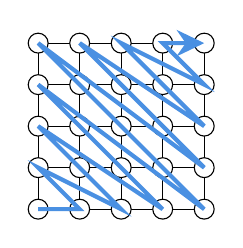
\begin{tikzpicture}[x=0.75pt,y=0.75pt,yscale=-1,xscale=1]
%uncomment if require: \path (0,260); %set diagram left start at 0, and has height of 260

%Shape: Grid [id:dp23256726802759253] 
\draw  [draw opacity=0][fill={rgb, 255:red, 255; green, 255; blue, 255 }  ,fill opacity=1 ] (290.5,90) -- (370.67,90) -- (370.67,170.5) -- (290.5,170.5) -- cycle ; \draw   (290.5,90) -- (290.5,170.5)(310.5,90) -- (310.5,170.5)(330.5,90) -- (330.5,170.5)(350.5,90) -- (350.5,170.5)(370.5,90) -- (370.5,170.5) ; \draw   (290.5,90) -- (370.67,90)(290.5,110) -- (370.67,110)(290.5,130) -- (370.67,130)(290.5,150) -- (370.67,150)(290.5,170) -- (370.67,170) ; \draw    ;
%Shape: Circle [id:dp8205642245940685] 
\draw  [fill={rgb, 255:red, 255; green, 255; blue, 255 }  ,fill opacity=1 ] (285.71,170) .. controls (285.71,167.35) and (287.85,165.21) .. (290.5,165.21) .. controls (293.15,165.21) and (295.29,167.35) .. (295.29,170) .. controls (295.29,172.65) and (293.15,174.79) .. (290.5,174.79) .. controls (287.85,174.79) and (285.71,172.65) .. (285.71,170) -- cycle ;
%Shape: Circle [id:dp366405571034746] 
\draw  [fill={rgb, 255:red, 255; green, 255; blue, 255 }  ,fill opacity=1 ] (305.71,170) .. controls (305.71,167.35) and (307.85,165.21) .. (310.5,165.21) .. controls (313.15,165.21) and (315.29,167.35) .. (315.29,170) .. controls (315.29,172.65) and (313.15,174.79) .. (310.5,174.79) .. controls (307.85,174.79) and (305.71,172.65) .. (305.71,170) -- cycle ;
%Shape: Circle [id:dp15906627820442676] 
\draw  [fill={rgb, 255:red, 255; green, 255; blue, 255 }  ,fill opacity=1 ] (325.71,170) .. controls (325.71,167.35) and (327.85,165.21) .. (330.5,165.21) .. controls (333.15,165.21) and (335.29,167.35) .. (335.29,170) .. controls (335.29,172.65) and (333.15,174.79) .. (330.5,174.79) .. controls (327.85,174.79) and (325.71,172.65) .. (325.71,170) -- cycle ;
%Shape: Circle [id:dp40387678987476283] 
\draw  [fill={rgb, 255:red, 255; green, 255; blue, 255 }  ,fill opacity=1 ] (345.71,170) .. controls (345.71,167.35) and (347.85,165.21) .. (350.5,165.21) .. controls (353.15,165.21) and (355.29,167.35) .. (355.29,170) .. controls (355.29,172.65) and (353.15,174.79) .. (350.5,174.79) .. controls (347.85,174.79) and (345.71,172.65) .. (345.71,170) -- cycle ;
%Shape: Circle [id:dp004033840648062892] 
\draw  [fill={rgb, 255:red, 255; green, 255; blue, 255 }  ,fill opacity=1 ] (365.71,170) .. controls (365.71,167.35) and (367.85,165.21) .. (370.5,165.21) .. controls (373.15,165.21) and (375.29,167.35) .. (375.29,170) .. controls (375.29,172.65) and (373.15,174.79) .. (370.5,174.79) .. controls (367.85,174.79) and (365.71,172.65) .. (365.71,170) -- cycle ;
%Shape: Circle [id:dp7856406790445534] 
\draw  [fill={rgb, 255:red, 255; green, 255; blue, 255 }  ,fill opacity=1 ] (365.71,130) .. controls (365.71,127.35) and (367.85,125.21) .. (370.5,125.21) .. controls (373.15,125.21) and (375.29,127.35) .. (375.29,130) .. controls (375.29,132.65) and (373.15,134.79) .. (370.5,134.79) .. controls (367.85,134.79) and (365.71,132.65) .. (365.71,130) -- cycle ;
%Shape: Circle [id:dp9423249034074639] 
\draw  [fill={rgb, 255:red, 255; green, 255; blue, 255 }  ,fill opacity=1 ] (365.71,150) .. controls (365.71,147.35) and (367.85,145.21) .. (370.5,145.21) .. controls (373.15,145.21) and (375.29,147.35) .. (375.29,150) .. controls (375.29,152.65) and (373.15,154.79) .. (370.5,154.79) .. controls (367.85,154.79) and (365.71,152.65) .. (365.71,150) -- cycle ;
%Shape: Circle [id:dp4603048926021358] 
\draw  [fill={rgb, 255:red, 255; green, 255; blue, 255 }  ,fill opacity=1 ] (345.71,150) .. controls (345.71,147.35) and (347.85,145.21) .. (350.5,145.21) .. controls (353.15,145.21) and (355.29,147.35) .. (355.29,150) .. controls (355.29,152.65) and (353.15,154.79) .. (350.5,154.79) .. controls (347.85,154.79) and (345.71,152.65) .. (345.71,150) -- cycle ;
%Shape: Circle [id:dp3221609399549774] 
\draw  [fill={rgb, 255:red, 255; green, 255; blue, 255 }  ,fill opacity=1 ] (325.71,150) .. controls (325.71,147.35) and (327.85,145.21) .. (330.5,145.21) .. controls (333.15,145.21) and (335.29,147.35) .. (335.29,150) .. controls (335.29,152.65) and (333.15,154.79) .. (330.5,154.79) .. controls (327.85,154.79) and (325.71,152.65) .. (325.71,150) -- cycle ;
%Shape: Circle [id:dp2913063050312137] 
\draw  [fill={rgb, 255:red, 255; green, 255; blue, 255 }  ,fill opacity=1 ] (305.71,150) .. controls (305.71,147.35) and (307.85,145.21) .. (310.5,145.21) .. controls (313.15,145.21) and (315.29,147.35) .. (315.29,150) .. controls (315.29,152.65) and (313.15,154.79) .. (310.5,154.79) .. controls (307.85,154.79) and (305.71,152.65) .. (305.71,150) -- cycle ;
%Shape: Circle [id:dp08553242219473445] 
\draw  [fill={rgb, 255:red, 255; green, 255; blue, 255 }  ,fill opacity=1 ] (285.71,150) .. controls (285.71,147.35) and (287.85,145.21) .. (290.5,145.21) .. controls (293.15,145.21) and (295.29,147.35) .. (295.29,150) .. controls (295.29,152.65) and (293.15,154.79) .. (290.5,154.79) .. controls (287.85,154.79) and (285.71,152.65) .. (285.71,150) -- cycle ;
%Shape: Circle [id:dp9457745167457556] 
\draw  [fill={rgb, 255:red, 255; green, 255; blue, 255 }  ,fill opacity=1 ] (285.71,130) .. controls (285.71,127.35) and (287.85,125.21) .. (290.5,125.21) .. controls (293.15,125.21) and (295.29,127.35) .. (295.29,130) .. controls (295.29,132.65) and (293.15,134.79) .. (290.5,134.79) .. controls (287.85,134.79) and (285.71,132.65) .. (285.71,130) -- cycle ;
%Shape: Circle [id:dp060234058910684674] 
\draw  [fill={rgb, 255:red, 255; green, 255; blue, 255 }  ,fill opacity=1 ] (305.71,130) .. controls (305.71,127.35) and (307.85,125.21) .. (310.5,125.21) .. controls (313.15,125.21) and (315.29,127.35) .. (315.29,130) .. controls (315.29,132.65) and (313.15,134.79) .. (310.5,134.79) .. controls (307.85,134.79) and (305.71,132.65) .. (305.71,130) -- cycle ;
%Shape: Circle [id:dp9752050660650597] 
\draw  [fill={rgb, 255:red, 255; green, 255; blue, 255 }  ,fill opacity=1 ] (325.71,130) .. controls (325.71,127.35) and (327.85,125.21) .. (330.5,125.21) .. controls (333.15,125.21) and (335.29,127.35) .. (335.29,130) .. controls (335.29,132.65) and (333.15,134.79) .. (330.5,134.79) .. controls (327.85,134.79) and (325.71,132.65) .. (325.71,130) -- cycle ;
%Shape: Circle [id:dp2719113469792509] 
\draw  [fill={rgb, 255:red, 255; green, 255; blue, 255 }  ,fill opacity=1 ] (345.71,130) .. controls (345.71,127.35) and (347.85,125.21) .. (350.5,125.21) .. controls (353.15,125.21) and (355.29,127.35) .. (355.29,130) .. controls (355.29,132.65) and (353.15,134.79) .. (350.5,134.79) .. controls (347.85,134.79) and (345.71,132.65) .. (345.71,130) -- cycle ;
%Shape: Circle [id:dp327036969138353] 
\draw  [fill={rgb, 255:red, 255; green, 255; blue, 255 }  ,fill opacity=1 ] (285.71,110) .. controls (285.71,107.35) and (287.85,105.21) .. (290.5,105.21) .. controls (293.15,105.21) and (295.29,107.35) .. (295.29,110) .. controls (295.29,112.65) and (293.15,114.79) .. (290.5,114.79) .. controls (287.85,114.79) and (285.71,112.65) .. (285.71,110) -- cycle ;
%Shape: Circle [id:dp8914806778108353] 
\draw  [fill={rgb, 255:red, 255; green, 255; blue, 255 }  ,fill opacity=1 ] (305.71,110) .. controls (305.71,107.35) and (307.85,105.21) .. (310.5,105.21) .. controls (313.15,105.21) and (315.29,107.35) .. (315.29,110) .. controls (315.29,112.65) and (313.15,114.79) .. (310.5,114.79) .. controls (307.85,114.79) and (305.71,112.65) .. (305.71,110) -- cycle ;
%Shape: Circle [id:dp3227047795012228] 
\draw  [fill={rgb, 255:red, 255; green, 255; blue, 255 }  ,fill opacity=1 ] (325.71,110) .. controls (325.71,107.35) and (327.85,105.21) .. (330.5,105.21) .. controls (333.15,105.21) and (335.29,107.35) .. (335.29,110) .. controls (335.29,112.65) and (333.15,114.79) .. (330.5,114.79) .. controls (327.85,114.79) and (325.71,112.65) .. (325.71,110) -- cycle ;
%Shape: Circle [id:dp29660618179137943] 
\draw  [fill={rgb, 255:red, 255; green, 255; blue, 255 }  ,fill opacity=1 ] (345.71,110) .. controls (345.71,107.35) and (347.85,105.21) .. (350.5,105.21) .. controls (353.15,105.21) and (355.29,107.35) .. (355.29,110) .. controls (355.29,112.65) and (353.15,114.79) .. (350.5,114.79) .. controls (347.85,114.79) and (345.71,112.65) .. (345.71,110) -- cycle ;
%Shape: Circle [id:dp399216711175046] 
\draw  [fill={rgb, 255:red, 255; green, 255; blue, 255 }  ,fill opacity=1 ] (365.71,110) .. controls (365.71,107.35) and (367.85,105.21) .. (370.5,105.21) .. controls (373.15,105.21) and (375.29,107.35) .. (375.29,110) .. controls (375.29,112.65) and (373.15,114.79) .. (370.5,114.79) .. controls (367.85,114.79) and (365.71,112.65) .. (365.71,110) -- cycle ;
%Shape: Circle [id:dp7712238918530412] 
\draw  [fill={rgb, 255:red, 255; green, 255; blue, 255 }  ,fill opacity=1 ] (285.71,90) .. controls (285.71,87.35) and (287.85,85.21) .. (290.5,85.21) .. controls (293.15,85.21) and (295.29,87.35) .. (295.29,90) .. controls (295.29,92.65) and (293.15,94.79) .. (290.5,94.79) .. controls (287.85,94.79) and (285.71,92.65) .. (285.71,90) -- cycle ;
%Shape: Circle [id:dp03381617924152547] 
\draw  [fill={rgb, 255:red, 255; green, 255; blue, 255 }  ,fill opacity=1 ] (305.71,90) .. controls (305.71,87.35) and (307.85,85.21) .. (310.5,85.21) .. controls (313.15,85.21) and (315.29,87.35) .. (315.29,90) .. controls (315.29,92.65) and (313.15,94.79) .. (310.5,94.79) .. controls (307.85,94.79) and (305.71,92.65) .. (305.71,90) -- cycle ;
%Shape: Circle [id:dp21486580128810973] 
\draw  [fill={rgb, 255:red, 255; green, 255; blue, 255 }  ,fill opacity=1 ] (325.71,90) .. controls (325.71,87.35) and (327.85,85.21) .. (330.5,85.21) .. controls (333.15,85.21) and (335.29,87.35) .. (335.29,90) .. controls (335.29,92.65) and (333.15,94.79) .. (330.5,94.79) .. controls (327.85,94.79) and (325.71,92.65) .. (325.71,90) -- cycle ;
%Shape: Circle [id:dp7779334748918709] 
\draw  [fill={rgb, 255:red, 255; green, 255; blue, 255 }  ,fill opacity=1 ] (345.71,90) .. controls (345.71,87.35) and (347.85,85.21) .. (350.5,85.21) .. controls (353.15,85.21) and (355.29,87.35) .. (355.29,90) .. controls (355.29,92.65) and (353.15,94.79) .. (350.5,94.79) .. controls (347.85,94.79) and (345.71,92.65) .. (345.71,90) -- cycle ;
%Shape: Circle [id:dp8817520223622921] 
\draw  [fill={rgb, 255:red, 255; green, 255; blue, 255 }  ,fill opacity=1 ] (365.71,90) .. controls (365.71,87.35) and (367.85,85.21) .. (370.5,85.21) .. controls (373.15,85.21) and (375.29,87.35) .. (375.29,90) .. controls (375.29,92.65) and (373.15,94.79) .. (370.5,94.79) .. controls (367.85,94.79) and (365.71,92.65) .. (365.71,90) -- cycle ;
%Straight Lines [id:da9184012573250542] 
\draw [color={rgb, 255:red, 74; green, 144; blue, 226 }  ,draw opacity=1 ][line width=1.5]    (290.5,170) -- (310.5,170) -- (290.5,150) -- (330.5,170) -- (290.5,130) -- (350.5,170) -- (290.5,110) -- (370.5,170) -- (290.5,90) -- (370.5,150) -- (310.5,90) -- (370.5,130) -- (330.5,90) -- (370.5,110) -- (350.5,90) -- (367.5,90) ;
\draw [shift={(370.5,90)}, rotate = 180] [fill={rgb, 255:red, 74; green, 144; blue, 226 }  ,fill opacity=1 ][line width=1.5]  [draw opacity=0] (13.4,-6.43) -- (0,0) -- (13.4,6.44) -- (8.9,0) -- cycle    ;





\end{tikzpicture}
			\end{center}
			\caption{Wave front ordering, enumeration along the arrow lines}
			\label{fig:waveorder}
		\end{figure}
		
\end{enumerate}

\subsection{Assembling}%
\label{sec:Assembling}

For the Poisson equation
\[
-\laplace u = f
.\] 
we can assemble a linear system $Au=f$ by applying the discrete operator $\laplace_{h}^{(5)}$ instead of $\laplace$ and by evaluating in the grid nodes
\[
	\begin{array}{ccl}
	A = (a_{rs}) 
	\quad&\text{ with }\quad 
	&a_{r(i,j),s(i',j')}= \frac{1}{h^{2}}\begin{cases}
		4 &\text{,if } r=s \\
		-1 &\text{,if } \abs{i-i'} = 1 \text{ and } \abs{j-j'} = 0 \\
		-1 &\text{,if } \abs{i-i'} = 0 \text{ and } \abs{j-j'} = 1 \\
		0 &\text{,otherwise}
	\end{cases} \\ \\
	f = (f_{r}) 
	\quad&\text{ with }\quad
	&f_{r(i,j)}=f(ih, jh)=f(x_{i}, y_{i})
	\end{array}
\] 
\[
	 A \stackeq{\wedge} -\laplace_{h}^{(5)}
.\] 

\subsection{Boundary conditions}%
\label{sec:Boundary condition}
For Dirichlet boundary condition the value $u$ at boundary nodes is fixed.

A node is boundary node if
\[
i \in  \{0, N_{x}+1\} \quad\text{ or }\quad j \in  \{0,N_{y}+1\}
.\] 

And so $u_{i,j} = g_{i,j}$ if $(i,j)$ is a boundary node.

The boundary condition can be realized by eliminating rows/columns in the matrix, i.e. let $r=l(i,j)$ a boundary index

\begin{align*}
	f &\leftarrow f-A_{\ast,r}\cdot g_{i,j} \\
	A_{r,\ast} &\leftarrow \delta_{r,s} \\
	A_{*,r} &\leftarrow \delta_{r,s} \\
	f_{r} &\leftarrow g_{i,j}
\end{align*}

\[
A\cdot \underline{u} = \underline{f}  
.\] 
\[
A = \begin{pmatrix}
	X & 
	\begin{matrix}
		0 \\
		\vdots
	\end{matrix} & X \\
	\begin{matrix}
		0 & \cdots 
	\end{matrix} & 1 &
	\begin{matrix}
		 \cdots & 0
	\end{matrix}\\
	X & \begin{matrix}
	\vdots \\
	0
	\end{matrix}
	  & X
	
	\end{pmatrix}
.\] 

\subsection{Structure of the matrix}%
\label{sec:Structure of the matrix}
(before eliminating the boundary conditions)
\begin{enumerate}[label=\alph{enumi})]
	\item Lexicographical ordering
		\[
		A= \frac{1}{h^{2}}
		\underbrace{
		\begin{bmatrix}
			[A_{0}] & [-I] &&& \\
			[-I] & [A_0] &&&\\
				 &&\ddots && \\
				 &&& [A_0] & [-I] \\
				 &&& [-I]& [A_0]
		\end{bmatrix}
		}_{N_{x}+2 \text{ blocks}}
		.\] 

		\[
		A_0 = \begin{bmatrix}
			4 & -1 &&& \\
			-1 & 4 & -1 && \\
			 & -1 & \ddots && \\
			 &&&\ddots & -1 \\
			 &&&-1 & 4
		\end{bmatrix}
		.\] 
	\item Red-Black ordering

		\[
			\begin{bmatrix}
				D_{r} & B \\
				B^{T} & D_{b}
			\end{bmatrix}
			\quad \text{with}\quad D_{r/b}=-\frac{1}{h^{2}}I_{r/b}
		.\] 
		B contains the values from the coupling of the nodes
\end{enumerate}

Variation of the PDE:
\[
\partial_{t}u- \laplace u=f
.\] 
Simple backward Euler scheme for $\partial_{t}$
\[
\frac{1}{\mathcal{T}}u^{m+1}- \laplace u^{m+1} = f -\frac{1}{\mathcal{T}}u^{m}
.\] 
with $u^{m} \equiv u(t^{m})$ with $0=t^{0}<t^{1}< \ldots  < t^{md}$ and $\mathcal{T}:=t^{m+1}-t^{m}$.

The corresponding FD discretization reads:

\[
	\left(\frac{1}{\mathcal{T}}I + A\right) u^{m+1} = f + \frac{1}{\mathcal{T}}u^{m}
.\] 

\subsection{Properties of the linear system}%
\label{sec:Properties of the linear system}

\begin{definition}
\label{thm:typeOfMatrices}
	A matrix $A \in  \R^{n \times n}$ is called
	\begin{itemize}
		\item \underline{Z-matrix}, if $a_{ij}\leq 0\quad \forall i\neq j$
		\item \underline{symmetric positive definite}, if $A=A^{T}$ and $A>0$, i.e. $u^{T}Au>0\quad\forall u \in \R^{n} \setminus 0$
		\item \underline{positive definite} , if $A+A^{T}>0$
		\item \underline{M-matrix}, if $A$ is Z-matrix and $\Re(\lambda) > 0 \quad\forall \lambda \in \sigma (A)$
		\item \underline{M$_{0}$-Matrix}, if it is pos. def. and Z-matrix (M$_{0}$-matrix is an M-matrix)
	\end{itemize}
\end{definition}

\begin{definition}
\label{thm:adjacenyGraph}
Let $A$ be a (sparse) matrix. The graph $G_{A}=(V,E)$ with $E \subset V \times V$ is called \underline{adjacency graph} of $A$ if 
\begin{itemize}[label=]
	\item $V$ represents the $n$ unknowns/rows/columns
	\item $V=\{1, \ldots, n\}$
	\item $E=\{(i,j) \in  V \times V : a_{ij}\neq 0\}$
\end{itemize}
(The edges represent the relation: equations $i$ involves unknown $j$)
\end{definition}

\begin{definition}
\label{thm:irreducible}
A matrix $A$ is called \underline{irreducible} if for $G_{A}=(V,E)$:
\[
	\forall i,j \in V ~:~ \exists \text{ sequence of edges } (e_0, e_1, \ldots , e_{n}) \subset E
\] 
such that
\[
	e_0=(i, k_0), e_1=(k_0,k_1),\ldots , e_{m}=(k_{m-1},j) \quad \text{with } k_{j} \in V
.\] 

(All vertices are connected by a sequence of edges)
\[
	\mathcal{IR}:= \{A \in  \R^{n \times  n} | A \text{ is irreducible}\}
.\] 
\end{definition}

\begin{definition}
\label{thm:WDDmatrices}
\begin{align*}
	WDD:= &\left\{ A \in \R^{n \times n}, \abs{a_{j,j}}  \geq \sum_{i\neq j}^{}{\abs{a_{i,j}} } \quad \forall j \right\}  \\
		 = &\left\{ A \in R^{n \times }, \abs{a_{i,i}} \geq \sum_{i\neq j}^{}{\abs{a_{i,j}} } \quad \forall i \right\} 
\end{align*}
are the weakly diagonal dominant matrices.
\[
DD:= \left\{ A \in WDD, \exists j : ">" \right\} 
\] 
are diagonal dominant matrices.
\[
SDD := \left\{ A \in WDD, \forall j : ">" \right\} 
\] 
are the strictly diagonal dominant matrices.
\[
IDD := \left\{ A \in DD, A \text{ is irreducible} \right\} 
\] 
are the irreducible diagonal dominant matrices.
\end{definition}

\begin{theorem}(Gershgorin)
\label{thm:gershgorin}
Any eigenvalue $\lambda \in \sigma (A)$ is located in one of the closed discs in the complex plane centered at $a_{i,i}$ and having the radius
\[
	\rho_{i} = \sum_{\substack{j=0 \\ j \neq i}}^{n}{\abs{a_{i,j}} }
.\] 
In other words : 
\[
	\forall \lambda \in \sigma (A) \exists i \text{ such that } \abs{\lambda - a_{i,i}}  \leq \sum_{\substack{j=0 \\ j \neq i}}^{n}{\abs{a_{i,j}} }
.\] 
\end{theorem}

\begin{proof}
\label{thm:gershgorinproof}
	Let $x$ be an eigenvector associated to eigenvalue $\lambda$ and let $m$ be the index of the component with largest modulus in $x$.

	Scale $x$, s.t.
	\[
	\abs{x_{m}}  = 1 \text{ and } \abs{x_{i}} \leq 1 \quad \forall i \neq m
	.\] 
	Since $x$ is an eigenvector to $A$, we have
	\[
		(\lambda - a_{n,m}) x_{m} = - \sum_{\substack{j=1 \\ j \neq m}}^{n}{\abs{a_{m,j}} x_{j}}
	.\] 
	Taking the absolute value of this, we get
	\[
		\abs{\lambda - a_{m,m}}  \leq \sum_{j\neq m}^{}{\abs{a_{m,j}} \abs{x_{j}} } \leq \sum_{j\neq m}^{}{\abs{a_{m,j}} } = \rho_{m}
	.\] 
\end{proof}
\begin{figure}[H]
	\center
\begin{tikzpicture}[scale=3]
		
		\def \xone{0};
		\def \yone{0};		
		% draw coordinate system
		\coordinate (A) at (\xone,\yone);
		
		\draw[->] (A) ++ (0,-0.75) -- ++(0,1.5);
		\draw[->] (A) ++ (-0.5,0)-- ++(2.2,0);

		% a circle is easier to draw than another object
        \draw (A) ++(0.5,0) circle (0.4cm);
		\draw (A) ++(0.5,-0.05) -- ++(0,0.1);
        \draw (A) ++(1,0) circle (0.6cm);
		\draw (A) ++(1,-0.05) -- ++(0,0.1);

        \fill[black,font=\footnotesize] (A) ++(1.7,0) node[below] {Re}
										(A) ++(0,0.75) node[left] {Im};
                                        
\end{tikzpicture}

\caption{Example for Gershgorin discs}
\label{gerschgorin_discs}
\end{figure}

\begin{theorem}
\label{thm:gershgorinboundary}
	Let $A$ be irreducible and assume that an eigenvalue $\lambda$ lies on the boundary of the union of all Gershgorin discs. Then $\lambda$ lies on the boundary of all Gershgorin discs.
\end{theorem}

\begin{proof}
\label{thm:gershgorinboundaryproof}
	Iterate proof of \href{thm:gershgorinproof}{the last proof} along the connecting edges of any pairs of nodes. Do this for all pairs and you get the result.
\end{proof}

\begin{corollary}
\label{thm:gershgorinboundarycorollary1}
	If $A$ is strictly diagonal dominant or $A$ is irreducible diagonal dominant, then $A$ is non-singular.
\end{corollary}

\begin{proof}
\label{thm:gershgorinboundarycorollary1proof}
	\begin{enumerate}[label=\alph{enumi})]
		\item Assume $A \in SDD$.

			Then the Gershgorin discs exclude the origin. This means $\lambda =0$ cannot be an eigenvalue of $A$.

		\item Assume $A \in IDD$.

			Then if it is singular, the zero eigenvalue lies on the boundary of the union of the Gershgorin discs. Together with \href{thm:gershgorinboundary}{Theorem 2} this implies that the eigenvalue should be located on the boundary of all discs.
			\[
				\implies \abs{a_{j,j}} = \sum_{i \neq j}^{}{\abs{a_{i,j}} } \qquad \forall j=0, \ldots , n
			.\] 
			$\lightning$, since $A$ is diagonal dominant.
	\end{enumerate}
\end{proof}

\begin{corollary}
\label{thm:gershgorinboundarycorollary2}
	Let $A \in R^{n \times  n}$. If 
	\[
		A \in WDD \text{ and } A = A^{T} \text{ and } \text{diag}(A) \geq 0
	,\] 
	then $A$ is pos. semidefinite. 
\end{corollary}

\begin{proof}
\label{thm:gershgorinboundarycorollary2proof}
\begin{align*}
& A \text{ symmetric} \\
	\implies & \text{ eigenvalues are real} \\
	\overset{(\ast)}{\implies} & \forall \lambda  \in \sigma (A) : \lambda  \geq 0
\end{align*}
[with $(\ast) = \text{diag(A)} \geq 0 + A \in WDD + $ \href{thm:gershgorin}{Theorem 1}] 
\end{proof}

\begin{summary}
\label{thm:summarymatrices}
The matrix $A = \laplace_{h}^{(5)}$ is 
\begin{itemize}
	\item symmetric $A = A^{T}$
	\item $A \in WDD$
	\item For Dirichlet boundary conditions we even have $A \in DD$
	\item irreducible
	\item $\text{diag}(A) \geq 0$
\end{itemize}
	$\implies A$ is positive definite and $A$ is $M_0$-matrix and thus $M$-matrix.
\end{summary}

\subsection{The non-zero structure of the matrix}%
\label{sec non-zero structure of the matrix}

A matrix $A \in \R^{n \times n}$ is called \underline{sparse matrix}, if the number of non-zero entries $(a_{i,j}\neq 0)$ is $\ll n^2$. Otherwise it is called a \underline{full matrix}. 

\begin{definition}
\label{thm:sparsetypes}
A (sparse) matrix is called a \underline{banded matrix}  with bandwidth $M$ if
\[
a_{i,j}\neq 0 \text{ only if } i-m_{l} \leq j \leq i + m_{n}
.\] 
with $m_{l},m_{n} \in \N_{>0}$ the lower and upper bandwidth and $M:=m_{l} + m_{n} + 1$.
\end{definition}

What is the bandwidth of $\laplace_{h}^{(5)}$? (using lexicographical ordering)

\begin{align*}
\begin{bmatrix}
	x & x &   &   & \\
	x & x & x &   & \\
	  & x & x & x & \\
	  &   & x & x & \\
	  &   &   &   & \ddots
\end{bmatrix}
\begin{bmatrix}
	x &   &   &   & \\
	  & \ddots &   &   & \\
	  &   & \ddots &   & \\
	  &   &   & \ddots & \\
	  &   &   &   & x
\end{bmatrix} \\
\underbrace{ 
\begin{bmatrix}
	x &   &   &   & \\
	  & \ddots &   &   & \\
	  &   & \ddots &   & \\
	  &   &   & \ddots & \\
	  &   &   &   & x
\end{bmatrix}}_{N_{x}+2}
\underbrace{ 
\begin{bmatrix}
	x & x &   &   & \\
	x & x & x &   & \\
	  & x & x & x & \\
	  &   & x & x & \\
	  &   &   &   & \ddots
\end{bmatrix}}_{A_0}
\end{align*}

The bandwidth of $A_0$ is 3.
We can deduce the other constants with this information:
\begin{itemize}
	\item $m_{l}=m_{n}=N_{x}+2 (\text{ or } N_{y}+2)$
	\item the boundary width of $A$ is $\O(n^{\frac{1}{2}})$ in 2D.
\end{itemize}

What is the number of non-zeros in $\laplace_{h}^{(5)} $?

\[
	nnz(A) \approx 5 \cdot n = 5(N_{x} +2)(N_{y} +2)
.\] 

\subsection{Finite Difference Refinement}%
\label{sec:Finite Difference Refinement}

Denote by $\Omega_{h}$ the mesh of grid points of width $h$, i.e. 
\[
	(x_{i}, y_{j}) = (ih, jh)
\] 
and by $\Omega_{H}$ the mesh of grid points with width $H$. Assume here $H=2h$.

\begin{figure}[H]
	\center
\begin{tikzpicture}[scale=1]
		
		\def \xone{0};
		\def \yone{0};		
		\def \h{2};		
		% draw coordinate system
		
		%define lines Ax means first line
		\coordinate (A) at (\xone,\yone);

        \foreach \i in {0,1,2,3,4}
		{
			\draw ( $(A) + (\i*\h/4,0) $)-- ++(0,\h);
			\draw ( $(A) + (0,\i*\h/4) $)-- ++(\h,0);
			\foreach \j in {0,1,2,3,4}
			{
				\filldraw ($(A) + (\i*\h/4,\j*\h/4)$) circle (1pt);
			}
		}
        \foreach \i in {0,2,4}
		{
			\foreach \j in {0,2,4}
			{
				\filldraw ($(A) + (\i*\h/4,\j*\h/4)$) circle (2pt);
			}
		}

        %\fill[black,font=\footnotesize] (A) ++(1,0) node[below] {$x_{1}$}
		%								(A) ++(0,1) node[left] {$x_{2}$}
		%								(A) ++(1.4,0.5) node[below] {$n$};
                                        
\end{tikzpicture}

\caption{a coarse and a fine grid}
\label{ch_1_grid_h_H}
\end{figure}


Given a discrete solution $u^{h}$ at $\Omega_{h}$, how to transfer the values to a coarser/finer mesh?

Answer: Use Interpolation!

The transfer from fine mesh $\Omega_{h}$ to coarse mesh $\Omega_{H}$ is called "\underline{Restriction}", denoted by $R_{h}^{H}$ and the transfer from coarse to fine mesh is called "Prolongation" denoted by $P_{H}^{h}$.
\[
R_{h}^{H}: \Omega_{h} \rightarrow \Omega_{H}, \quad
P_{H}^{h}: \Omega_{H} \rightarrow \Omega_{h}
.\] 

\begin{enumerate}[label=\Alph{enumi})]
	\item Prolongation:
		\begin{enumerate}[label=\underline{\arabic{enumi}D}]
			\item The simplest operator is defined by polynomial (linear) interpolation
		%TODO plot 1D interpolation Linie.
		\begin{figure}[H]
	\center
\begin{tikzpicture}[scale=1.5]
		
		\def \xone{0};
		\def \yone{0};		
		\def \h{4};		
		
		%define lines Ax means first line
		\coordinate (A) at (\xone,\yone);
		\coordinate (B) at ($(A) + (1*\h/3,0)$);
		\coordinate (C) at ($(A) + (2*\h/3,0)$);
		\coordinate (D) at ($(A) + (\h,0)$);

		\draw  (A) -- ++(\h,0);
		\draw  (B) -- ++(0,\h/5);
		\draw  (D) -- ++(0,\h/2);
		\draw[dotted]  ( $(B) +(0,\h/5)$) -- ( $(D) +(0,\h/2)$);

		\filldraw (A) circle (1pt);
		\filldraw (C) circle (1pt);
		\filldraw (B) circle (2pt);
		\filldraw (D) circle (2pt);

		%indize coarse mesh
		\node at (B) [below] {$i$};
		\node at (D) [below] {$i+1$};

		% indizes fine mesh
		\node at ( $(B) + (0, -0.5) $) [below] {$2i$};
		\node at ( $(C) + (0, -0.5) $) [below] {$2i+1$};
		\node at ( $(D) + (0, -0.5) $) [below] {$2(i+1)$};
                                        
\end{tikzpicture}

\caption{picture of the stencil in a 2D grid}
\label{ch_1_grid_stencil_2D}
\end{figure}

		%\begin{figure}[ht!]
		%	\begin{center}
				%\includegraphics[width=0.5\textwidth]{pics/}
		%	\end{center}
		%	\caption{1D}
		%	\label{fig:prolongation}
		%\end{figure}
		\begin{align*}
			u_{2j}^{h} &= u_{j}^{H}  &\text{ for } j=0, \ldots, \frac{N+1}{2} \\
			u_{2j+1}^{h} &= \frac{1}{2}(u_{j}^{H}+u_{j+1}^{H})
		\end{align*}
		In matrix form, we obtain
		\[
		u^{h}= \frac{1}{2}\begin{bmatrix}
			1& & & & \\
			2& & & & \\
			1&1& & & \\
			 &2& & & \\
			 &1&1& & \\
			 & &2& & \\
			 & &1& & \\
			 & & &\ddots& \\
			 & & & &1 \\
			 & & & &2 \\
			 & & & &1
		\end{bmatrix}u^{H}
		.\] 
		Because of the specific coefficients, the interpolation is denoted in a stencil form by
		\[
			P_{H}^{h} \overset{\wedge}{=} \frac{1}{2}
			\left]
			\begin{matrix}
				1 & 2 & 1	
			\end{matrix}
			\right[
		.\] 

	\item The interpolation can be done in each coordinate direction.
		We get a tensor-product of the two 1D rules
		\begin{align*}
			u_{2i, 2j}^{h} &= u_{i,j}^{H} &i=0, \ldots, \frac{N_{x}+1}{2} \\
			u_{2i+1, 2j}^{h} &= \frac{1}{2}(u_{i,j}^{H}+u_{i+1,j}^{H}) &j=0, \ldots, \frac{N_{y}+1}{2} \\
			u_{2i,2j+1}^{h} &= \frac{1}{2}(u_{i,j}^{H}+u_{i,j+1}^{H}) \\
			u_{2i+1, 2j+1}^{h} &= \frac{1}{4}(u_{i,j}^{H}+ u_{i+1,j}^{H}+ u_{i,j+1}^{H}+ u_{i+1,j+1}^{H})
		\end{align*}
		In stencil form we get
		\[
			P_{H}^{h} \overset{\wedge}{=} \frac{1}{4}
			\left]
			\begin{matrix}
				1 & 2 & 1 \\
				2 & 4 & 2 \\
				1 & 2 & 1 
			\end{matrix}
			\right[
		.\] 
		\begin{figure}[H]
	\center
\begin{tikzpicture}[scale=1]
		
		\def \xone{0};
		\def \yone{0};		
		\def \h{2};		
		% draw coordinate system
		
		%define lines Ax means first line
		\coordinate (A) at (\xone,\yone);

        \foreach \i in {0,1,2,3,4}
		{
			\draw ( $(A) + (\i*\h/4,0) $)-- ++(0,\h);
			\draw ( $(A) + (0,\i*\h/4) $)-- ++(\h,0);
			\foreach \j in {0,1,2,3,4}
			{
				\filldraw ($(A) + (\i*\h/4,\j*\h/4)$) circle (1pt);
			}
		}
        \foreach \i in {0,2,4}
		{
			\foreach \j in {0,2,4}
			{
				\filldraw ($(A) + (\i*\h/4,\j*\h/4)$) circle (2pt);
			}
		}
		\draw[green!40] ($(A) + ( \h/2,\h/2)$) -- ($(A) + (\h,\h)$);
		\draw[green!40,thick] ($(A) + ( \h,\h/2)$) -- ($(A) + (\h/2,\h)$);
                                        
\end{tikzpicture}

\caption{picture of the stencil in a 2D grid}
\label{ch_1_grid_stencil_2D}
\end{figure}

		Note: if you interpret the 1D stencil as a row vector $p^{T}$, the 2D stencil is just the outer product 
		\[
		p\cdot p^{T}
		.\] 
		Note: higher order interpolation rules are possibly by incorporating more coarse grid rules.
		\end{enumerate}
\end{enumerate}

\subsection{Restriction}%
\label{sec:Restriction}

\begin{itemize}
	\item Simplest idea:

		"inject" the value on the fine grid node that correspond to a coarse grid node with an identity. In coefficient notation that is:
		\begin{align*}
			&\underline{\text{1D}}:& u_{i}^{H} &= u_{2i}^{h} \\
			&\underline{\text{2D}}:& u_{i,j}^{H} &= u_{2i, 2j}^{h}
		\end{align*}
		In stencil notation, that corresponds to
		\[
			R_{h}^{H} \stackeq{\wedge} \begin{bmatrix}
				1
			\end{bmatrix}
		.\] 
		This is called \underline{injection operator}. 

	\item Other idea: \underline{Full-weighting operator} 

		Use all neighbouring five grid values around a coarse grid node.

		Ansatz:

		\underline{1D}:
		\[
			\underbrace{\int_{\Omega_{x}}w^{h}}_{\substack{\text{use
			piecewise }\\\text{trapezoidal rule}}}
			\stackeq{!}
			\underbrace{\int_{\Omega_{x}}w^{H}}_{\substack{\text{use
			midpoint}\\\text{rule}}} \qquad \text{with }
			\Omega_{x} = [x-h, x+h]  
		.\] 
		From this, we get
		\begin{align*}
			&\frac{h}{2}(w^{h}(x-h) + w^{h}(x)) + \frac{h}{2}(w^{h}(x) + w^{h}(x+h)) \stackeq{!} 2hw^{H}(x) \\
			\implies&w^{H}(x) = \frac{1}{4}(w^{h}(x-h)+2w^{h}(x) + w^{h}(x+h))
		\end{align*}
		%TODO Skizze linker & rechter Nachbar von Punkt
		\begin{align*}
			u_{j}^{H}= \frac{1}{4}(u_{2j-1}^{h}+2u_{2j}^{h}+ u_{2j+1}^{h})
		\end{align*}
		\[
			R_{h}^{H}\stackeq{\wedge}\frac{1}{4}\begin{bmatrix}
				1 & 2 & 1
			\end{bmatrix}
		.\] 
		\[
			R_{h}^{H}= \frac{1}{4}\begin{bmatrix}
				1 & 2 & 1 \\
				  &   & 1 & 2 & 1 \\
				  &   &   &   & 1 & 2 & 1 \\
				  &   &   &   &   &   &   & \ddots \\
			\end{bmatrix}
		.\] 
		% TODO hier etwas aufräumen und mit text füllen

		\underline{2D}:

		by tensor product
		\[
			R_{h}^{H}\stackeq{\wedge}=\frac{1}{16}\begin{bmatrix}
				1 & 2 & 1 \\
				2 & 4 & 2 \\
				1 & 2 & 1
			\end{bmatrix}
		.\] 
		\underline{Note}:

		The restriction operator using full-weighting is essentially the transpose of the linear prolongation operator with prefactor depending on the dimension d:
		\[
			P_{H}^{h} = 2^{d}R_{h}^{H}
		.\] 
\end{itemize}

\subsection{Relation between fine/coarse matrix $A^{h} / A^{H}$}%
\label{sec:Relation between fine/coarse matrix $A^{h} / A^{H}$}

\begin{itemize}
	\item The matrices can be assembled directly on the grid, i.e.
		\[
			A^{h} \stackeq{\wedge} \frac{1}{h^{2}}\begin{bmatrix}
			& -1 & \\
				-1 & 4 & -1 \\
				   & -1 & 
			\end{bmatrix}_{h},
			\qquad\qquad
			A^{H} \stackeq{\wedge} \frac{1}{H^{2}}\begin{bmatrix}
			& -1 & \\
				-1 & 4 & -1 \\
				& -1 & 
			\end{bmatrix}_{H}
		.\] 

	\item Another approach is the "Galerkin" relation:
		\[
		\tilde{A}^{H}:=R_{h}^{H}A^{h}P_{H}^{h}
		.\] 
\end{itemize}

\section{Finite-Element Discretization}%
\label{sec:Finite-Element Discretization}

% TODO Nummerierung mit subsubsection nutzen, um etwas mehr zwischen der Wichtigkeit unterschiedlicher Themenbereiche unterscheiden zu können.

For a Poisson equation
\[
- \laplace u = f \qquad \text{in }\Omega + \text{ BC }
\] 
go over to the weak formulation of the problem:

Find $u \in H_{(0)}^{1}(\Omega)$ such that
\[
	\int_{\Omega} \nabla u \cdot \nabla v \d x = \int_{\Omega} fv \d x \qquad \forall v \in H_{(0)}^{1}(\Omega )
\] 
or
\[
	\underbrace{ \int_{\Omega }\nabla u \cdot \nabla v \d x - \int_{\partial \Omega }gv \d s}_{a(u,v)} = \underbrace{ \int_{\Omega }fv \d x}_{F(v)} \qquad \forall v \in H^{1}(\Omega )
.\] 

\underline{FEM} :

Replace $V=H_{(0)}^{1}$ by finite dimensional subspace $V_{h}$ consisting (low-degree) polynomials.
Let $\Omega $ be approximated/subdivided by $\Omega _{h}$ the union of $m$ geometric elements, e.g. triangles, hexagons,tetrahedrons, cubes, pyramids, $\ldots $
\[
\Omega \approx \Omega _{h} = \bigcup_{i=1}^{m}T_{i} \qquad \mathcal{T}_{h} := \left\{ T_{i} \right\} 
.\] 
Here $\mathcal{T}_{h}$ is called conforming, if facets of a element $T_{i}$ are also facets of other elements $T_{j}$.
The mesh size $h$ is defined by
\[
h = \max\limits_{T \in\mathcal{T}_{h}} \text{diam } T
.\] 
(Where diam is the length of the longest edge of an element $T_{i}$.)

An example of a finite-dimensional subspace is
\[
	V_{h}^{(0)} = \left\{ \phi \in C(\Omega _{h}) | \phi|_{T} \in \P_{p} \text{ for } T \in \mathcal{T}_{h} \right\} \qquad (+ \text{ BC }, \phi|_{\partial \Omega _{h}}=0)
,\] 
where for $p=1$ we get linear Lagrange elements.
There are nodes $x_{j}$ in the triangulation (vertices, nodes on edges, $\ldots $) and a family
\[
	\left\{ \phi_{j} \right\} \subset V_{h} \qquad \text{with} \phi_{j}(x_{i}) = \delta_{i,j}
,\] 
which is uniquely defined by this relation.
So $\phi_{j}$ forms a basis of $V_{h}$.
Each function of $V_{h}$ can be expressed as
\[
	\phi(x) = \sum_{i=1}^{n}{\xi _{i}\phi_{i}(x)}
.\] 
As the result of this we get the approximation problem:

Find $u_{h} \in V_{h}^{(0)}$ such that

\begin{equation}\label{eq:discreteproblem}\tag{$\ast$}
	\underbrace{\int_{\Omega _{h}}\nabla u_{h}\cdot \nabla v_{h} \d x}_{a_{h}(u_{h},v_{h})} 
	=
	\underbrace{\int_{\Omega _{h}}f v_{h} \d x}_{F_{h}(v_{h})}  \qquad \forall v_{h} \in V_{h}^{(0)}
\end{equation}

Since $V_{h}$ is a linear space, testing with all the basis functions $\phi _{i}$ ends up in $n$ equations.

Let $u_{h}(x) = \sum_{i=1}^{n}{u_{i}\phi _{i}(x)}$.

Substitute into \href{eq:discreteproblem}{($\ast$)} gives a linear system:

\[
\sum_{j=1}^{n}{a_{i,j}u_{j}=f_{i}}
,\] 
where
\begin{align*}
	a_{i,j}&= \int_{\Omega _{h}}\nabla \phi _{i}\nabla \phi _{j} \d x \\
f_{i}&=\int_{\Omega _{h}}f \phi _{i} \d x
\end{align*}
Using
\[
	A = (a_{i,j})_{i,j}, \qquad u=(u_{i})_{i}, \qquad f=(f_{i})_{i}
,\] 
we can denote the system by matrix notation as:
\[
A \cdot u = f
.\] 

Assemble A by local element contributions:
\[
	a_{h}(\phi _{i}, \phi _{j}) = \sum_{T \in \mathcal{T}_{h}}^{}{a_{T}(\phi _{i}, \phi _{j})}
,\] 
with
\[
	a_{T}(\phi _{i}, \phi _{j}) = \int_{T}\nabla \phi _{i}\cdot \nabla \phi _{j} \d x
.\]
The local element matrix $A_{T}$ consisting of contributions from $\phi _{i}$ local to $T$.
\[
	A = \sum_{T \in \mathcal{T}_{h}}^{}{A^{(T)}}= \sum_{T \in \mathcal{T}_{h}}^{}{P\cdot A_{T} \cdot R}
,\] 
with boolean matrices $P, R = P^{T}$.

% TODO komische Matrizen. Nutze hier einfach mathcha.io!!!

\begin{enumerate}[label=\alph{enumi})]
	\item A is symmetric because $ \underbrace{a_{h}(\phi
		_{i}, \phi _{j})}_{a_{i,j}} =
		\underbrace{a_{h}(\phi _{j}, \phi _{i})}_{a_{j,i}}
		$
	\item A is positive definite
		\begin{proof}
		\label{thm:Aispositivedefinite}
			\[
					\underbrace{a_{h}(u,u)}_{u^{T}Au} = \int_{\Omega_{h} }\abs{\nabla u} ^2 \d x \geq 0 \qquad \forall u \in V_{h}
			.\] 
			If  $a(u,u)=0$ for a function $u$ in $V_{h}$, then $\nabla u=0$ almost everywhere in $\Omega _{h}$.

			Therefore $u$ is constant in every element $T$.

			Since $u \in C(\Omega _{h})$ and $u|_{\partial \Omega _{h}}=0$, $u \equiv 0$ has to hold in $\Omega _{h}$.
			\[
			\implies A \succ 0
			.\] 
		\end{proof}

	\item A is sparse
		\[
		\text{non-zeros per row } = \#\left\{ \text{functions with support in elements that share the Lagrange node} \right\} 
		.\] 
	\item Adjacency graph of $A$

		%TODO Bild Grid mit rotiertem Quadrat innen und Sternchen
		
		For linear Lagrange we have the following
		\[
		a_{i,j}\neq 0 \qquad \text{if } \exists T \in \mathcal{T}_{h}\colon x_{i}\in T \text{ and } x_{j} \in T
		.\] 

		For linear Lagrange in simplex triangulation, the grid corresponds to the adjacency graph.
		% TODO noch ein Bild, grid mit X im mittleren Feld
\end{enumerate}


	
	\appendix
	%% This work is licensed under the Creative Commons
% Attribution-NonCommercial-ShareAlike 4.0 International License. To view a copy
% of this license, visit http://creativecommons.org/licenses/by-nc-sa/4.0/ or
% send a letter to Creative Commons, PO Box 1866, Mountain View, CA 94042, USA.

\chapter{Anhang}

\setcounter{equation}{1}
\section{Grundlagen, die man kennen sollen}
\begin{itemize}
	\item $f:\R\to\R$ heißt \textbf{Borel-messbar} $:\gdw\forall M\in\B(\R):f^{-1}(M)\in\B(\R)$
	\item Sei $(\Omega,\A, \P)$ WRaum und $(S,\B)$ Messraum. Eine \textbf{Zufallsvariable (ZV)} $X$ ist eine $(\A,\B)$-messbare Abbildung $X:\Omega\to S$\\
	Wenn $S=\R$, dann heißt $X$ \textbf{Zufallsgröße (ZG)}
	\item Die \textbf{Verteilung} einer ZG $X$ ist W-Maß auf $\B$:
	\begin{align*}
		\mu_X:\B\to[0,1],~
		\mu_X(B):=\P[X\in B]:=\P(X^{-1}(B))=\P(\lbrace w\in\Omega:X(w)\in B\rbrace)\\\forall B\in\B
	\end{align*}
	\item Die \textbf{Dichte} ist
	\begin{align*}
		p:\Rn\to[0,\infty]\mit \mu_X(A)=\int\limits_A p(x)\d\mathcal{L}(x)\qquad\forall A\in\B(\Rn)
	\end{align*}
	\item \textbf{Verteilungsfunktion} von $X$ ist
	\begin{align*}
		F_X:\R\to[0,1],\qquad F_X(x)=\P[X<x]=\mu_X(]-\infty,x[)=\int\limits_{-\infty}^x p(t)\d t
	\end{align*}
	mit der Eigenschaft
	\begin{align*}
		F'(x)=p(x)\qquad\forall x\in\R\qquad\mathcal{L}\text{ fast überall}
	\end{align*}
	\item Zwei Zufallsvariablen $X_1:\Omega\to S_1$ und $X_2:\Omega\to S_2$ heißen \textbf{unabhängig} 
	\begin{align*}
		:\Longleftrightarrow
		\forall B_1\in\B_1,\forall B_2\in\B_2:\\
		\P[X_1\in B_1]\cdot \P[X_2\in B_2]
		&=
		\P[X_1\in B_1, X_2\in B_2]\\
		&:=\P\big(\lbrace\omega\in\Omega:X_1(\omega)\in B_1\wedge X_2(\omega)\in B_2\rbrace\big)
	\end{align*}
	\item Sei $X$ eine $\P$-integrierbare oder nichtnegative Zufallsgröße. Dann ist der \textbf{Erwartungswert von $X$} definiert als
	\begin{align*}
		\E(X):=\int\limits_\Omega X(\omega)\d\P(\omega)
		\stackeq{\text{\ref{eqTrafo}}}
		\int\limits_\R x\d\mu_X (x)
		\stackeq{p\text{ Dichte}}
		\int\limits_\R x\cdot p(x)\d x
	\end{align*}
	und hat folgende Eigenschaften ($X,Y$ seien Zufallsgrößen):
	\begin{enumerate}
		\item Linearität: $\forall a,b\in\R:\E(a\cdot X+b\cdot Y)=a\cdot \E(X)+b\cdot\E(Y)$
		\item $X=c\in\R$ fast sicher konstant $\Longrightarrow\E(X)=c$
		\item $a\leq X\leq b$ fast sicher konstant $\Longrightarrow a\leq\E(X)\leq b$
		\item $|\E(X)|\leq\E(|X|)$
		\item $X\geq0$ fast sicher und $\E(X)=0\Rightarrow X=0$ fast sicher
		\item $X,Y$ unabhängig $\Longrightarrow\E(X\cdot Y)=\E(X)\cdot E(Y)$
	\end{enumerate}
	\item Zwei ZG heißen \textbf{unkorreliert} $:\gdw\E[X\cdot Y]=\E[X]\cdot\E[Y]$
	\item Für $X\in L^2(\P)$ ist die \textbf{Varianz} 
	\begin{align*}
		\Var(X):=\E[(X-\E[X])^2]=\int\limits_\Omega(X-\E[X])^2\d\P=E[X^2]-(\E[X])^2
	\end{align*}
	mit den Eigenschaften
	\begin{align*}
		\Var(a\cdot X+b)&=a^2\cdot\Var(X)\\
		\Var(X)&=0\Longleftrightarrow X\text{ ist konstant fast sicher}\\
		\Var(X+Y)&=\Var(X)+\Var(Y)+\underbrace{2\E[(X-\E[X])\cdot(Y-\E[Y])]}_{=0\text{, falls $X,Y$ unkorreliert}}
	\end{align*}
\end{itemize}

\section{Wichtige Sätze}

\begin{satz}[Korrespondenzsatz]\label{satzKorrespondenzsatz}\enter
	Jede Verteilungsfunktion $F$ ist Verteilungsfunktion eines eindeutigen Wahrscheinlichkeitsmaßes $\P$. 
	Dieses Maß $\P$ ist durch
	\begin{align*}
		\P_F((-\infty,x]):=F_(x)
	\end{align*}
	eindeutig bestimmt.\\
	Umgekehrt bestimmt jedes Wahrscheinlichkeitsmaß eine eindeutige Verteilungsfunktion über
	\begin{align*}
		F_{\P}(x):=\P((-\infty,x])
	\end{align*}

	Somit ist die Zuordnung der Verteilungsfunktionen zu den Wahrscheinlichkeitsverteilungen bijektiv. 
\end{satz}

\begin{notation}
	$\P(\d x):=:\d\P(x)$. 
	Außerdem bedeutet $F(\d x)$ oftmals auch, dass man bzgl. dem Maß $Q$ integriert, was durch $F$ eindeutig festgelegt ist.
\end{notation}

\begin{satz}[Transformationssatz]\label{satzTransformationssatz}\enter
	Seien $(\Omega,\A,\P)$ ein Wahrscheinlichkeitsraum und $(S,\mathcal{F})$ ein Messraum.
	Sei $g:S\to\R$ eine messbare Funktion und $X:\Omega\to S$ eine Zufallsvariable. 
	Dann gilt:
	\begin{align}\label{eqTrafo}\tag{Trafo}
		\int\limits_\Omega g(X(\omega))~\P(\d\omega)
		=\int\limits_S g(s)~\P_X(\d s)
	\end{align}
	Hierbei ist $\P_X=\mu_X=\P\circ X^{-1}$ die Verteilung von $X$.
	Für den Standardfall reeller Zahlen ergibt sich mit $f_X$ als Dichte von $X$:
	\begin{align}\label{eqTrafoR}\tag{Trafo}
		\int\limits_\Omega g(X(\omega))~\P(\d\omega)
		=\int\limits_\R g(x)~\P_X(\d x)
		=\int\limits_\R g(x)\cdot f_X(x)\ds x
	\end{align}
\end{satz}

\begin{satz}[Lebesgue / dominierte Konvergenz / majorisierte Konvergenz]\label{satzMajorisierteKonvergenz}\enter
	Sei $(\Omega,\A,\P)$ ein Maßraum und sei $(f_n)_{n\in\N}$ eine Folge von $\P$-mesbaren Funktionen (z. B. ZV) $f_n:\Omega\to\R\cup\lbrace\infty\rbrace$. 
	Die Folge $(f_n)_{n\in\N}$ konvergiere $\P$-fast überall gegen eine $\P$-messbare Funktion $f$ und es gilt $|f_n|\leq g$ $\P$-fast überall für alle $n\in\N$ für eine $\P$-integrierbare Funktion $g:\Omega\to\R$.\\
	Dann sind $f_n$ und $f$ $\P$-integrierbar und es gilt
	\begin{align*}
		\int\limits_\Omega f(\omega)\d\P(\omega)=\int\limits_\Omega \limn f_n(\omega)\d\P(\omega)
		=\limn\int\limits_\Omega f_n(\omega)\d\P(\omega)
	\end{align*}
\end{satz}

\begin{satz}[Monotone Konvergenz]\label{satzMonotoneKonvergenz}\enter
	Sei $(\Omega,\A,\P)$ ein Maßraum. Ist $(f_n)_{n\in\N}$ eine Folge nichtnegativer, messbarer Funktionen $f_n:\Omega\to[0,\infty]$, 
	die $\P$-fast-überall monoton wachsend gegen eine messbare Funktion $f:\Omega\to[0,\infty]$ konvergiert, so gilt:
	\begin{align*}
		\int\limits_\Omega f(\omega)\d\P(\omega)=\int\limits_\Omega \limn f_n(\omega)\d\P(\omega)
		=\limn\int\limits_\Omega f_n(\omega)\d\P(\omega)
	\end{align*}
\end{satz}

%\begin{satz}[Gliwenko-Cantelli]\enter

%\end{satz}


	
	\newcommand{\pathPrefix}{Loesungen/}
	%% This work is licensed under the Creative Commons
% Attribution-NonCommercial-ShareAlike 4.0 International License. To view a copy
% of this license, visit http://creativecommons.org/licenses/by-nc-sa/4.0/ or
% send a letter to Creative Commons, PO Box 1866, Mountain View, CA 94042, USA.

\chapter{Übungsaufgaben und Lösungen}

% This work is licensed under the Creative Commons
% Attribution-NonCommercial-ShareAlike 4.0 International License. To view a copy
% of this license, visit http://creativecommons.org/licenses/by-nc-sa/4.0/ or
% send a letter to Creative Commons, PO Box 1866, Mountain View, CA 94042, USA.

\section{Übungsblatt 1}

\subsection{Aufgabe 1.1 (Syntaktisch korrekt?)}
Grammatik für arithmetische Ausdrücke in BNF:
\begin{align*}
	\alpha::=|(\alpha_1+\alpha_2)|(\alpha_1-\alpha_2)|(\alpha_1\div\alpha_2)|(\alpha_1\ast\alpha_2)\mit q\in\Q
\end{align*}

\subsubsection{Aufgabe 1.1 (a)}
\begin{enumerate}[label=(\arabic*)]
	\item Nein, da, Klammern fehlen. Richtig wäre: $(((3-2)+(1-(3\times 4)))$ oder $(((3-2)+1)-(3\times 4))$.
	\item Nein, da rationale Zahlen nicht geklammert werden dürfen. Und ein unäres Minus ist auch nicht definiert. 
	(Anmerkung: Ist ein bisschen komisch, da man negative rationale Zahlen auch darstellen können muss.)
	\item Nein, da das Gleichheitszeichen nicht Teil des Alphabets ist.
	\item Nein, da es kein unäres Minuszeichen gibt.
	\item Nein, da $p,q$ aussagenlogische Variable. Wäre korrekt für $p,q\in\Q$.
\end{enumerate}

\subsubsection{Aufgabe 1.1 (b)}
Grammatik für aussagenlogische Formeln in BNF:
\begin{align*}
	\varphi::=p|\neg \varphi_1|(\varphi_1\wedge\varphi_2)|(\varphi_1\vee\varphi_2)|(\varphi_1\to\varphi_2)|(\varphi_1\leftrightarrow\varphi_2)\mit p\in\mathcal{R}
\end{align*}
Sind folgende Zeichenreihen aussagenlogische Formeln lauf Definition?
\begin{enumerate}[label=(\arabic*)]
	\item Nein, da die Zeichen ``1'' und ``2'' auftauchen.
	\item Nein, da die Zeichen ``2'' und ``3'' auftauchen.
	\item Ja.
	\item Nein, weil Klammern fehlen. Richtig wäre $((p\wedge p)\wedge(p\wedge p))$
	\item Nein, weil Klammern zu viel sind "$(\neg p)$" und fehlen und $\neg$ erwartet Ausdruck.
	\item Ja.
\end{enumerate}

\subsection{Aufgabe 1.2 (Induktionsbeweis \texorpdfstring{$n\leq n^2$}{n<=n²})}

\begin{proof}
	Induktionsanfang: $n=0:~0\leq0=0^2$\\
	Induktionsvoraussetzung: Gelte $n\leq n^2$ für beliebiges aber festes $n\in\N$.\\
	Induktionsschritt: 
	\begin{align*}
		n+1\leq
		n+\underbrace{2\cdot n}_{\geq0}+1
		\overset{\text{IV}}{\leq} n^2+2\cdot n+1=(n+1)^2\qquad\square
	\end{align*}
\end{proof}

\subsection{Aufgabe 1.3 (Unendliche Formeln?)}

\subsubsection{Aufgabe 1.3 (a)}
\betone{Idee:} Für alle $n\in\N$ ist $\underbrace{\neg\ldots\neg}_{(n-1)\text{-mal}}p$ eine Aussagenlogische der Formel der Länge $n$ falls $p\in\RR$.

\begin{proof}
	Beweis durch Induktion:\\
	Induktionsanfang: $n=1:$ Wähle $p\in\mathcal{R}$. 
	Dann gilt $p\in\mathcal{L}(\mathcal{R})$.\\
	Induktionsvoraussetzung: Für ein beliebiges aber festes $n\in\N$ gibt es eine aussagenlogische Formel der Länge $n$, in Zeichen 
	$\exists\varphi\in\mathcal{L}(\mathcal{R}):|\varphi|=n$.\\
	Induktionsschritt: Nach IV ist $\varphi$ aussagenlogische Formel der Länge $n$. 
	Dann ist $\neg\varphi$ nach Definition \ref{def3.5Formel} 2. auch aussagenlogische Formel, also 
	$\neg\varphi\in\mathcal{L}(\mathcal{R})$ und es gilt:
	\begin{align*}
		|\neg\varphi|=|\neg|+|\varphi|=1+|\varphi|=1+n	
	\end{align*}
\end{proof}

\subsubsection{Aufgabe 1.3 (b)}
\begin{proof}
	Beweis durch strukturelle Induktion über $\varphi\in\mathcal{L}(\mathcal{R})$ (Menge der aussagenlogischen Formeln).\\
	Induktionsanfang: Sei $\varphi=p$ für ein $p\in\mathcal{R}$. Dann $|\varphi|=|p|=1\in\N$\\
	Induktionshypothese: für aussagenlogische Formeln $\varphi_1,\varphi_2\in\mathcal{L}(\mathcal{R})$ gilt $|\varphi_1|,|\varphi_2|\in\N$.\\
	Induktionsschritt: 
	\begin{align*}
		\varphi=\neg\varphi_1&\implies|\varphi|=|\neg\varphi_1|=|\neg|+|\varphi_1|=1+|\varphi_1|\stackrel{\text{IH}}{\in}\N\\
		\varphi=(\varphi_1\circ\varphi_2)\mit\circ\in\lbrace\wedge,\vee,\to,\leftrightarrow\rbrace&\implies|\varphi|=|(\varphi_1\circ\varphi_2)|=3+|\varphi_1|+|\varphi_2|\stackrel{\text{IH}}{\in}\N
	\end{align*}
\end{proof}

\subsection{Aufgabe 1.4 (Induktion: Klammer, Variablen und Junktoren)}

\subsubsection{Aufgabe 1.4 (a)}

\begin{proof}
	Die Aussage stimmt, ja.\\
	Betrachte die Funktionen, die aufgehende bzw. schließende Klammern zählen:
	\begin{align*}
		\sk\equiv\ok:\mathcal{L}(\mathcal{R})\to\N,\qquad
		x\mapsto\left\lbrace\begin{array}{cl}
			0, & \falls x\in\mathcal{R}\text{ (ist Atom)}\\
			\ok(y), & \falls x=\neg y\\
			1+\ok(y)+\ok(z), & \falls x=(y\circ z)
		\end{array}\right.
	\end{align*}
	Man sieht schon, dass beide Funktionen für alle $x\in\mathcal{L}(\mathcal{R})$ übereinstimmen. 
	Aber man kann das Offensichtliche natürlich noch induktiv zeigen:\nl
	Zu zeigen: $\forall\varphi\in\mathcal{L}(\mathcal{R}):\ok(\varphi)=\sk(\varphi)$.\\
	Beweis über strukturelle Induktion:\\
	Induktionsanfang: Sei $\varphi=p\in\mathcal{R}$ Atom. Dann gilt: $\ok(p)=0=\sk(p)$.\\
	Induktionsvoraussetzung: Gelte für beliebiges aber festes 
	$\varphi_1,\varphi_2\in\mathcal{L}(\mathcal{R})$\\ $\ok(\varphi_1)=\sk(\varphi_1)$ und $\ok(\varphi_2)=\sk(\varphi_2)$ .\\ 
	Induktionsschritt:
	\begin{align*}
		\ok(\neg \varphi_1)
		&\stackeq{\text{Def}}\ok(\varphi_1)
		\stackeq{\text{IV}}\sk(\varphi_1)
		\stackeq{\text{Def}}\sk(\neg \varphi_1)\\
		\ok((\varphi_1\circ \varphi_2))
		&\stackeq{\text{Def}}1+\ok(\varphi_1)+\ok(\varphi_2)
		\stackeq{\text{IV}}1+\sk(\varphi_1)+\sk(\varphi_2)
		\stackeq{\text{Def}}\sk((\varphi_1\circ \varphi_2))
	\end{align*}
\end{proof}

\subsubsection{Aufgabe 1.4 (b)}

\begin{proof}
	Ja, diese Aussagen gilt.\\
	Betrachte die Funktion, die Klammern bzw. binäre Junktoren zählt:
	\begin{align*}
		\k:\mathcal{L}(\mathcal{R})\to\N,\quad
			x\mapsto\left\lbrace\begin{array}{cl}
			0, & \falls x\in\mathcal{R}\text{ (ist Atom)}\\
			\k(y), & \falls x=\neg y\\
			2+\k(y)+\k(z), & \falls x=(y\circ z)
		\end{array}\right.
		\quad \bj:\equiv \ok\equiv\sk
	\end{align*}

	Beweis durch strukturelle Induktion über $\varphi\in\mathcal{L}(\mathcal{R})$.\\
	Induktionsanfang: Sei $\varphi=p\in\mathcal{R}$ Atom. 
	Dann gilt: $\k(\varphi)=0=2\cdot 0=\bj(\varphi)$.\\
	Induktionsvoraussetzung: Gelte für beliebige aber feste $\varphi_1,\varphi_2\in\mathcal{L}(\mathcal{R})$\\
	$\k(\varphi_1)=2\cdot\bj(\varphi_1)$ und $\k(\varphi_2)=2\cdot\bj(\varphi_2)$.\\ 
	Induktionsschritt: betrachte $\varphi=\neg\varphi_1$ und $\varphi=(\varphi_1\circ\varphi_2)\mit\circ\in\lbrace\wedge,\vee,\to,\leftrightarrow\rbrace$: 
	\begin{align*}
		\k(\neg \varphi_1)
		\overset{\text{Def}}&=
		\k(\varphi_1)
		\overset{\text{IV}}=
		2\cdot\bj(\varphi_1)
		\overset{\text{Def}}=
		\bj(\neg \varphi_1)\\
		\k((\varphi_1\circ \varphi_2))
		\overset{\text{Def}}&=
		2+\k(\varphi_1)+\k(\varphi_2)\\
		\overset{\text{IV}}&=
		2+2\cdot\bj(\varphi_1)+2\cdot\bj(\varphi_2)\\
		&=2\cdot(1+\bj(\varphi_1)+\bj(\varphi_2))\\
		\overset{\text{Def}}&=
		2\cdot\bj((\varphi_1\circ \varphi_2))
	\end{align*}
\end{proof}

\subsubsection{Aufgabe 1.4 (c)}

\begin{lösung}
	Nein, Gegenbeispiel: $\neg\neg\neg p\in\mathcal{L}(\mathcal{R})$ wobei $p\in\mathcal{R}$ aussagenlogische Variable ist und $\neg$ unärer Junktor.
\end{lösung}

\subsection{Aufgabe 1.5 (Funktionen über Formelmengen)}
\subsubsection{Aufgabe 1.5 (a)}


\begin{lösung}
	Sei $A\in\mathcal{R}$ aussagenlogische Variable. Setze
	\begin{align*}
		h_A:\mathcal{L}(\mathcal{R})\to\N_0,\qquad x\mapsto \left\lbrace\begin{array}{cl}
			0, & \falls x\in\mathcal{R}\wedge x\neq A\\
			1, & \falls x\in\mathcal{R}\wedge x=A\\
			h_A(y), & \falls x=\neg y\\
			h_A(y)+h_A(z), & \falls x=(y\circ z)
		\end{array}\right.
	\end{align*}
	
	(unnötig) ausführlicher Zwischenschritt:
	\begin{align*}
		&h_{AR}:\mathcal{R}\to\N_0,\qquad x\mapsto \left\lbrace\begin{array}{cl}
			1, & \falls x= A\\
			0, & \sonst
		\end{array}\right.\\
		&h_{A\neg}:\N\to\N,\qquad n\mapsto n\\
		&h_{A\circ}:\N\times\N\to\N,\qquad(m,n)\mapsto m+n\\
		&\implies h_A:\mathcal{L}(\mathcal{R})\to\N_0,\qquad\varphi\mapsto
		\left\lbrace\begin{array}{cl}
			h_{AR}(p), & \falls \varphi=P\\
			h_{A\neg}(h_A(\varphi_1)), & \falls \varphi=\neg\varphi_1\\
			h_{A\circ}(h_A(\varphi_1),h_A(\varphi_2)), &\falls \varphi=(\varphi_1,\varphi_2)
		\end{array}\right.
	\end{align*}
\end{lösung}

\subsubsection{Aufgabe 1.5 (b)}

\begin{lösung}
	\begin{align*}
		\text{laenge}:\mathcal{L}(\mathcal{R})\to\N_0,\qquad x\mapsto \left\lbrace\begin{array}{cl}
			1, & \falls x\in\mathcal{R}\\
			1+\text{laenge}(y), & \falls x=\neg y\\
			3+\text{laenge}(y)+\text{laenge}(z), & \falls x=(y\circ z)
		\end{array}\right.
	\end{align*}
	Und damit:
	\begin{align*}
		\text{laenge}((p\vee(q\wedge\neg p))) 
		&=3+\text{laenge}(p)+\text{laenge}((q\wedge\neg p))\\
		&=3+1+3+\text{laenge}(q)+\text{laenge}(\neg p)\\
		&=7 + 1 + 1+ \text{laenge}(p)\\
		&=9+1=10
	\end{align*}
\end{lösung}

\subsubsection{Aufgabe 1.5 (c)}

\begin{lösung}
	\begin{align*}
		&\text{du}:\mathcal{L}(\mathcal{R})\to\mathcal{L}(\mathcal{R})\\
		&x\mapsto \left\lbrace\begin{array}{cl}
			\neg x, & \falls x=p\in\mathcal{R}\\
			\neg\text{du}(G), & \falls x=\neg G\\
			(\text{du}(G)\vee\text{du}(H)), & \falls x=(G\wedge H)\\
			(\text{du}(G)\wedge\text{du}(H)), & \falls x=(G\vee H)\\
			(\text{du}(H)\wedge\neg\text{du}(G)), & \falls x=(H\to G)\\
			((\text{du}(H)\wedge\neg \text{du}(G))\vee(\text{du}(G)\wedge\neg\text{du}(H))), & \falls x=(H\leftrightarrow G)\\
		\end{array}\right.
	\end{align*}

	Ausführlicher:
	\begin{align*}
		&\text{du}_R:\mathcal{R}\to\mathcal{L}(\mathcal{R}), 
			&\varphi&\mapsto\neg \varphi\\
		&\text{du}_{\neg}:\mathcal{L}(\mathcal{R})\to\mathcal{L}(\mathcal{R}),
			&\varphi&\mapsto\neg\varphi\\
		&\text{du}_{\wedge}:\mathcal{L}(\mathcal{R})\times\mathcal{L}(\mathcal{R})\to\mathcal{L}(\mathcal{R}),
			&(\varphi_1,\varphi_2)&\mapsto(\varphi_1\vee\varphi_2)\\
		&\text{du}_{\vee}:\mathcal{L}(\mathcal{R})\times\mathcal{L}(\mathcal{R})\to\mathcal{L}(\mathcal{R}),
			&(\varphi_1,\varphi_2)&\mapsto(\varphi_1\wedge\varphi_2)\\
		&\text{du}_{\to}:\mathcal{L}(\mathcal{R})\times\mathcal{L}(\mathcal{R})\to\mathcal{L}(\mathcal{R}),
			&(\varphi_1,\varphi_2)&\mapsto(\varphi_1\wedge\neg\varphi_2)\\
		&\text{du}_{\leftrightarrow}:\mathcal{L}(\mathcal{R})\times\mathcal{L}(\mathcal{R})\to\mathcal{L}(\mathcal{R}),
			&(\varphi_1,\varphi_2)&\mapsto((\varphi_1\wedge\varphi_2)\vee(\varphi_2\wedge\neg\varphi_1)
	\end{align*}

	Und damit:
	\begin{align*}
		\text{du}((p\to(p\wedge\neg q)))
		&=(\text{du}(p)\wedge\neg\text{du}((p\wedge\neg q)))\\
		&=(\neg p\wedge\neg(\text{du}(p)\vee\text{du}(\neg q)))\\
		&=(\neg p\wedge\neg(\neg p\vee\neg\text{du}(q)))\\
		&=(\neg p\wedge\neg(\neg p\vee\neg\neg q))\\
	\end{align*}
\end{lösung}

% This work is licensed under the Creative Commons
% Attribution-NonCommercial-ShareAlike 4.0 International License. To view a copy
% of this license, visit http://creativecommons.org/licenses/by-nc-sa/4.0/ or
% send a letter to Creative Commons, PO Box 1866, Mountain View, CA 94042, USA.

\section{Aufgabenblatt 2}
\subsection{Aufgabe 2.1}
Seien $V$ ein normierter Raum, $a(\cdot,\cdot)$ eine symmetrische Bilinearform auf $V$ mit
\begin{align*}
	a(v,v)>0\qquad\forall v\in V\setminus\lbrace0\rbrace
\end{align*}
und $f$ ein lineares Funktional auf $V$. Dann sind für $u\in V$ äquivalent:
\begin{enumerate}[label=(\roman*)]
	\item $u$ minimiert das Funktional 
	\begin{align}\label{Variationsproblem}\tag{Variationsproblem}
		J(v):=\frac{1}{2}\cdot a(v,v)-f(v)
	\end{align}
	\item 
	\begin{align}\label{Variationsgleichung}\tag{Variationsgleichung}
		a(u,v)=f(v)\qquad\forall v\in V
	\end{align}
\end{enumerate}

\begin{proof}
	\underline{Zeige (i) $\implies$ (ii):}\\
	Gelte also 
	\begin{align*}
		u=\arg\min\limits_{v\in V} J(v).
	\end{align*}
	Dann folgt aus dem notwendigen Kriterium für die Minimalstelle:
	\begin{align*}
		\phi(t)&:=J(u+t\cdot v)\qquad\phi'(v)=0\\
		\implies
		\phi'(v)&=a(u,v)-l(v)=0
	\end{align*}

	\underline{Zeige (ii) $\implies$ (i):}\\
	Sei $t\in\R$.
	\begin{align*}
		J(u+t\cdot v)&=
		\frac{1}{2}\cdot a\big(u+t\cdot v,u+t\cdot v\big)-l(u+t\cdot t)\\
		\overset{\text{Lin}}&=
		\frac{1}{2}\cdot a(u,u)+t\cdot (u,v)+\frac{t^2}{2}\cdot a(v,v)-l(u)\\
		&=J(u)+t\cdot\big(\underbrace{a(u,v)-l(v)}_{=0}\big)+\frac{t^2}{2}\cdot \underbrace{a(v,v)}_{>0}
	\end{align*}
	Mit $t=1$ folgt
	\begin{align*}
		J(u+v)>J(u)\qquad\forall v\in V\setminus\lbrace 0\rbrace
	\end{align*}
\end{proof}

\subsection{Aufgabe 2.2}
Seien $V$ linearer Raum und $a:V\times V\to\R$ eine symmetrische Bilinearform mit
\begin{align*}
	a(v,v)>0\qquad\forall v\in V\setminus\lbrace0\rbrace.
\end{align*}
Ferner seien $l:V\to\R$ ein lineares Funktional und $W\subseteq V$ eine konvexe Teilmenge. 
Dann sind äquivalent:
\begin{enumerate}[label=(\roman*)]
	\item Die Größe
	\begin{align}\label{eq1}
		J(v):=\frac{1}{2}\cdot a(v,v)-f(v)
	\end{align}
	nimmt ihr Minimum in $W$ bei $u\in W$ an.
	\item Es gilt:
	\begin{align}\label{eq2}
		a(u,w-u)\geq l(w-u)\qquad\forall w\in W
	\end{align}
\end{enumerate}
Außerdem ist das Minimum $u\in W$ von \eqref{eq1} eindeutig.

\begin{proof}
	Es gilt
	\begin{align*}
		\eqref{eq1}\implies
		J(u)&\leq J(v)\qquad\forall v\in W\\
		\Longleftrightarrow
		J(u)&\leq J\big(\underbrace{u+\alpha\cdot(w-u)}_{\stackeq{\text{konvex}}\alpha\cdot w+(1-\alpha)\cdot u\in W}\big)\qquad\forall w\in W,\alpha\in[0,1]
	\end{align*}
	\underline{Zeige (i) $\implies$ (ii):}\nl
	%TODO
	\underline{Zeige (ii) $\implies$ (i):}
	\begin{align*}
		&a(u,w-u)\geq l(w-u)\\
		&\implies
		a(u,w-u)+\frac{1}{2}\cdot\underbrace{a(w-u,w-u)}_{>0}\geq l(w-u)\\
		&\Longleftrightarrow
		\frac{1}{2}\cdot a(w+u,w-u)\geq l(w-u)\\
		&\Longleftrightarrow
		\frac{1}{2}\cdot\Big(a(w,w)+\underbrace{a(u,w)-a(w,u)}_{\stackeq{\text{Sym}}0}-a(u,u)\Big)\geq l(w-u)=l(w)-l(u)\\
		&\Longleftrightarrow
		J(w)=\frac{1}{2}\cdot a(w,w)-l(w)\geq\frac{1}{2}\cdot a(u,u)-l(u)=J(u)
	\end{align*}
	Die Richtungsableitung
	\begin{align*}
		&\left.\frac{\d J\big(u+\alpha\cdot (w-u)\big)}{\d\alpha}\right|_{\alpha=x}\geq0\qquad\forall x\in\big[0,\underbrace{\alpha^\ast(w)}_{>0}\big] \\
		\overset{x=0}{\implies}
		&\left.\frac{\d J(u+\alpha\cdot(w-u))}{\d\alpha}\right|_{\alpha=0}
		=a(u,w-u)+\underbrace{\alpha\cdot a(w-u,w-u)}_{\stackeq{\alpha=0}0}-l(w-u)\\
		&\implies a(u,w-u)\geq l(w-u)
	\end{align*}

	\underline{Zeige Eindeutigkeit des Minimums}\\
	Angenommen $u,v\in W$ minimieren \eqref{eq1} in $W$, dann
	\begin{align*}
		a(u,w-u)&\geq l(w-u) &\forall w\in W\\
		a(v,w-v)&\geq l(w-v) &\forall w\in W
	\end{align*}
	Addiert man diese Ungleichungen voneinander erhält man
	\begin{align*}
		&a(u,v-u)+a(v,u-v)\geq l(v-u)+l(u-v)\stackeq{\text{Lin}}0\\
		&\implies -a(u-v,u-v)\geq0\\
		&\implies a(u-v,u-v)\leq 0\\
		\overset{a(z,z)>0~\forall z\neq0}&{\implies}
		a(u-v,u-v)=0\implies u-v=0\implies u=v
	\end{align*}
\end{proof}

\subsection{Aufgabe 2.3}
Seien $V$ ein Vektorraum und $a(\cdot,\cdot)$ eine Bilinearform auf $V$ mit
\begin{align*}
	a(v,v)>0\qquad\forall v\in V\setminus\lbrace0\rbrace.
\end{align*}
Dann gilt: Sind $u_1,u_2$ Lösungen von
\begin{align}\label{eq3}
	a(u,v)=g(v)\qquad\forall v\in V
\end{align}
so gilt $u_1=u_2$.

\begin{proof}
	Seien also $u_1,u_2\in V$ Lösungen von \eqref{eq3}. 
	Dann gilt:
	\begin{align*}
		a(u_1,v)=f(v) \quad&\forall v\in V\\
		a(u_2,v)=f(v) \quad&\forall v\in V
	\end{align*}
	Subtrahieren voneinander liefert
	\begin{align*}
		&a(u_1,v)-a(u_2,v)=0 &\forall v\in V\\
		\overset{\text{Lin}}&{\implies}
		a(u_1-u_2,v)=0
	\end{align*}
	Da die Aussage für alle $v\in V$, gilt sie insbesondere für $v:=u_1-u_2\in V$, also mit Elliptizität:
	\begin{align*}
		0=a(u_1-u_2,u_1-u_2)\geq \alpha \|u_1-u_2\|^2_V\implies u_1-u_2=0\implies u_1=u_2
	\end{align*}
\end{proof}


\subsection{Aufgabe 2.4}
Seien $V$ ein Hilbertraum, $a(\cdot,\cdot)$ eine symmetrische, stetige, $V$-elliptische Bilinearform auf $V$ und $f$ ein lineares, stetiges Funktional auf $V$. Dann gilt:

\begin{enumerate}[label=(\alph*)]
	\item $a(\cdot,\cdot)$ ist ein Skalarprodukt auf $V$ und daher
	\begin{align*}
		\Vert v\Vert_E:=\sqrt{a(v,v)}\qquad\forall v\in V
	\end{align*}
	eine Norm auf $V$.
	\item Die Variationsgleichung
	\begin{align*}
		a(u,v)=g(v)\qquad\forall v\in V
	\end{align*}
	besitzt eine eindeutige Lösung.
\end{enumerate}

\begin{proof}
	\underline{Zeige (a):}\\
	Nach Voraussetzung ist $a$ bereits bilinear und symmetrisch. 
	Außerdem ist $a$ positiv definit, da $a$ $V$-elliptisch ist. 
	Das sieht man durch
	\begin{align*}
		|a(v,v)|=a(v,v)\stackrel{V\text{-ell}}{\geq}
		\alpha\cdot\Vert v\Vert^2_V\geq0
	\end{align*}
	für ein $\alpha>0$. 
	Also $a(\cdot,\cdot)$ ein Skalarprodukt und $\Vert\cdot\Vert_E$ eine (Energie-)Norm.\nl
	\underline{Zeige (b):}\\
	Da $a$ $V$-elliptisch ist, gilt für $\alpha>0$:
	\begin{align*}
		\alpha\cdot\Vert v\Vert_V^2
		\overset{V\text{-ell}}{leq}
		a(v,v)=\Vert v\Vert_E^2
		\overset{\text{stetig}}{\leq}
		M\cdot\Vert v\Vert_V^2
	\end{align*}
	Die Normen $\Vert\cdot\Vert_E$ und $\Vert\cdot\Vert_V$ sind also äquivalent. 
	Somit ist $V$ auch ein Hilbertraum bgzl. dem Skalarprodukt $a(\cdot,\cdot)$.\nl
	Aus dem Riesz'schen Darstellungssatz folgt:
	\begin{align*}
		\exists! u\in V:a(u,v)=f(v)\qquad\forall v\in V
	\end{align*}
\end{proof}

\subsection{Aufgabe 2.5}
Seien $\Omega=(0,1)$ und $V:=\big(L^2(\Omega)\big)^2$. 
Als Norm für $v=(v_1,v_2)\in V$ verwenden wir
\begin{align*}
	\Vert u\Vert_V:=\left(\Vert v_1\Vert_{0,2}^2+\Vert v_2\Vert^2_{0,2}\right)^{\frac{1}{2}}
\end{align*}
Dann ist die auf $V$ definierte Bilinearform
\begin{align*}
	a(v,w):=\int\limits_0^1 v_1(x)\cdot w_1(x)+\Big(\big(v_2(x)-v_1(x)\big)\cdot\big(w_2(x)-w_1(x)\big)\Big)\d x
\end{align*}
koerziv. 
Bestimmen Sie auch die möglichst große Koerzivitätskonstante $\alpha$.

\begin{proof}
	Betrachte die Abschätzung
	\begin{align}\label{Hinweis2.5}
		2\cdot a\cdot b\leq\gamma\cdot a^2+\frac{b^2}{\gamma}\qquad\forall a,b\in\R,\forall\gamma>0
	\end{align}
	als gegeben.
	\begin{align*}
		a(v,v)&:=\int\limits_0^1 \big(v_1(x)\big)^2+\big(v_2(x)-v_1(x)\big)^2\d x\\
		&=\int\limits_0^1 \big(v_1(x)\big)^2+\big(v_2(x)\big)^2-2\cdot v_2(x)\cdot v_1(x)+\big(v_1(x)\big)^2\d x\\
		&=\int\limits_0^1 \big(v_2(x)\big)^2-2\cdot v_2(x)\cdot v_1(x)+2\cdot\big(v_1(x)\big)^2\d x\\
		\overset{\eqref{Hinweis2.5}}{\geq}&=
		\int\limits_0^1 2\cdot\big(v_1(x)\big)^2+\big(v_2(x)\big)^2-\left(\frac{1}{\gamma}\cdot\big(v_1(x)\big)^2+\gamma\cdot\big(v_2(x)\big)^2\right)\d x\\
		&\stackeq{(\ast)}
		\left(1-\frac{-1+\sqrt{5}}{2}\right)\cdot\int\limits_0^1 \big(v_1(x)\big)^2+\big(v_2(x)\big)^2\d x\\
		&=\frac{3-\sqrt{5}}{2}\cdot\Vert v\Vert^2_V
	\end{align*}
	Zu ($\ast$): Finde $\gamma$ so, dass $2-\frac{1}{\gamma}=1-\gamma$, also
	\begin{align*}
		\gamma=\frac{-1+\sqrt{5}}{2}.
	\end{align*}
\end{proof}

\subsection{Aufgabe 2.6}
Sei $V$ ein Hilbertraum und  $a(\cdot,\cdot)$ eine stetige
\begin{align*}
	a(v,w)\leq M\cdot\Vert v\Vert_V\cdot\Vert w\Vert_V,
\end{align*}
$V$-elliptische
\begin{align*}
	\alpha\cdot\Vert v\Vert^2_V\leq a(v,v)
\end{align*}
und symmetrische Bilinearform.\\
Dann ist
\begin{align*}
	\Vert e\Vert_E:=\sqrt{a(v,v)}\qquad\forall v\in V
\end{align*}
eine Norm. 
Seien außerdem $V^N\subseteq V$ ein endlichdimensionaler Teilraum von $V$ und $u\in V,u^N\in V^N$ Lösungen von
\begin{align*}
	a(u,v)=f(v)\quad\forall v\in V,\qquad a(u^N,v^N)=f(v^N)\quad\forall v^N\in V^N\subseteq V
\end{align*}
Außerdem gilt für den Fehler des \textit{Ritz-Galerkin-Verfahrens}:
\begin{enumerate}[label=(\alph*)]
	\item $\begin{aligned}
		\Vert u-u^N\Vert_E=\min\limits_{v^n\in V^n}\Vert u-v^N\Vert_E
	\end{aligned}$
	\item $\begin{aligned}
		\Vert u-u^N\Vert_V\leq\left(\frac{M}{\alpha}\right)^{\frac{1}{2}}\cdot\min\limits_{v^N\in V^N}\Vert u-v^N\Vert_V
	\end{aligned}$
\end{enumerate}

\begin{proof}
	Die Energienorm $\Vert\cdot\Vert_E$ ist eine Norm auf $V$ wie in Aufgabe 2.4 gezeigt wurde.\nl
	\underline{Zeige (a):}
	\begin{align*}
		\Vert u-u^N\Vert_E^2
		&=a\big(u-u^N,u-u^N\big) \\
		&=a\big(u-u^N,u\big) - \underbrace{a\big(u-u^N,u^N\big)}_{=0~(\text{Galerkin O.})} \\
		&=a\big(u-u^N,u\big) - \underbrace{a\big(u-u^N,v^N\big)}_{=0~(\text{Galerkin O.})} \\
		&=a(u-u^N,u-v^N)\\
		\overset{\text{CS}}&{\leq}
		\Vert u-u^N\Vert_E\cdot\Vert u-v^N\Vert_E
	\end{align*}

	\underline{Zeige (b):}
	\begin{align*}
		\alpha\Vert u-u^N\Vert_V
		\overset{V\text{-ell}}&{\leq}
		a\big(u-u^N,u-u^N\big)\\
		&=\big\Vert u-u^N\big\Vert^2_E\\
		\overset{\text{(a)}}&{\leq}
		\big\Vert u-v^N\big\Vert^2_E\\
		&=a\big(u-v^N,u-v^N\big)\\
		\overset{\text{stetig}}&{\leq}
		M\cdot\big\Vert u-v^n\big\Vert^2_V
	\end{align*}
\end{proof}


% This work is licensed under the Creative Commons
% Attribution-NonCommercial-ShareAlike 4.0 International License. To view a copy
% of this license, visit http://creativecommons.org/licenses/by-nc-sa/4.0/ or
% send a letter to Creative Commons, PO Box 1866, Mountain View, CA 94042, USA.

\section{Aufgabenblatt 3}
\subsection{Aufgabe 3.1}
Seien $\sigma,\tau$ Stoppzeiten bzgl. der Filtration $(\F_n)_{n\in\N}$ und $\F_\tau$ definiert durch
\begin{align*}
	\F_\tau:=\big\lbrace A\in\A~\big|~\forall n\in\N_0:A\cap\lbrace\tau\leq n\rbrace\in\F_n\big\rbrace
\end{align*}

Dann gilt:
\begin{enumerate}[label=\alph*)]
	\item $\F_\tau$ ist eine $\sigma$-Algebra
	\item $\begin{aligned}
		\sigma\leq\tau\implies\F_\sigma\subseteq\F_\tau
	\end{aligned}$
	\item $\begin{aligned}
		\lbrace\tau\leq\sigma\rbrace\in\F_\tau\cap\F_\sigma
	\end{aligned}$
	\item $\begin{aligned}
		\F_\tau\cap\F_\sigma=\F_{\tau\wedge\sigma}
	\end{aligned}$
\end{enumerate}

\begin{proof}[Beweis von Willi \& Robert.]\enter
	\underline{Zeige a):} Sei $n\in\N_0$ beliebig aber fest.
	\begin{itemize} 
		\item $\Omega\in\F_\tau$, denn $\Omega\in\A$ und 
		\begin{align*}
			\Omega\cap\lbrace\tau\leq n\rbrace=\lbrace\tau\leq n\rbrace \stackrel{\text{SZ}}{\in} \F_n
		\end{align*}
		\item Sei $A \in \F_\tau$. Dann gilt $A^C \in \F_\tau$, denn:
		\begin{align*}
			\lbrace\tau\leq n\rbrace &=\big(\lbrace\tau\leq n\rbrace\cap A\big)\dot{\cup}\big(\lbrace\tau\leq n\rbrace\cap A^C\big)\\
			\implies A^C\cap\lbrace\tau\leq n\rbrace&=\underbrace{\lbrace\tau\leq n\rbrace}_{\stackrel{\text{SZ}}{\in}\F_n}\setminus\big(\underbrace{\lbrace\tau\leq n\rbrace\cap A\big)}_{\stackrel{\text{Vor}}{\in}\F_n}\stackrel{\sigma\text{A}}{\in}\F_n
		\end{align*}
		Alternative: Sei $A \in \F_\tau$
		\begin{align*}
			A^C\cap \lbrace \tau \leq n \rbrace = \left(\underbrace{A}_{\stackrel{\text{Vor.}}{\in} \F_n} \cup \underbrace{\lbrace \tau \leq n \rbrace^C}_{\stackrel{\sigma\text{-Alg}}{\in} \F_n} \right)^C \stackrel{\sigma\text{-Alg}}{\in}\F_n
		\end{align*}

		\item Sei $(A_i)_{i\in\N}\subseteq\F_\tau$. 
		Dann gilt $\bigcup\limits_{i\in\N} A_i  \in \F_\tau$, denn:\\
		Offenbar ist $\bigcup\limits_{i\in\N} A_i  \in\A$ und nach Voraussetzung gilt $A_i\in\A$ und\\ $A_i\cap\lbrace\tau\leq n\rbrace\in\F_n~\forall i\in\N_0$. 
		Folglich gilt:
		\begin{align*}
			\underbrace{\bigcup\limits_{i=1}^{\infty} \Big (A_i \cap \{\tau \leq n\} \Big )}_{\stackrel{\sigma\text{A}}{\in} \F_n} = \left( \bigcup\limits_{i=1}^{\infty} A_i \right)\cap \{\tau \leq n\} \implies  \bigcup\limits_{i=1}^{\infty} A_i \in \F_\tau
		\end{align*}
	\end{itemize}

	\underline{Zeige b):}\\
	Sei $A\in\F_\sigma$. 
	Dann ist $A\in\A$ und $A\cap\lbrace\sigma\leq n\rbrace\in\F_n\forall n\in\N_0.$ 
	Also gilt:
	\begin{align*}
		A \cap \lbrace\tau \leq n\rbrace
		\overset{}=
		\big(A \cap\lbrace\tau \leq n\rbrace\big)\cap\underbrace{\lbrace\sigma\leq\tau\rbrace}_{\stackeq{\text{Vor.}}\Omega}
		=\underbrace{A\cap\lbrace\sigma\leq n\rbrace}_{\stackrel{\text{Vor}}{\in}\F_n}\cap\underbrace{\lbrace\tau\leq n\rbrace}_{\stackrel{\text{SZ}}{\in}\F_n} \stackrel{\sigma\text{A}}{\in} \F_n\\ \quad \forall n \in \N_0
		\implies A\in\F_\tau
	\end{align*}

	\underline{Zeige c):}\\
	Es ist ausreichend folgende zwei Aussagen zu zeigen:
	\begin{align*}
		\lbrace \tau \leq \sigma\rbrace &\cap \lbrace \tau \leq n\rbrace \in \F_n &(\ast)&\\
		\lbrace \tau \leq \sigma\rbrace &\cap \lbrace \sigma \leq n\rbrace \in \F_n &(\ast\ast)& \\
	\end{align*}

	Zu $(\ast)$:
	\begin{align*}
		&\lbrace \tau \leq \sigma\rbrace \cap \lbrace \tau \leq n\rbrace\\
		=&\lbrace \tau \leq \min\{\sigma, n\}\rbrace  \\
		=&\lbrace \tau \leq \min\{\sigma, n\}, \sigma \geq n\rbrace \cup 
		\lbrace \tau \leq \min\{\sigma, n\}, \sigma < n\rbrace \\
		=&\underbrace{\lbrace \tau \leq n\rbrace}_{\in \F_n} \cup
		\underbrace{\lbrace \tau \leq \sigma, \sigma < n\rbrace}_{\in \F_\sigma \subset \F_n} \in \F_n \\
	\end{align*}

	Zu $(\ast\ast)$:
	Verläuft ähnlich wie der letzte Schritt in $(\ast)$:
	\begin{align*}
		&\lbrace \tau \leq \sigma\rbrace \cap \lbrace \sigma \leq n\rbrace \\
		&=\underbrace{\lbrace \tau \leq \sigma, \sigma \leq n\rbrace}_{\F_\sigma \subset F_n} \in F_n \\
	\end{align*}
	
	\textbf{Alternative vom Prof.:}\\
	Zu zeigen: $\lbrace\sigma\leq\tau\rbrace\in\F_\tau\cap\F_\sigma$
	\begin{align*}
		\lbrace\sigma\leq\tau\rbrace\cap\lbrace\tau\leq n\rbrace
		&=\bigcup\limits_{k=0}^n\underbrace{\lbrace \sigma=k\rbrace}_{\in\F_n}\cap\underbrace{\lbrace k\leq\tau\rbrace}_{\in\F_n}\cap\underbrace{\lbrace\tau\leq n\rbrace}_{\in\F_n}\in\F_n &\forall n\in\N_0\\
		\lbrace\sigma\leq\tau\rbrace\cap\lbrace\sigma\leq n\rbrace
		&=\bigcup\limits_{k=0}^n\underbrace{\lbrace\sigma=k\rbrace}_{\in \F_n}\cap\underbrace{\lbrace k\leq n\rbrace}_{\in\F_n}\in\F_n &\forall n\in\N_0\\
		&\implies\lbrace\sigma\leq\tau\rbrace\in\F_n
	\end{align*}

	\underline{Zeige d):}\
	\begin{itemize}
		\item Zeige ``$\subseteq$'':
		Sei $A\in\F_\tau\cap\F_\sigma$. Dann ist $A\in\A$ und
		\begin{align*}
			\big(A\cap\lbrace\tau\leq n\rbrace\big),\big(A\cap\lbrace\sigma\leq n\rbrace\big)\in\F_n\qquad\forall n\in\N_0
		\end{align*}
		Da $\F_n$ eine $\sigma$-Algebra ist, ist auch die Vereinigung enthalten:
		\begin{align*}
			&\big(A\cap\lbrace\tau\leq n\rbrace\big)\cup\big(A\cap\lbrace\sigma\leq n\rbrace\big)\in\F_n\\
			&\implies
			\big(A\cap\lbrace\tau\leq n\rbrace\big)\cup\big(A\cap\lbrace\sigma\leq n\rbrace\big)
			&=&A\cap\big(\lbrace\tau\leq n\rbrace\cup\lbrace\sigma\leq n\rbrace\big)\\
			&&=&A\cap\lbrace\tau\wedge\sigma\leq n\rbrace\in\F_n\\
			&\implies A\in\F_{\sigma\wedge\tau}\implies \F_\tau\cap\F_\sigma\subseteq\F_{\tau\wedge\sigma}
		\end{align*}

		\item Zeige ``$\supseteq$'':
		\begin{align*}
			\tau\wedge\sigma\stackrel{\text{Def}}{\leq}\tau,\sigma\stackrel{\text{(b)}}{\implies}\F_{\sigma\wedge\tau}\subseteq\F_\tau,\F_\sigma\implies\F_{\tau\wedge\sigma}\subseteq\F_\tau\cap\F_\sigma
		\end{align*}
	\end{itemize}
\end{proof}

\begin{proof}[Beweis von Henrik.]
	\underline{Zeige a):}\
	\begin{itemize} 
		\item z.z.:$\emptyset \in \F_\tau$
		\begin{equation*}
			\emptyset \in \A \text{ und } \emptyset \in \F_n\  \forall n \in \N_0 \implies \emptyset \cap \{\tau \leq n\} \in \F_n
		\end{equation*}
		\item z.z.: $A \in \F_\tau \implies A^C \in \F_\tau$\\
		Sei $A \in \F_\tau$, d.h.:
		\begin{align*}
			&{}\qquad \quad  A \cap \{\tau \leq n\} \in \F_n
			 &\forall n \in \N\\
			&\implies	A^C \cup \{\tau > n\} \in \F_n 
			 &\forall n \in \N\\
			&\implies 	\left(	A^C \cup \{\tau > n\}\right) \cap \{\tau \leq n\} \in \F_n
			 & \forall n \in \N\\
			& \iff \left(	A^C \cap \{\tau \leq n\}\right) \cup \underbrace{\big ( \{\tau > n\}\cap\{\tau \leq n\} \big )}_{= \emptyset} \in \F_n 
			 & \forall n \in \N\\
			&\implies A^C \cap \{\tau \leq n\} \in \F_n
			 & \forall n \in \N
		\end{align*}
	
		\item z.z.: Sei $A_1, A_2,\dots \in \F_\tau \implies \bigcup\limits_{i=1}^{\infty} A_i  \in \F_\tau$
		\begin{equation*}
			\underbrace{\bigcup\limits_{i=1}^{\infty} \Big (A_i \cap \{\tau \leq n\} \Big )}_{\in \F_n} = \left( \bigcup\limits_{i=1}^{\infty} A_i \right)\cap \{\tau \leq n\} \implies  \bigcup\limits_{i=1}^{\infty} A_i \in \F_\tau
		\end{equation*}
	\end{itemize}

	\underline{Zeige b):}
	% @Henrik: Ich habe mir mal erlaubt, deinen Beweis zu korrigieren. Kannst du gern auch beliebig abändern.
	%PS: Ich hatte dir sogar geschrieben, dass du \sigma und \tau vertauscht hast :D
	\begin{align*}
		&{}\qquad \quad  A \cap \{\sigma \leq n\}  \in \F_n \quad \forall n \in \N\\
		&\implies A \cap \{\tau \leq n\} \cap \{\tau \leq n\} = A \cap \underbrace{ \{\tau \vee \sigma \leq n\}}_{ \overset{\sigma \leq \tau}{=} \{\sigma \leq n\} } \in \F_n \quad \forall n \in \N\\
		&\implies A \in \F_\tau \\
	\end{align*}

	%\underline{Zeige c):}
	%TODO broken proof
	%z.z.: $\ \{\tau \leq \sigma\} \in \F_\tau \cap \F_\sigma$\\
	%Wir wissen $\{\tau \leq n\} \in \F_\tau$ und  $\{\sigma \geq n\} \in \F_\sigma$ (siehe Aufgabe 2.4 ). Damit gilt: $\{\tau \leq n\} \cap \{\sigma \geq n\} = \{\tau \leq \sigma\} $ ist Element von $\F_\tau \cap \F_\sigma$.\\

	%\underline{Zeige d):}
	%TODO broken proof
	%\begin{align*}
	%&{} \qquad \quad  A \cap \{\tau \leq n\}\in \F_n \text{ und } A \cap\{\sigma \leq n\}\in \F_n &\forall n \in \N\\
	%&\iff  A \cap \{\tau \leq n\} \cap \{\sigma \leq n\}\in \F_n &\forall n \in \N \\
	%&\iff  A \cap \{\tau \land \sigma \leq n\} \in \F_n &\forall n \in \N\\
	%&\iff A \in \F_{\tau \land \sigma} \\
	%\end{align*}
\end{proof}

\subsection{Aufgabe 3.2}
Sei $(X_i)_{i\in I}$ eine Folge von Zufallsvariablen und $\phi:[0,\infty)\to\R$ eine konvexe, wachsende Funktion mit 
\begin{align*}
	\frac{\phi(x)}{x}\stackrel{x\to+\infty}{\longrightarrow}+\infty
\end{align*}
(zum Beispiel $\phi(x):=|x|^p\mit p>1$.) Dann gilt:
\begin{align*}
	\sup\limits_{i\in I}\E\Big[\phi\big(|X_i|\big)\Big]<\infty\implies(X_i)_{i\in I}\text{ ist ggi}
\end{align*}

\begin{proof}
	Sei also das Supremum beschränkt.\nl
	\underline{Fall 1: $\phi(0)=0$}\\
	Es gilt $\frac{\phi(a)}{a}\leq\frac{\phi(b)}{b}$ für $a\leq b$, wegen Konvexität. %TODO WARUM? ALSO FORMAL?

	Zu zeigen:
	\begin{align*}
		\lim\limits_{R\to\infty}\underbrace{\sup\limits_{i\in I}
		\E\Big[|X_i|\cdot\indi_{\lbrace |X_i|\geq R\rbrace}\Big]}_{:=\rho(R)}=0
	\end{align*}
	Aus obiger Ungleichung folgt mit $b = |X_i| \geq R = a$:
	\begin{align}\label{eq2}\tag{$\ast$}
		b \leq \phi(b) \cdot \frac{a}{\phi(a)}
	\end{align}
	Es gilt
	\begin{align*}
		\E\Big[|X_i|\cdot\indi_{\lbrace |X_i|\geq R\rbrace}\Big]
		\overset{\eqref{eq2}}&{\leq}
		\E\bigg[\phi(|X_i|)\cdot\frac{R}{\phi(R)}\cdot\indi_{\lbrace |X_i|\geq R\rbrace}\bigg]\\
		&=\frac{R}{\phi(R)}\cdot\E\Big[\phi(|X_i|)\cdot\indi_{\lbrace |X_i|\geq R\rbrace}\Big]\\
		&\leq\frac{R}{\phi(R)}\cdot\E\Big[\phi(|X_i|)\Big]\\
		\overset{\text{sup}}&{\leq}
		\frac{R}{\phi(R)}\cdot\sup_{i\in I}\E\Big[\phi(|X_i|)\Big]\\
	\end{align*}
	und daraus folgt durch Bildung des Grenzwertes auf beiden Seiten:
	\begin{align*}
		\lim\limits_{R\rightarrow \infty}\rho(R)
		&=\lim\limits_{R\rightarrow \infty} \E\Big[|X_i|\cdot\indi_{\lbrace |X_i|\geq R\rbrace}\Big] \\
		&\leq 
		\underbrace{\lim\limits_{R\rightarrow \infty}\frac{R}{\phi(R)}}_{\stackrel{\text{Vor.}}{\longrightarrow} 0}\cdot\underbrace{\sup_{i\in I}\E\Big[\phi(|X_i|)\Big]}_{\stackrel{\text{Vor}}{\leq} \infty}\\
		&=0
	\end{align*}
	
	Also ist $(X_i)_{i\in I}$ ggi.\nl
	\underline{Fall 2: $\phi(0)=r\in\R\setminus\lbrace0\rbrace$}\\
	Dann setze
	\begin{align*}
		\tilde{\phi}:[0,\infty)\to\R,\qquad\tilde{\phi}(x):=\phi(x)-r\qquad\forall x\in[0,\infty)
	\end{align*}
	Dann gilt $\tilde{\phi}(0)=0$ und außerdem ist $\tilde{\phi}$ offenbar eine konvexe, monoton wachsende Funktion mit
	\begin{align*}
		\frac{\tilde{\phi}(x)}{x}\stackrel{x\to+\infty}{\longrightarrow}+\infty.
	\end{align*}
	Somit wende Fall 1 auf $\tilde{\phi}$ an. Dann folgt die Behauptung.
\end{proof}

\subsection{Aufgabe 3.3}
Sei $(X_n)_{n\in\N}$ der asymmetrische einfache Random Walk mit $\P(\xi_1=1)=p$ und $\P(\xi_1=-1)=q$, vgl. Aufgabenblatt 2, Aufgabe 2.
\begin{enumerate}[label=\alph*)]
	\item Definiere für $A,B\in\N$ durch
	\begin{align*}
		\tau_A:=\inf\big\lbrace n\in\N_0:X_n=A\big\rbrace,\qquad \tau_B:=\inf\limits\big\lbrace n\in\N_0:X_n=-B\big\rbrace
	\end{align*}
	die ersten Treffzeiten von $A$ und $-B$.\\
	Berechnen Sie $\P[\tau_A<\tau_B]$.
	\item Zeige mit Hilfe einer geeigneten Maximalungleichung im Fall $q>p$:
	\begin{align}\label{eqAufgabe3bObere}
		\P\left[\sup\limits_{n\in\N_0} X_n\geq k\right]\leq\left(\frac{p}{q}\right)^k
	\end{align}
	und 
	\begin{align}\label{eqAufgabe3bUntere}
		\E\left[\sup\limits_{n\in\N_0} X_n\right]\leq\frac{q}{q-p}
	\end{align}
\end{enumerate}

\begin{proof}
	\underline{Zu a):}
	\begin{align*}
		a:=\P\big[ X\text{ erreicht }A\text{ vor }-B\big]=\P\big[\tau_A\leq\tau_B\big]
	\end{align*}
	Der asymmetrische Random Walk ist allerdings kein Martingal (wie der symmetrische Random Walk). 
	Wir betrachten also das Martingal vom Aufgabenblatt 2 Aufgabe 2:
	\begin{align*}
		Y_n := \left(\frac{q}{p}\right)^{X_n}
	\end{align*}
	Wir haben bereits bewiesen, dass $Y$ Martingal ist. 
	Außerdem gilt für\\
	$\tau=\tau_A\wedge\tau_B$ die Abschätzung
	\begin{align*}
		\big|Y_{\tau\wedge n}\big|\leq
		\left\lbrace\begin{array}{cl}
			\left(\frac{q}{p}\right)^{\max\lbrace A,B\rbrace}, &\falls q>p\\
			1, &\falls q\leq p
		\end{array}\right..
	\end{align*}
	Somit folgt aus Theorem 3.3 ($\tau$ endlich analog zur Vorlesung):
	\begin{align*}
		\E\big[Y_\tau\big]=\E\big[Y_0\big]=1
	\end{align*}
	Andererseits: 
	\begin{align*}
		1&=\E\big[Y_\tau\big]\\
		&=\E\Big[\underbrace{Y_{\tau_A}}_{=\left(\frac{q}{p}\right)^A}\cdot\indi_{\lbrace\tau_A<\tau_B\rbrace}+\underbrace{Y_{\tau_B}}_{=\left(\frac{q}{p}\right)^{-B}}\cdot\indi_{\lbrace\tau_A>\tau_B\rbrace}\Big]\\
		&=\left(\frac{q}{p}\right)^A\cdot\P\big(\tau_A<\tau_B\big)+\left(\frac{q}{p}\right)^{-B}\cdot\P\big(\tau_A>\tau_B\big)\\
		&=\left(\frac{q}{p}\right)^A\cdot a+ \left(\frac{q}{p}\right)^{-B}\cdot(1-a)\\
		&=a\cdot\left(\left(\frac{q}{p}\right)^A - \left(\frac{p}{q}\right)^{-B}\right)+ \left(\frac{q}{p}\right)^{-B}\\
		&\implies
		a=\frac{1-\left(\frac{q}{p}\right)^{-B}}{\left(\frac{q}{p}\right)^A-\left(\frac{q}{p}\right)^{-B}}
	\end{align*}
	und somit:
	\begin{align*}
		\P\big(X\text{ trifft }+A\text{ vor }-B\big)
		=\frac{1-\left(\frac{q}{p}\right)^{-B}}{\left(\frac{q}{p}\right)^A-\left(\frac{q}{p}\right)^{-B}}
		\overset{\text{Prof}}=
		\frac{\left(\frac{1}{p}-1\right)^B-1}{\left(\frac{1}{p}-1\right)-1}
	\end{align*}

	\underline{Zu b), zeige \eqref{eqAufgabe3bObere}:}
	\begin{align*}
		\P\left(\sup\limits_{n\in \N_0} X_n \geq k\right)
		 \overset{q>p}&{=}
		\P\left(\sup\limits_{n\in \N_0} Y_n \geq \left(\frac{q}{p}\right)^k\right) \\
		&=\P\left(\max\limits_{0\leq n\leq N} Y_n \geq \left(\frac{q}{p}\right)^k\right) \\
		\overset{\text{Max-Ung.}}&{\leq}
		\frac{1}{\left(\frac{q}{p}\right)^k}\cdot\E\left[Y_N^+\right] \\
		&=\left(\frac{p}{q}\right)^k\E\left[Y_N^+\right] \\
		\overset{\text{pos.}}&{=}
		\left(\frac{p}{q}\right)^k\underbrace{\E\left[Y_N\right]}_{=1} \\
		%&\stackeq{\text{bekannt}}
		%\frac{1}{\left(\frac{q}{p}\right)^k}\cdot1 \\
		&=\left(\frac{p}{q}\right)^k
	\end{align*}

	\underline{Zu b), zeige \eqref{eqAufgabe3bUntere}:}
	\begin{align*}
		\E\left[\sup\limits_{n\in \N_0}X_n\right] 
		&= \sum\limits_{k=0}^\infty k\cdot \P\left[\sup\limits_{n\in \N_0}X_n = k\right] \\
		&= \sum\limits_{k=0}^\infty k\cdot\left( \P\left[\sup\limits_{n\in \N_0}X_n \geq k\right] - \P\left[\sup\limits_{n\in \N_0}X_n \geq k+1\right]\right)\\
		&= \sum\limits_{k=0}^\infty k\cdot\P\left[\sup\limits_{n\in \N_0}X_n \geq k\right] - \sum\limits_{k=0}^\infty k \cdot \P\left[\sup\limits_{n\in \N_0}X_n \geq k+1\right]\\
		&= \sum\limits_{k=1}^\infty k\cdot\P\left[\sup\limits_{n\in \N_0}X_n \geq k\right] - \sum\limits_{k=1}^\infty (k-1) \cdot \P\left[\sup\limits_{n\in \N_0}X_n \geq k\right]\\
		&= \sum\limits_{k=1}^\infty\underbrace{\big(k - (k-1)\big)}_{=1} \cdot \P\left[\sup\limits_{n\in \N_0}X_n \geq k\right]\\
		&= \sum\limits_{k=1}^\infty \P\left[\sup\limits_{n\in \N_0}X_n \geq k\right]\\
		\overset{\eqref{eqAufgabe3bObere}}&{\leq}\sum\limits_{k=1}^\infty \left(\frac{p}{q}\right)^k\\
		\overset{q>p}&{=}\frac{1}{1-\left(\frac{p}{q}\right)^k} \\
		&= \frac{q}{q-p}
	\end{align*}
\end{proof}

\subsection{Aufgabe 3.4}
Zeige mit Hilfe der Jensenschen Ungleichung
\begin{align}\label{eqJensenscheUngleichung}\tag{Jensen}
	f\big(\E[X]\big)\leq\E\big[f(X)\big]\qquad\forall X\text{ integrierbar und $f$ konvex},
\end{align}
dem Martingalkonvergenzsatz in $L_1$ und Doob's Maximalungleichung den Konvergenzsatz für $L^p$-beschränkte Martingale:

\begin{theorem}[Konvergenzsatz für $L^p$-beschränkte Martingale]\enter
	Sei $p>1,B>0$ und $(M_n)_{n\in\N_0}$ ein Martingal mit 
	\begin{align*}
		\E\left[|M_n|^p\right]\leq B<\infty.
	\end{align*}
	Dann existiert eine Zufallsvariable $M_\infty$ mit $\E\left[|M_\infty|^p\right]\leq B$ so, dass
	\begin{align*}
		\P\left[\limn M_n=M_\infty\right]=1
		\qquad\text{und}\qquad
		\limn\big\Vert M_n-M_\infty\big\Vert=0
	\end{align*}
\end{theorem}

\begin{proof}
	Wir haben gegeben, dass gilt
	\begin{align*}
		\sup\limits_{n\in\N_0} \E\left[|M_n|^p\right] \leq B < \infty
	\end{align*}
	Daher gilt nach Theorem 4.4. bzw. Aufgabe 2, dass $M_n$ ggi. ist.
	Mit Theorem 4.6. folgt gleich:
	\begin{align*}
		\exists M_\infty \in L^1 : \E\left[|M_n - M_\infty\right]\stackrel{n\rightarrow \infty}{\longrightarrow} 0
	\end{align*}
	Nun betrachten wir die folgende Ungleichung, die nach Doob's Maximalungleichung gilt:
	\begin{align*}
		\P\left[\max\limits_{j\leq n} |M_n - M_\infty| \geq r\right] \leq \frac{1}{r} \E\left[|M_n-M_\infty|\right]
	\end{align*}
	Als nächstes brauchen wir ein Argument, um später den Limes in das linke Wahrscheinlickeitsmaß ziehen zu können. 
	Dazu ist es ausreichend die Monotonie der gemessenen Menge nachzuweisen. 
	Die Mengen
	\begin{align*}
		A_n:&=\lbrace \omega : \max\limits_{j\leq n} |M_j(\omega) - M_\infty(\omega)| \geq r\rbrace \\
		&=\bigcup\limits_{j\leq n}\lbrace \omega : |M_j(\omega) - M_\infty(\omega)| \geq r\rbrace
	\end{align*}
	sind offensichtlich monoton wachsend in $n$. 
	Dies kann man zusätzlich in Skizze \ref{AbbUEProzess} sehen.
	Außerdem brauchen wir noch die triviale Inklusion
	\begin{align*}
		\lbrace \omega : |M_n(\omega) - M_\infty(\omega)| \geq r\rbrace
		&\subset \lbrace \omega : \max\limits_{j\leq n} |M_j(\omega) - M_\infty(\omega)| \geq r\rbrace \\
		&=\bigcup\limits_{j\leq n}\lbrace \omega : |M_j(\omega) - M_\infty(\omega)| \geq r\rbrace
	\end{align*}
	Nun können wir endlich folgern:
	\begin{align*}
		\P\left[\lim\limits_{n\rightarrow\infty}|M_n-M_\infty| \geq r\right] 
		\overset{\text{Mono.}}&{\leq}
		\P\left[\lim\limits_{n\rightarrow\infty}\bigcup\limits_{j\leq n}|M_n-M_\infty| \geq r\right]  \\
		\overset{\text{s.o.}}&=\P\left[\lim\limits_{n\rightarrow\infty}\max\limits_{j\leq n}|M_n-M_\infty| \geq r\right]  \\
		\overset{\text{stetig}}&=\lim\limits_{n\rightarrow\infty}\P\left[\max\limits_{j\leq n}|M_n-M_\infty| \geq r\right]  \\
		\overset{\text{Max-Ungl.}}&{\leq}\lim\limits_{n\rightarrow\infty}\frac{\E\left[|M_n-M_\infty|\right]}{r}  \\
		\overset{L^1-\lim}&= 0 \qquad \forall r\geq 0
	\end{align*}
	Nun können wir die erste Aussage folgern
	\begin{align*}
		\P[\lim\limits_{n\rightarrow\infty}M_n \neq M_\infty]
		&=\P\left[\bigcup\limits_{k\in\N}\left\lbrace\lim\limits_{n\rightarrow\infty}|M_n-M_\infty| \geq \frac{1}{k}\right\rbrace\right] \\
		\overset{\sigma-\text{Add.}}&{\leq} \sum\limits_{k\in\N}
		\P\left[\lim\limits_{n\rightarrow\infty}|M_n-M_\infty| \geq \frac{1}{k}\right] \\
		&\stackrel{\text{s.o.}}{\leq} 0
	\end{align*}
	Also ist $M_\infty$ fast sicher der Grenzwert von $M_n$. 
	Nun folgt der Rest sehr wie im Beweis vom Professor.
\end{proof}

\begin{figure}[H]
	\begin{center}
		\caption{Die drei wesentlichen Fälle die bei einem beliebigen Schritt $n\rightarrow n+1$ des Prozesses $Z_i:=M_i(\omega)-M_\infty(\omega)$ eintreten können}
		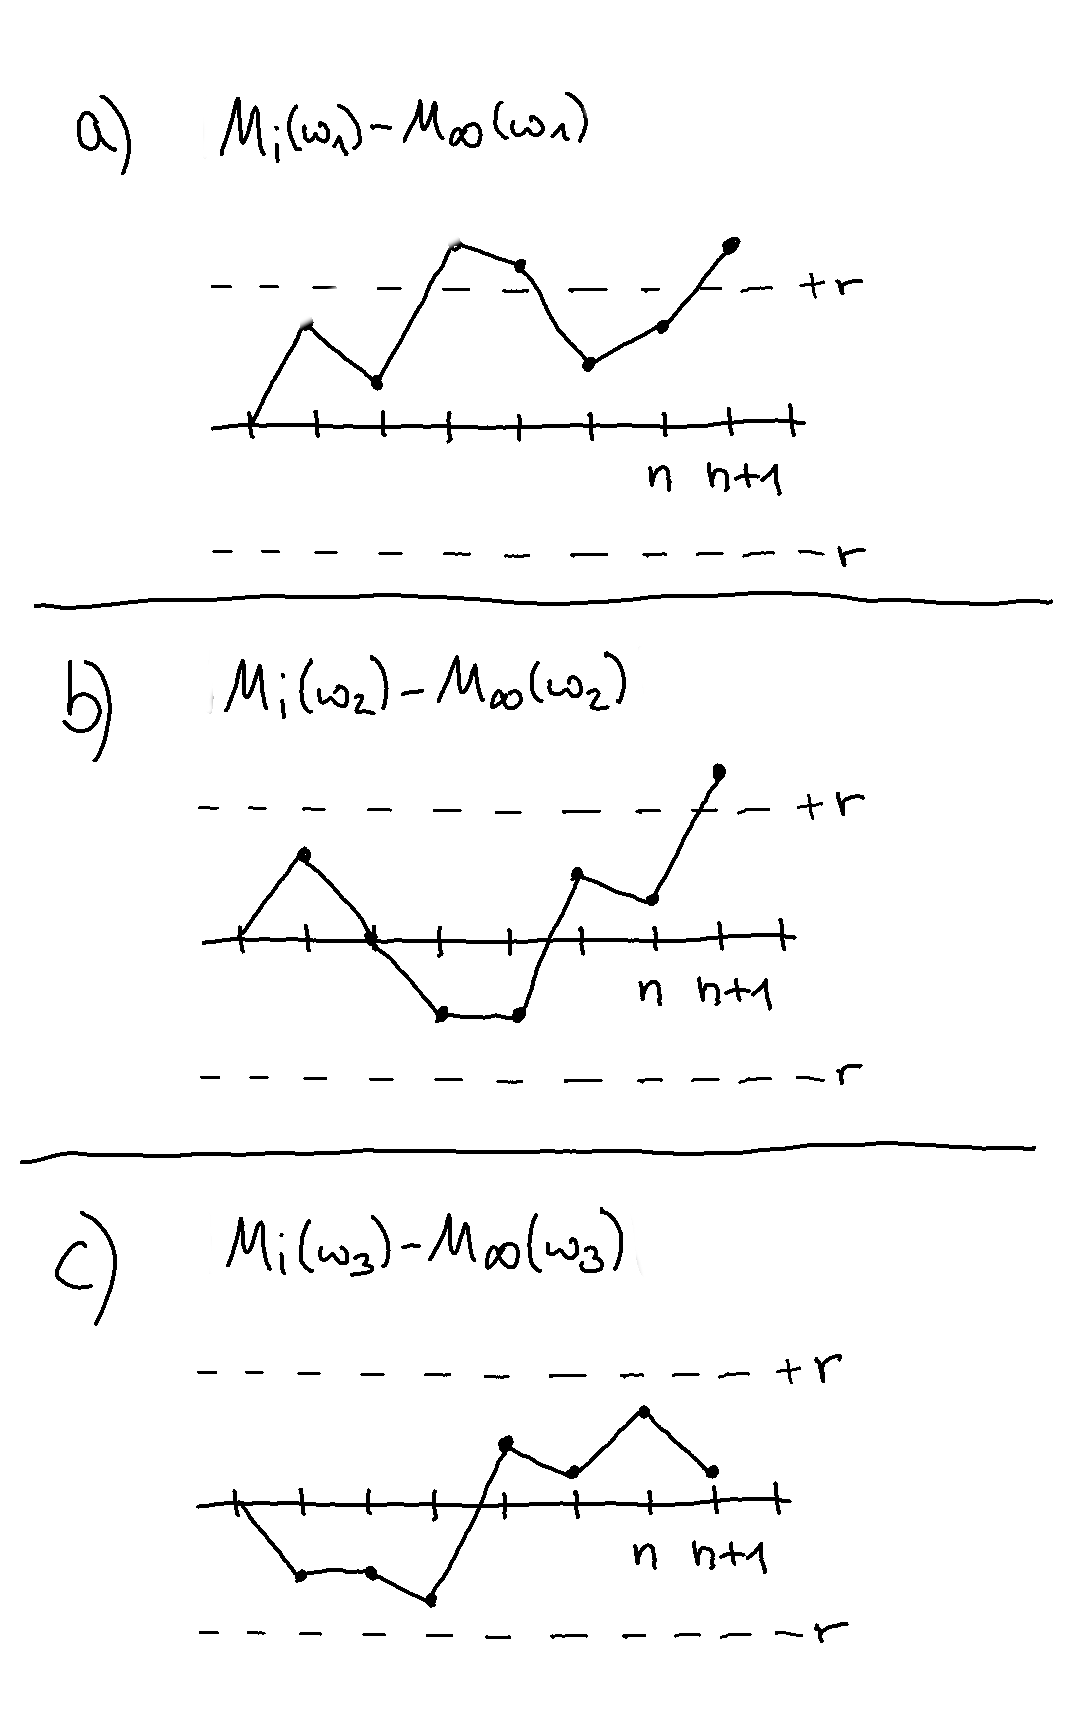
\includegraphics[width=0.65\textwidth]{\pathPrefix pics/SketchUE1.png}
		\begin{enumerate}[label=Fall \alph{*})]
			\item \qquad $\omega_1 \in A_n \quad \rightarrow\quad \omega_1 \in A_{n+1}$
			\item \qquad $\omega_2 \not\in A_n \quad \rightarrow \quad \omega_2 \in A_{n+1}$
			\item \qquad $\omega_3 \not\in A_n \quad \rightarrow \quad \omega_3 \not\in A_{n+1}$
		\end{enumerate}
		$\omega \in A_n \quad \rightarrow \quad \omega \not\in A_{n+1} \quad$ nicht möglich $\implies A_n \subset A_{n+1} \quad\forall n\in\N$
		\label{AbbUEProzess}
	\end{center}
\end{figure}

\begin{proof}[Beweis vom Professor]\enter
	$|M_n|$ ist Submartingal. Aus 4.2 folgt:
	\begin{align*}
		\exists M_\infty\in L_1:\P\left(\limn M_n=M_\infty\right)=1
	\end{align*}
	Mit Fatou kann man zeigen:
	\begin{align*}
		\E\Big[|M_\infty|^p\Big]
		&=\E\left[\limn |M_n|^p\right]
		\overset{\text{Fatou}}{\leq}
		\liminf\limits_{n\to\infty}\E\Big[|M_n|^p\Big]\leq B<\infty\\
		&\implies M_\infty\in L_p
	\end{align*}
	Jetzt nutzen wir majorierte Konvergenz:
	\begin{align*}
		\big|M_n-M_\infty\big|^p
		&\leq
		2^{p-1}\cdot\Big(|M_n|^p+|M_\infty|^p\Big)\\
		&\leq 2^{p-1}\cdot\Bigg(\left(\sup\limits_{n\in\N_0}|M_n|\right)^p+\underbrace{|M_\infty|^p}_{\text{integrierbar}}\Bigg)
	\end{align*}
	Mit Doobs $L_p$-Ungleichung folgt:
	\begin{align*}
		\left\Vert\sup\limits_{0\leq n\leq N}|M_n|\right\Vert_p
		&\leq \frac{p}{p-1}\cdot\Vert M_n\Vert_p\leq B\\
		\implies
		\left\Vert\sup\limits_{0\leq n\leq N}|M_n|\right\Vert_p
		&\leq B<\infty
	\end{align*}
	d.h. $|M_n-M_\infty|^p$ ist integrierbare obere Schranke. Folglich:
	\begin{align*}
		\limn\E\left[|M_n-M_\infty|^p\right]	
		\overset{\text{domKonv}}=
		\E\left[\limn|M_n-M_\infty|^p\right]=0
	\end{align*}
\end{proof}


% This work is licensed under the Creative Commons
% Attribution-NonCommercial-ShareAlike 4.0 International License. To view a copy
% of this license, visit http://creativecommons.org/licenses/by-nc-sa/4.0/ or
% send a letter to Creative Commons, PO Box 1866, Mountain View, CA 94042, USA.

\section{Aufgabenblatt 4}
\subsection{Aufgabe 4.1 (Monotonie der klassischen Aussagenlogik)}
Seien $G$ aussagenlogische Formel und seien $\F$ und $\F'$
Mengen aussagenlogischer Formeln. 
Dann gilt:
\begin{align*}
	\big(\F\models G\und \F\subseteq\F'\big)\implies\F'\models\F
\end{align*}
Erinnerung:
\begin{align*}
	\F'\models G:\Longleftrightarrow\big(\forall I:I\models\F'\implies I\models G\big)
\end{align*}

\begin{proof}
	Sei also $I$ beliebige Interpretation mit $I\models\F'$. 
	Dann gilt nach Definition
	\begin{align*}
		\forall F'\in\F':I\models F'
	\end{align*}
	Da $\F\stackrel{\text{Vor}}{\subseteq}\F'$ folgt 
	\begin{align*}
		\forall F\in\F:I\models F
	\end{align*}
	Aus der Voraussetzung $\F\models G$ folgt nun $I\models G$. 
	Da die Interpretation $I$ beliebig war, folgt die Behauptung $\F'\models G$. 
\end{proof}

\subsection{Aufgabe 4.2  (Wissenswertes über Nessie)}
\subsubsection{Aufgabe 4.2 (a)}
\begin{align*}
	F_1 &=(m \to\neg s)\\
	F_2 &=(\neg m\to (s\wedge t))\\
	F_3&=((\neg s\vee t)\to d)\\
	F_4&=(d\to a)
\end{align*}

\subsubsection{Aufgabe 4.2 (b)}
Wissen über Nessie ist $\F:=\lbrace F_1,\ldots, F_4\rbrace$.
``Folgt daraus, dass Nessie ein Märchenwesen ist?'', d. h.
Frage: Gilt $\F\models m$?

\begin{lösung}
	Man könnte an dieser Stelle \textit{Resolution} verwenden, aber es geht auch naiv. 
	Betrachte die Interpretation $I_1$ mit\\
	$m^{I_1}=\top,~s^{I_1}=\bot,~d^{I_1}=\top,~a^{I_1}=\top$ und $t^{I_1}$ beliebig\\ und die Interpretation $I_2$ mit\\
	$m^{I_2}=\bot,~s^{I_2}=\bot,~t^{I_2}=\top, d^{I_2}=\top,a^{I_2}=\top$\\
	Dann gilt $I_1\models\F$ und $I_2\models\F$ aber $I_1\models m$ und $I_2\not\models m$. 
	Also folgt $F\not\models m$ und $\F\not\models\neg m$.
	Man kann also nichts folgern.
\end{lösung}

\subsection{Aufgabe 4.3 (Logische Äquivalenzen)}
Beachte zunächst
\begin{align*}
	G\equiv F &\stackrel{\text{Def}}{\Longleftrightarrow}
	\Big(\forall I:I\models F\gdw I\models G\Big)\\
	\overset{\text{Def}}&{\Longleftrightarrow}
	\Big(\forall I:G^I=\top\gdw F^I=\top\Big)\\
	&\Longleftrightarrow\forall I:F^I=G^I
\end{align*}

Sei also $I$ eine beliebige Interpretation im Folgenden.

\subsubsection{Aufgabe 4.3 (a)}
\begin{align*}
	[(F\vee F)]^I=F^I\vee^\ast F^I\stackeq{\text{Tab}} F^I
\end{align*}
\begin{tabular}{c||c}
	$F^I$ & $F^I\vee^\ast F^I$\\ \hline
	$\top$ & $\top$\\
	$\bot$ & $\bot$
\end{tabular}

\subsubsection{Aufgabe 4.3 (b)}
\begin{align*}
	[\neg(F\wedge G)]^I=\neg^\ast\left(F^I\wedge^\ast G^I\right)\stackeq{\text{Tab}}
	\left(\neg^\ast F^I\vee^\ast\neg^\ast G^I\right)=\big[(\neg F\vee\neg G)\big]^I
\end{align*}

\begin{tabular}{c|c||c|c}
	$F^I$ & $G^I$ & $\neg^\ast(F^I\wedge^\ast G^I)$ & $(\neg^\ast F^I\vee^\ast\neg^\ast G^I)$\\ \hline
	$\top$ & $\top$ & $\bot$ & $\bot$\\
	$\top$ & $\bot$ & $\top$ & $\top$\\
	$\bot$ & $\top$ & $\top$ & $\top$\\
	$\bot$ & $\bot$ & $\top$ & $\top$
\end{tabular}

\subsubsection{Aufgabe 4.3 (c)}
Analog zu (a) und (b).
%\begin{align*}
%[(F\to G)]^I=\left(F^I\to^\ast G^I\right)\stackeq{\text{Tab}}
%\left( F^I\to^\ast\neg^\ast G^I\right)=\big[(\neg F\vee\neg G)\big]
%\end{align*}

\subsubsection{Aufgabe 4.3 (d)}
Analog zu (a) und (b).

\subsubsection{Aufgabe 4.3 (e)}
Analog zu (a) und (b).

\subsubsection{Aufgabe 4.3 (f)}
Analog zu (a) und (b).

\subsubsection{Aufgabe 4.3 (g)}
Analog zu (a) und (b).

\subsection{Aufgabe 4.4 (Das vollständige Junktorensystem \texorpdfstring{$\lbrace\neg, \vee\rbrace$}{lbrace neg,vee rbrace})}
Zeigen Sie: Es gibt zu jeder aussagenlogischen Formel (mit was auch immer für ein-und zweistelligen Junktoren aus dem Reservoir der 4 bzw. 16 möglichen Junktoren) eine
semantisch äquivalente Formel, welche nur die Junktoren $\neg$ und $\vee$ enthält.

\begin{lösung}
	Sei $\mathcal{R}=\lbrace p_1,p_2,\ldots\rbrace$ eine Menge von aussagenlogischen Variablen, 
	$J_1:=\lbrace J_1^1,\ldots,J_1^4\rbrace$ die Menge der einstelligen Junktoren und $J_2:=\lbrace J_2^1,\ldots,J_2^{16}\rbrace$ die Menge der zweistelligen Junktoren. 
	(Es gibt nach Vorlesung genau 4 einstellige und 16 zweistellige Junktoren). 
	Es müssen also zunächst folgende 16 + 4 Ersetzungsrelegung bzw. semantische Äquivalenzen gezeigt werden (analog zu Aufgabe 4.3):
	\begin{enumerate}
		\item $J_1^1 A\equiv\neg A$
		\item $J_1^2 A\equiv\neg\neg A$
		\item $J_1^3 A\equiv A\vee\neg A$
		\item $J_1^4 A\equiv\neg(A\vee\neg A)$
	\end{enumerate}
	und
	\begin{enumerate}
		\item $A J_2^1 B\equiv A\vee B$
		\item $A J_2^2 B=A\wedge B\equiv\neg(\neg A\vee\neg B)$
		\item $A J_2^3 B=A\to B\equiv\neg A\vee B$
		\item $\ldots$
	\end{enumerate}
	Nun können wir eine rekursive Funktion auf der Menge der Formeln über den 16+4 Junktoren definieren.
	Diese konkret aufzuschreiben ist etwas awkward und wird hier nicht gemacht.
\end{lösung}

\textbf{Mitschrift aus der Übung:}
\begin{lösung}
	Leite für jeden Junktor aus der Wahrheitswertetabelle eine äquivalente Formel und daraus dann eine Ersetzungsregel ab. 
	Dabei nutzen wir die de'Morgansche Regel:
	\begin{align*}
		(\varphi_1\wedge\varphi_2)\equiv\neg(\neg\varphi_1\vee\neg\varphi_2)
	\end{align*}
	Daraus erhält man die Ersetzungsregel
	\begin{align}\label{4.4Ersetzungsregel}
		\frac{(\varphi_1\wedge\varphi_2)}{\neg(\neg\varphi_1\vee\neg\varphi_2)}
	\end{align}
	Hier am Beispiel der Implikation:\\
	\begin{tabular}{c|c||c}
		$\varphi_1^I$ & $\varphi_2^I$ & $\varphi_1^I\to^\ast\varphi_2^I$ \\ \hline
		$\top$ & $\top$ & $\top$\\
		$\top$ & $\bot$ & $\bot$\\
		$\bot$ & $\top$ & $\top$\\
		$\bot$ & $\bot$ & $\top$
	\end{tabular}

	\begin{align*}
		(\varphi_1\to\varphi_2)
		&\equiv (\varphi_1\wedge\varphi_2)\vee(\neg\varphi_1\wedge\varphi_2)\vee(\neg\varphi_1\wedge\neg\varphi_2)\\
		\overset{\eqref{4.4Ersetzungsregel}}&{\equiv}
		\neg(\neg\varphi_1\vee\neg\varphi_2)\vee\neg(\neg\neg\varphi_1\vee\varphi_2)\vee\neg(\neg\neg\varphi_1\vee\neg\neg\varphi_2)\\
		&\equiv(\neg\varphi_1\vee\varphi_2)
	\end{align*}
	Somit erhält man die Ersetzungsregel
	\begin{align*}
		\frac{(\varphi_1\to\varphi_2)}{(\neg\varphi_1\vee\varphi_2)}
	\end{align*}
	Erhalte somit alle 16 + 4 Ersetzungsregel erschöpfend auf die Formel an (d.h. bis keine Ersetzungsregel mehr anwendbar ist). 
	Damit erhält man nach endlich vielen Schritten eine semantisch äquivalente Formel, welche nur noch $\neg$ und $\vee$ enthält.
\end{lösung}

\subsection{Aufgabe 4.5 (Positionen und Ersetzungen in Formeln)}
\subsubsection{Aufgabe 4.5 (a)}
\begin{tikzpicture}[node distance=5em]
	\tikzstyle{every state}=[shape=circle,draw=black]
	\node[state] (1) {$\neg:\Lambda$};
	\node[state] (2) [below = of 1] {$\wedge:1$};
	\node[state] (3) [below left = of 2] {$p:11$};
	\node[state] (4) [below right = of 2] {$\vee:12$};
	\node[state] (5) [below left = of 4] {$q:121$};
	\node[state] (6) [below right = of 4] {$\neg:122$};
	\node[state] (7) [below of =6] {$p:1221$};
	\path 	(2) edge [, -] node {} (1)
   	   		(3) edge [, -] node {} (2)
		 	(4) edge [, -] node {} (2)
	  		(5) edge [, -] node {} (4)
	 		(6) edge [, -] node {} (4)
	  		(7) edge [, -] node {} (6)
	;	
\end{tikzpicture}

\begin{align*}
	\mathcal{P}_F=\lbrace\Lambda,1,11,12,121,122,1221\rbrace
\end{align*}
Formal:
\begin{align*}
	\pos(\neg(p\wedge(q\vee\neg p)))
	\overset{2.}&=
	\lbrace\Lambda\rbrace\cup\lbrace 1\pi:\pi\in\pos((p\wedge(q\vee\neg p)))\rbrace\\
	&=\lbrace\Lambda,1\Lambda,11\Lambda,12\Lambda,121\Lambda,122\Lambda,1221\Lambda\rbrace\\
	\pos((p\wedge(q\vee\neg p)))
	\overset{3}&=
	\lbrace\Lambda\rbrace\cup\lbrace 1\pi_1:\pi_1\in\pos(p)\rbrace\cup\lbrace 2\pi_2:\pi_2\in\pos((q\vee\neg p))\rbrace\\
	&=\lbrace\Lambda,1\Lambda,2\Lambda,21\Lambda,22\Lambda,221\Lambda\rbrace\\
	\pos(p)&\stackeq{1.}\lbrace\Lambda\rbrace\cup\emptyset=\lbrace\Lambda\rbrace\\
	\pos((q\vee\neg p))&\stackeq{3.}\lbrace\Lambda\rbrace\cup\lbrace1\pi_1:\pi_1\in\pos(q)\rbrace\cup\lbrace 2\pi_2:\pi_2\in\pos(\neg p)\rbrace\\
	&=\lbrace\Lambda,1\Lambda,2\Lambda,21\Lambda\rbrace\\
	\pos(q)&\stackeq{1.}\lbrace\Lambda\rbrace\cup\emptyset=\lbrace\Lambda\rbrace\\
	\pos(\neg p)&\stackeq{2.}\lbrace\Lambda\rbrace\cup\lbrace 1\pi:\pi\in\pos(p)\rbrace=\Lambda,1\Lambda\rbrace
\end{align*}

\subsubsection{Aufgabe 4.5 (b)}
\begin{tikzpicture}[node distance=5em]
	\tikzstyle{every state}=[shape=circle,draw=black]
	\node[state] (1) {$\neg:\Lambda$};
	\node[state] (2) [below = of 1] {$\neg:1$};
	\node[state] (3) [below = of 2] {$\wedge:11$};
	\node[state] (4) [left = of 3] {$\vee:111$};
	\node[state] (5) [below left = of 4] {$p:1111$};
	\node[state] (6) [below right = of 4] {$q:1112$};
	\node[state] (7) [right = of 3] {$\vee:112$};
	\node[state] (8) [below left = of 7] {$q:1121$};
	\node[state] (9) [below right = of 7] {$\neg:1122$};
	\node[state] (10) [below = of 9] {$p:11221$};
	\path 	(2) edge [, -] node {} (1)
      		(3) edge [, -] node {} (2)
	  		(4) edge [, -] node {} (3)
	  		(5) edge [, -] node {} (4)
	  		(6) edge [, -] node {} (4)
	  		(7) edge [, -] node {} (3)
	  		(8) edge [, -] node {} (7)
	  		(9) edge [, -] node {} (7)
	  		(10) edge [, -] node {} (9)
	;	
\end{tikzpicture}

\begin{align*}
	G\lceil 1122\Lambda\rceil
	&=\Big[\neg\neg((p\vee q)\wedge(q\vee\neg p))\Big]\lceil 1122\Lambda\rceil\\
	&\stackeq{\text{2.}}
	\Big[\neg((p\vee q)\wedge(q\vee\neg p))\Big]\lceil 122\Lambda\rceil\\
	&\stackeq{\text{2.}}
	\Big[((p\vee q)\wedge(q\vee\neg p))\Big] \lceil 22\Lambda\rceil\\
	&\stackeq{\text{3.}}
	\Big[(q\vee\neg p)\Big]\lceil 2\Lambda\rceil\\
	&\stackeq{\text{3.}}
	[\neg p]\lceil\Lambda\rceil\\
	&\stackeq{\text{1.}}[\neg p]=\neg p
\end{align*}

\subsubsection{Aufgabe 4.5 (c)}
\begin{tikzpicture}[node distance=3em]
	\tikzstyle{every state}=[shape=circle,draw=black]
	\node[state] (1) {$\neg:\Lambda$};
	\node[state] (2) [below = of 1] {$\wedge:1$};
	\node[state] (3) [below left = of 2] {$\neg:11$};
	\node[state] (4) [below left = of 3] {$\vee:111$};
	\node[state] (5) [below left = of 4] {$p:1111$};
	\node[state] (6) [below right= of 4] {$q:1112$};
	\node[state] (7) [below right = of 2] {$\neg:12$};
	\node[state] (8) [below right = of 7] {$\vee:121$};
	\node[state] (9) [below left = of 8] {$q:1211$};
	\node[state] (10) [below right = of 8] {$\neg:1212$};
	\node[state] (11) [below = of 10] {$p:12121$};
	\path 	(2) edge [, -] node {} (1)
   		   	(3) edge [, -] node {} (2)
	  		(4) edge [, -] node {} (3)
	  		(5) edge [, -] node {} (4)
	  		(6) edge [, -] node {} (4)
	  		(7) edge [, -] node {} (2)
	  		(8) edge [, -] node {} (7)
	  		(9) edge [, -] node {} (8)
	  		(10) edge [, -] node {} (8)
	  		(11) edge [, -] node {} (10)
		;	
\end{tikzpicture}

\begin{align*}
	H\Big\lceil 121\Lambda\mapsto(\neg p\to q)\Big\rceil
	&=
	\Big[\neg(\neg(p\vee q)\wedge\neg(q\vee\neg p))\Big]\Big\lceil 121\Lambda\mapsto(\neg p\to q)\Big\rceil\\
	&\stackeq{\text{2.}}
	\neg\Big[(\neg(p\vee q)\wedge\neg(q\vee\neg p))\Big]\Big\lceil 21\Lambda\mapsto(\neg p\to q)\Big\rceil\\
	&\stackeq{\text{4.}}
	\neg\Big(\neg(p\vee q)\wedge\Big[\neg(q\vee\neg p)\Big]\Big\lceil 1\Lambda\mapsto(\neg p\to q)\Big\rceil\Big)\\
	&\stackeq{\text{2.}}
	\neg\Big(\neg(p\vee q)\wedge\neg\Big[(q\vee\neg p)\Big]\Big\lceil\Lambda\mapsto(\neg p\to q)\Big\rceil\Big)\\
	&\stackeq{\text{1.}}
	\neg\Big(\neg(p\vee q)\wedge\neg(\neg p\to q)\Big)
\end{align*}
Zur semantischen Äquivalenz: Das Ersetzungstheorem (Satz 3.23) ist nicht anwendbar, da 
\begin{align*}
	(q\vee\neg p)\not\equiv(\neg p\to q)
\end{align*}
Tatsächlich gilt
\begin{align*}
	H\not\equiv H\lceil 121\mapsto(\neg p\to q)\rceil
\end{align*}
Betrachte die Interpretation $I$ mit $p^I=q^I=\bot$.

\subsection{Aufgabe 4.6 (Formelersetzungen)}
\subsubsection{Aufgabe 4.6 (a)}
Die Aussage gilt nicht, denn betrachte folgendes Gegenbeispiel:\\
$F=(p\wedge p)=p\vee G$ mit $\pi=1$ und $H=\neg p$. 
Dann sind $F,G,H$ erfüllbar aber \\
$F\lceil\pi\to H\rceil=(p\vee\neg p)$ ist unerfüllbar.\\
Also: Obwohl die Formeln $F,G,H$ unabhängig voneinander erfüllbar sind, können in $H$ Variablen verwendet werden, die auch an anderer Stelle in $F$ vorkommen.

\subsubsection{Aufgabe 4.6 (b)}
Die Aussage stimmt, denn:\\
Durch scharfes Hinsehen (oder Wahrheitswertetabelle) sieht man (aufgrund der Unerfüllbarkeit von $G$)
\begin{align*}
	G\equiv((H\wedge G)\wedge(H\vee G))
\end{align*}
Nach dem Ersetzungstheorem (Satz 3.23) folgt damit die Behauptung, da in $F$ eine Teilformel durch eine semantisch äquivalente Formel ersetzt wird.

\subsubsection{Aufgabe 4.6 (c)}
Die Aussage stimmt nicht. Betrachte\\
$F=\neg p,\pi=1\Lambda,G=p,H=(p\vee q)$, offensichtlich ist $G\to H$ eine Tautologie, aber $F\to F\lceil\pi\mapsto H\rceil=\neg p\to\neg(p\vee q)$ nicht allgemeingültig. Denn $p^I=\bot$, $q^I=\top$)

%$G=H=p\wedge\neg p$ und $F=\neg H$ mit $\pi=\Lambda$. Dann ist $H\to G$ allgemeingültig, aber
%$F\to \underbrace{F\lceil\pi\to G\rceil}_{=H}$ ist unerfüllbar, denn $F$ ist allgemeingültig und $H$ unerfüllbar.\\


% This work is licensed under the Creative Commons
% Attribution-NonCommercial-ShareAlike 4.0 International License. To view a copy
% of this license, visit http://creativecommons.org/licenses/by-nc-sa/4.0/ or
% send a letter to Creative Commons, PO Box 1866, Mountain View, CA 94042, USA.
% vim: set noexpandtab:

\section{Aufgabenblatt 5}
\subsection{Aufgabe 5.1}
Sei $K=(a,a+h)$ mit $a\in\R$ und $h>0$ ein offenes Intervall.

\subsubsection{Aufgabe 5.1 (a)}
Es gilt für alle $v\in P_k(K)$ und $0\leq m\leq l$ sowie $p,q\in[1,\infty]$ die inverse Ungleichung
\begin{align*}
	|v|_{l,p,K}\leq c\cdot h^{m-l+\left(\frac{1}{p}-\frac{1}{q}\right)}\cdot|v|_{m,q,K}
\end{align*}
wobei $C$ eine Konstante ist, die nicht von $K$ abhängt (und damit insbesondere auch nicht von $h$).

\begin{proof}
	%Nutze Transformation auf Referenzelement $\hat{K}=(0,1)$, also
	%\begin{align*}
		%f:\R\to\R,\qquad x\mapsto h\cdot x+a
	%\end{align*}
	In Aufgabe 4.5 haben wir gezeigt für $\hat{K}=(0,1)$:
	\begin{align*}
		|\hat{v}|_{m,p,\hat{K}}\leq h^m\cdot\left(\frac{1}{h}\right)^{\frac{1}{p}}\cdot|v|_{m,p,K}
	\end{align*}
	Damit folgt:
	\begin{align*}
		|v|_{l,p,K}
		&=\underbrace{h^{-l}\cdot\left(\frac{1}{h}\right)^{-\frac{1}{p}}}_{=h^{-l+\frac{1}{p}}}\cdot\underbrace{|\hat{v}|_{l,p,\hat{K}}}_{\stackrel{l\geq m}{\leq}\Vert \hat{v}^{(m)}\Vert_{l-m,p,\hat{K}}}
	\end{align*}
	Jetzt nutzen wir die Äquivalenz der Normen auf dem endlich dimensionalem Raum $P_k(\hat{K})$:
	\begin{align*}
		\Vert \hat{v}^{(m)}\Vert_{l-m,p,\hat{K}}
		&\leq
		c\cdot\underbrace{\Vert\hat{v}^{(m)}\Vert_{0,q,\hat{K}}}_{=|\hat{v}|_{m,q,\hat{K}}}
	\end{align*}
	wobei $c$ unabhängig von $h(K)$ ist wegen des Referenzelements $\hat{K}$. Folglich gilt:
	\begin{align*}
		|v|_{l,p,K}
		&\leq
		c\cdot h^{-l+\frac{1}{p}}\cdot\underbrace{|\hat{v}|_{m,q,\hat{K}}}_{\stackeq{\text{Aufg. 4.5}}h^{k-\frac{1}{q}}\cdot|v|_{m,q,\hat{K}}}
		=c\cdot h^{m-l+\left(\frac{1}{p}-\frac{1}{q}\right)}\cdot|v|_{m,q,K}
	\end{align*}
	%Es gilt
	%\begin{align*}
		%\min\limits_{p\in P_k}\big\Vert\hat{v}+p\big\Vert_{0,p,\hat{K}}\leq c\cdot|\hat{v}|_{k+1,p,\hat{K}}
	%\end{align*}
\end{proof}

\begin{bemerkung}
	Falls $v$ eine Funktion auf einen Finiten-Elemente-Raum (also endlich dimensional) ist, das Element $(K,V,\Sigma)$ von der Triangulierung affin äquivalent zum Referenzelement $(\hat{K},\hat{V},\hat{\Sigma})$ ist, dann gilt:
	\begin{align*}
		\Vert v\Vert_{l,p,K}\leq c\cdot h_K^m\cdot\rho_k^{-l}\cdot\meas(K)^{\frac{1}{p}-\frac{1}{q}}\cdot\Vert v\Vert_{m,q,K}
	\end{align*}
	Falls $n$ die Dimension notiert, dann gilt:
	\begin{align*}
		c\cdot \rho_k^n&\leq\meas(K)\leq c\cdot h_k^n\\
		\frac{h_k}{\rho_k}&\leq c\qquad\text{(form-regulär)}\\
		\implies\Vert v\Vert_{l,p,K}&\leq c\cdot h_K^{m-l+n\cdot\left(\frac{1}{p}-\frac{1}{q}\right)}\cdot\Vert v\Vert_{m,q,K}\\
		\Vert v\Vert_{l,p,K}&=\sum\limits_{i=}^{m+1}\big| v^{(i)}\big|_{0,p,K}+\big\Vert v^{(m)}\big\Vert_{l-m,p,K}
	\end{align*}
	Rest der Lösung steht online.
	% login: PDENM18, PW: weak
\end{bemerkung}

$V_h\subseteq V$ ist konform mit $V\subseteq H^1(\Omega)\hookrightarrow C(\Omega)$\\
$V_h\not\subseteq V$ ist nichtkonform.

\subsubsection{Aufgabe 5.1 (b)}
Wie muss die rechte Seite angepasst werden, wenn die volle $W^{l,p}$-Norm in ähnlicher Weise abgeschätzt werden soll?

\begin{lösung}
	%TODO
\end{lösung}

\subsection{Aufgabe 5.2}
Im Rahmen nichtkonformer Finite Elemente soll die folgende Verallgemeinerung des Dualitätsarguments von Aubin-Nitsche untersucht werden.\\
Sei $H$ ein Hilbertraum mit Norm $\Vert\cdot\Vert_H$ und Skalarprodukt $(\cdot,\cdot)$. 
Ferner sei $V_h\subseteq H$ abgeschlossen mit Norm $\Vert\cdot\Vert_h$ und $V$ ein Hilbertraum, welcher stetig in $H$ eingebettet ist $(V\hookrightarrow H$). 
Die auf $V+V_h$ definierte und stetige Bilinearform $a_h$ stimme auf $V$ mit $a$ überein. 
Dann gilt:
\begin{align*}
	\Vert u-u_h\Vert_H\leq\sup\limits_{g\in H\setminus\lbrace0\rbrace}\frac{1}{\Vert g\Vert_H}\cdot\Big( &M\cdot\Vert u-u_h\Vert_h\cdot\Vert\varphi_g-\varphi_{g,h}\Vert_h\\
	&+\big|a_h(u-u_h,\varphi_g)-(u-u_h,g)\big|\\
	&+\big|a_h(u,\varphi_g-\varphi_{g,h})-(f,\varphi_g-\varphi_{g,h})\big|\Big)
\end{align*}
wobei zu $g\in H$ die Funktionen $\varphi_g\in V$ und $\varphi_{g,h}\in V_h$ als Lösungen von
\begin{align*}
	a(w,\varphi_g)=(w,g)\quad\forall w\in V\qquad\text{bzw.}\qquad a_h(w_h,\varphi_{g,h})=(w_h,g)\quad\forall w_h\in V_h
\end{align*}
definiert sind.

\begin{proof}
	Auf $V\times V$ gilt $a=a_h$
	\begin{align*}
		a_h:(V+V_h)\times(V+V_h),\qquad
		a(u,v)&=\int\limits_\Omega\nabla u\cdot\nabla v\d x\\
		a_h(u,v)&=\sum\limits_{K}\int\limits_K\nabla u\cdot\nabla v\d x
	\end{align*}
	Setze $\varphi_h:=\varphi_{g,h}$. Dann gilt:
	\begin{align*}
		(u-u_h,g)&=a(\underbrace{u}_{\in V},\underbrace{\varphi_g}_{\in V})-a_h(u_h,\varphi_h)\\
		&=a_h(u,\varphi_g)-a_h(u_h,\varphi_h)\\
		&=a_h(u,\varphi_g\underbrace{-\varphi_h)+a_h(u,\varphi_h)}_{=0}-a_h(u_h,\varphi_h)\\
		&{} \quad-\underbrace{a_h(u_h,\varphi_g-\varphi_h)+a_h(u_h,\varphi_g-\varphi_h)}_{=0}\\
		&=a_h(u-u_h,\varphi_g-\varphi_h)+\underbrace{a_h(u-u_h,\varphi_h)}_{(1)}+\underbrace{a_h(u_h,u_g-\varphi_h)}_{(2)}
	\end{align*}
	%TODO hier fehlt was
	und außerdem
	\begin{align*}
		a_h(u,\varphi_g-\varphi_h)-(f,\varphi_g-\varphi_h)
		&=\underbrace{a_h(u,\varphi_g)-(f,\varphi_g)}_{=0, \text{weak solution}}-a_h(u,\varphi_h)+\underbrace{(f,\varphi_h)}_{\stackeq{\text{Def }u_h}a_h(u_h,\varphi_h)}\\
		&=-a_h(u-u_h,\varphi_h) = (1)
	\end{align*}
	und außerdem %Wortwiederholung als Ausdruck von Langeweile
	\begin{align*}
		a_h(u-u_h,\varphi_g)-(u-u_h,g)
		&=\underbrace{a(u,\varphi_g)-(u,g)}_{=0}-a_h(u_h,\varphi_g)+\underbrace{(u_h,g)}_{=a_h(u_h,\varphi_h)}\\
		&=-a_h(u_h,\varphi_g-\varphi_h) = -(2)
	\end{align*}
	und außerdem %Wortwiederholung als Ausdruck von Langeweile
	\begin{align*}
		\Vert u-u_h\Vert
		&=\sup\limits_{g\in H\setminus\lbrace0\rbrace}\frac{(u-u_h,g)}{\Vert g\Vert_H}
	\end{align*}
	Damit folgt mit der Stetigkeit von $a_h$ und dem Betrag auf der rechten Seite die Behauptung.
\end{proof}

\subsection{Aufgabe 5.3}
Sei $\Omega$ ein konvexes Polyeder. Beweisen Sie für die Diskretisierung der Poisson-Gleichung
\begin{align*}
	\left\lbrace\begin{array}{rl}
		-\Delta u=f &\text{ in }\Omega\\
		u|_{\partial\Omega}=0
	\end{array}\right.\mit f\in L^2(\Omega)
\end{align*}
mit Crouzeix-Raviart-Elementen über einer regulären Zerlegung von $\Omega$ die \\$L^2$-Fehlerabschätzung
\begin{align*}
	\Vert u-u_h\Vert_0\leq c\cdot h^2\cdot\Vert u\Vert_2
\end{align*}

\begin{proof}
	$V=H_0^1(\Omega)$, $H=L^2$, $V_h\not\subseteq V$
	\begin{align*}
		a(v,w)&=\int\limits_\Omega\nabla v\cdot\nabla w\d x\\
		a_h(v,w)&=\sum\limits_K\int\limits_K\nabla v\cdot\nabla w\d x
	\end{align*}

	\underline{Teilschritt (a):}\\
	Das Dualitätsargument von Aubin-Nitsche ist anwendbar (klar).\nl
	\underline{Teilschritt (b):}\\
	Aus der Vorlesung ist bekannt:
	\begin{align*}
		\Vert u-u_h\Vert_h\leq c\cdot h\cdot\Vert u\Vert_2
	\end{align*}
	Bei der Abschätzung von $\Vert\varphi_g-\varphi_{g,h}\Vert$ hilft, dass $\varphi_g-\varphi_{g,h}$ als Diskretisierungsfehler des Problems 
	$a(w,\varphi)=(w,g)$ angesehen werden kann.\nl
	$\varphi_g$ und $\varphi_{g,h}$ sind auch schwache und diskrete Lösungen der Poisson-Gleichung, aber mit rechter Seite $g$ anstelle von $f$. 
	Folglich kann die Abschätzung aus der Vorlesung benutzt werden und es gilt
	\begin{align*}
		\Vert\varphi_g-\varphi_{g,h}\Vert_h\leq c\cdot h\cdot\Vert\varphi_g\Vert_2
	\end{align*}

	\underline{Teilschritt (c):}\\
	Es ist bekannt:
	\begin{align*}
		\big|L_w(z)\big|:=\Big|a_h(w,z)-(\hat{f},z)\Big|\leq c\cdot h\cdot\Vert w\Vert_2\cdot\Vert z\Vert_h\qquad\forall z\in V_h+v,\forall w\in H^2
	\end{align*}
	und $w$ erfüllt die Gleichung $-\Delta w = \hat{f}$.%f_{snake}%\~{f}$
	Dann folgt:
	\begin{align*}
		\underbrace{\big|a_h(u-u_h,\varphi_g)-(u-u_h,g)\big|}_{=|L_{\varphi_g}(u-u_h)|} &\leq Ch \|\varphi_g\|_2\underbrace{\|u-u_h\|_h}_{Ch\|u\|_2}\\
		&\leq Ch^2 \|u\|_2\|\varphi_g\|_2
	\end{align*}
	und
	\begin{align*}
		\underbrace{\big|a_h(u,\varphi_g-\varphi_{g,h})-(f,\varphi_g-\varphi_{g,h})\big|}_{=|L_{u}(\varphi_g-\varphi_{g,h})|} &\leq Ch \|u\|_2\underbrace{\|\varphi_g - \varphi_{g,h}\|_h}_{Ch\|\varphi_g\|_2} \\
		&\leq Ch^2 \|u\|_2\|\varphi_g\|_2
	\end{align*}

	%TODO vermutlich fehlt hier auch was. Bin dermaßen raus, dass ich das nicht einmal mehr einschätzen kann xD Haha 

	\underline{Teilschritt (d):}
	\begin{align*}
		\Vert u-u_h\Vert_0\leq\sup\limits_{g\in H\setminus\lbrace0\rbrace}\frac{1}{\Vert g\Vert_H}\big\lbrace(\text{MC+CC})~h^2\cdot\Vert u\Vert_2\cdot\underbrace{\Vert\varphi_g\Vert_2}_{C\|g\|_H}\big\rbrace
		\end{align*}
	Aus dem \textit{Regularitäts-Theorem} folgt, da $\Omega$ konvex ist ist:
	\begin{align*}
		\varphi_g\in H^2\qquad\text{und}\qquad\Vert\varphi_g\Vert_2\leq c\cdot\Vert g\Vert_0
	\end{align*}
	$\implies$ 
	\begin{align*}
		\|u-u_h\|_0 \leq C h^2 \|u\|_2.
	\end{align*}
	(Hier wird manchmal die $\|\cdot\|_0$-Norm verwendet. Diese soll anscheinend die $H$-Norm sein.)
\end{proof}

\subsection{Aufgabe 5.4}
	Sei $\Omega$ ein konvexes Polyeder. 
	Es erfülle $w\in H^2(\Omega)\cap H_0^1(\Omega)$ die Poisson-Gleichung $-\Delta w=\hat{f}$. 
	Ferner sei für $z\in V_h+V$
	\begin{align*}
		L_w(z):=a_h(w,z)-(\hat{f},z):=\sum\limits_K\int\limits_K\nabla w\cdot\nabla z\d x-\int\limits_\Omega\hat{f}\cdot z\d x
	\end{align*}
	wobei $V_h$ den Raum der Crouzeix-Raviart-Elemente über einer regulären Zerlegung von $\Omega$ bezeichne und $V=H_0^1(\Omega)$ sein.

\subsubsection{Aufgabe 5.4 (a)}
Es gilt
\begin{align*}
	L_w(z)=\sum\limits_K\sum\limits_{E\in\delta K}\int\limits_E\left(\frac{\partial}{\partial n_K}-\frac{\partial w^I}{\partial n_K}\right)\cdot\left(z-\overline{z(E)}\right)\d s
\end{align*}
Dabei bezeichne $w^I\in V_h\cap C^0(\Omega)$ die stetige, stückweise lineare Interpolierende, die $w$ in den Eckpunkten der Dreiecke interpoliert. 
Auf einer Kante $E$ sei
\begin{align*}
	\overline{z(E)}=\frac{1}{|E|}\cdot\int\limits_E z\d s
\end{align*}
der Integralmittelwert einer Funktion $z\in V_h+V$.

\subsubsection{Aufgabe 5.4 (b)}
Es gilt die Abschätzung
\begin{align*}
	\big|L_w(z)\big|\leq c\cdot h\cdot|w|_2\cdot\Vert z\Vert_h
\end{align*}

\begin{proof}
	Wir nutzen in dem Beweis die Spurungleichung in Kombination mit dem \\ Bramble-Hilbert-Lemma.
	%TODO
\end{proof}

% This work is licensed under the Creative Commons
% Attribution-NonCommercial-ShareAlike 4.0 International License. To view a copy
% of this license, visit http://creativecommons.org/licenses/by-nc-sa/4.0/ or
% send a letter to Creative Commons, PO Box 1866, Mountain View, CA 94042, USA.

\section{Aufgabenblatt 6}
\subsection{Aufgabe 6.1 (Resolutionsableitungen)}
Resolventenbildung: Entferne $A$ aus $C_1$ und $\neg A$ aus $C_2$ und verknüpfe den Rest disjunktiv.\\
Die Auswahl der beiden Klausel für die Resolventenbildung erfolgt mit der \textit{Methode des scharfen Hinsehens}. 
Es ist sinnvoll rückwärts zu denken:
\begin{align*}
	[A,B],[A,\neg B],[\neg A]\Reso[A,A],[\neg A]\Reso[~]
\end{align*}
Eine andere Strategie ist, zu Beginn alle einstelligen Klauseln auszunutzen. 
In Aufgabe 1 (b) kann man in allen Klauseln schon $\neg s$ und $r$ rausstreichen, wegen den Klauseln 4 und 5.

\subsubsection{Aufgabe 6.1}
\begin{align*}
	\begin{array}{rll}
		9 & \Res(2,6,t) & [q,r]\\
		10 & \Res(9, 7,r) & [q]\\
		11 & \Res(10,8,q) & [\neg t]\\
		12 & \Res(11,2, t) & [~]
	\end{array}
\end{align*}

\subsubsection{Aufgabe 6.2}
\begin{align*}
	\begin{array}{rll}
		9 & \Res(4,7,s) & [q,r]\\
		10 & \Res(5,9,r) & [q]\\
		11 & \Res(4,8,s) & [\neg q,\neg q]\\
		13 & \Res(10,11,q) & [~]
	\end{array}
\end{align*}

\subsection{Aufgabe 6.2 (Anwendungen des Resolutionsverfahrens}
Strategie:
\begin{enumerate}
	\item Ersetze $A\to B$ durch $\neg A\vee B$.
	\item Schreibe Formel so um, dass Unerfüllbarkeit zu zeigen ist.
	\item Bringe Formel in KNF mit den bekannten Ersetzungsregeln.
	\item Wende Resolutionsverfahren an (wie Aufgabe 1).
\end{enumerate}

\subsubsection{Aufgabe 6.2 (a)}
Hier schreiben wir direkt die Negation, da wir die Tautologie-Eigenschaft zeigen wollen, indem wir zeigen, dass die Negation unerfüllbar ist.
\begin{align*}
	&\neg((((p\wedge q)\to r)\wedge\neg r)\to(p\to(q\to r)))\\
	&\equiv
	\neg(\neg((\neg(p\wedge q)\vee r)\wedge\neg r)\vee(\neg p\vee(\neg q\vee r)))\\
	&\equiv
	\langle[\neg(\neg((\neg(p\wedge q)\vee r)\wedge\neg r)\vee(\neg p\vee(\neg q\vee r)))]\rangle\\
	&\equiv
	\langle[\neg\neg((\neg(p\wedge q)\vee r)\wedge\neg r)],[\neg(\neg p\vee(\neg q\vee r))]\rangle\\
	&\equiv
	\langle[((\neg(p\wedge q)\vee r)\wedge\neg r)],[\neg(\neg p\vee(\neg q\vee r))]\rangle\\
	&\equiv
	\langle[(\neg(p\wedge q)\vee r)],[\neg r],[\neg(\neg p\vee(\neg q\vee r))]\rangle\\
	&\equiv
	\langle[\neg(p\wedge q), r],[\neg r],[\neg(\neg p\vee(\neg q\vee r))]\rangle\\
	&\equiv
	\langle[\neg p,\neg q, r],[\neg r],[\neg(\neg p\vee(\neg q\vee r))]\rangle\\
	&\equiv
	\langle[\neg p,\neg q, r],[\neg r],[\neg\neg p],[\neg(\neg q\vee r)]\rangle\\
	&\equiv
	\langle[\neg p,\neg q, r],[\neg r],[p],[\neg(\neg q\vee r)]\rangle\\
	&\equiv
	\langle[\neg p,\neg q, r],[\neg r],[p],[\neg\neg q],[\neg r)]\rangle\\
	&\equiv
	\langle[\neg p,\neg q, r],[\neg r],[p],[q],[\neg r]\rangle\\,
	&\begin{array}{rll}
		1 &&[\neg p,\neg q,r]\\
		2 &&[\neg r]\\
		3 &&[p]\\
		4 &&[q]\\
		5 &&[\neg r]\\
		6 & \Res(1,2,r) & [\neg p,\neg q]\\
		7 & \Res(6,3,p) & [\neg q]\\
		8 & \Res(7,4,q) & [~]
	\end{array}
\end{align*}
Damit ist gezeigt, dass die Negation der gegebenen Formel unerfüllbar ist. 
Daher ist die gegebene Formel allgemeingültig (bzw. eine Tautologie).

\subsubsection{Aufgabe 6.2 (b)}
\begin{align*}
	&((\neg r\vee(p\wedge q))\wedge\neg((r\to p)\wedge(r\to q)))\\
	&\equiv
	((\neg r\vee(p\wedge q))\wedge\neg((\neg r\vee p)\wedge(\neg r\vee q)))\\
	&\equiv
	\langle[((\neg r\vee(p\wedge q))\wedge\neg((\neg r\vee p)\wedge(\neg r\vee q)))]\rangle\\
	&\equiv
	\langle[(\neg r\vee(p\wedge q))],[\neg((\neg r\vee p)\wedge(\neg r\vee q))]\rangle\\
	&\equiv
	\langle[\neg r,(p\wedge q)],[\neg((\neg r\vee p)\wedge(\neg r\vee q))]\rangle\\
	&\equiv
	\langle[\neg r, p],[\neg r, q],[\neg((\neg r\vee p)\wedge(\neg r\vee q))]\rangle\\
	&\equiv
	\langle[\neg r, p],[\neg r, q],[\neg(\neg r\vee p),\neg(\neg r\vee q)]\rangle\\
	&\equiv
	\langle[\neg r, p],[\neg r, q],[\neg\neg r,\neg(\neg r\vee q)],[\neg p,\neg(\neg r\vee q)]\rangle\\
	&\equiv
	\langle[\neg r, p],[\neg r, q],[r,\neg(\neg r\vee q)],[\neg p,\neg(\neg r\vee q)]\rangle\\
	&\equiv
	\langle[\neg r, p],[\neg r, q],[r,\neg\neg r],[r,\neg q],[\neg p,\neg(\neg r\vee q)]\rangle\\
	&\equiv
	\langle[\neg r, p],[\neg r, q],[r,\neg\neg r],[r,\neg q],[\neg p,\neg\neg r],[\neg p,\neg q)]\rangle\\
	&\equiv
	\langle[\neg r, p],[\neg r, q],[r,r],[r,\neg q],[\neg p, r],[\neg p,\neg q)]\rangle\\
	&\begin{array}{rll}
		1 &&[\neg r,p]\\
		2 &&[\neg r,q]\\
		3 &&[r,r]\\
		4 &&[\neg r,\neg q]\\
		5 &&[\neg p,r]\\
		6 &&[\neg p,\neg q]\\
		7 & \Res(2,3,r) & [q]\\
		8 & \Res(3,4,r) & [\neg q]\\
		9 & \Res(7,8,q) & [~]
	\end{array}
\end{align*}
Verrechnet, denn das ist erfüllbar mit $p^I=q^I=\top$.

\subsubsection{Aufgabe 6.2 (c)}
Wieder von Beginn an negieren, da wir Unerfüllbarkeit zeigen wollen.
\begin{align*}
	&\neg(((p\to q)\to p)\to p)\\
	&\equiv
	\neg(\neg(\neg(\neg p\vee q)\vee p)\vee p)\\
	&\equiv
	\langle[\neg(\neg(\neg(\neg p\vee q)\vee p)\vee p)]\rangle\\
	&\equiv
	\langle[\neg\neg(\neg(\neg p\vee q)\vee p)], [\neg p]\rangle\\
	&\equiv
	\langle[(\neg(\neg p\vee q)\vee p)], [\neg p]\rangle\\
	&\equiv
	\langle[\neg(\neg p\vee q), p], [\neg p]\rangle\\
	&\equiv
	\langle[\neg\neg p, p],[\neg q, p], [\neg p]\rangle\\
	&\equiv
	\langle[p, p],[\neg q, p], [\neg p]\rangle\\
	&\Reso[~]\mit\Res([p,p],[\neg p])
\end{align*}

\subsubsection{Aufgabe 6.2 (d)}
Wieder von Beginn an negieren, da wir Unerfüllbarkeit zeigen wollen.
\begin{align*}
	&\neg(((p\to q)\wedge(q\to r))\to\neg(\neg r\wedge p))\\
	&\equiv
	\neg(\neg((\neg p\vee q)\wedge(\neg q\vee r))\vee\neg(\neg r\wedge p))\\
	&\equiv
	\langle[\neg(\neg((\neg p\vee q)\wedge(\neg q\vee r))\vee\neg(\neg r\wedge p))]\rangle\\
	&\equiv
	\langle[\neg\neg((\neg p\vee q)\wedge(\neg q\vee r))],[\neg\neg(\neg r\wedge p)]\rangle\\
	&\equiv
	\langle[((\neg p\vee q)\wedge(\neg q\vee r))],[(\neg r\wedge p)]\rangle\\
	&\equiv
	\langle[(\neg p\vee q)],[(\neg q\vee r)],[(\neg r\wedge p)]\rangle\\
	&\equiv
	\langle[\neg p, q],[\neg q,r],[(\neg r\wedge p)]\rangle\\
	&\equiv
	\langle[\neg p, q],[\neg q,r],[\neg r],[p]\rangle\\
	&\begin{array}{rll}
		1 &&[\neg p,q]\\
		2 &&[\neg q,r]\\
		3 &&[\neg r]\\
		4 &&[p]\\
		5 & \Res(2,3,r) & [\neg q]\\
		6 & \Res(1,4) & [q]\\
		7 & \Res(5,6) &[~]
	\end{array}
\end{align*}

\subsection{Aufgabe 6.3 (Positive/negative Klauseln und Erfüllbarkeit}
Eine Klausel heißt \textbf{positiv} gdw. sie nur positive Literale (= aussagenlogische Variable) enthält, und eine Klausel heißt \textbf{negativ} gdw. sie nur negative Literale (= negierte aussagenlogische Variable) enthält.\nl
Eine Klauselmenge (= Menge von Klauseln) heißt \textbf{erfüllbar} gdw. es eine Interpretation $I$ gibt, die jede Klausel aus der Klauselmenge erfüllt.

\subsubsection{Aufgabe 6.3 (a)}
Eine Klauselmenge ist erfüllbar, wenn sie keine positive Klausel enthält.

\begin{proof}
	Sei $I_a$ die Interpretation, die alle Variablen $p\in R$ auf $\bot$ abbildet, d.h. $p^{I_a}=\bot$. Dann erfüllt $I_a$ alle Klauseln, die nicht positiv sind, d.h. alle Klauseln, die mindestens in negatives Literal enthalten. 
	Damit erfüllt $I_a$ auch jede Klauselmenge, die keine positiven Klauseln enthält.
\end{proof}

\subsubsection{Aufgabe 6.3 (b)}
Eine Klauselmenge ist erfüllbar, wenn sie keine negative Klausel enthält.

\begin{proof}
	Analog zu (a) mit $I_b$, wobei $p^{I_0}=\top$ für alle $p\in R$.
\end{proof}

\subsubsection{Aufgabe 6.3 (c)}
Die Aussage ist falsch, denn die leere Klausel $[~]$ ist sowohl positive Klausel als auch negative Klausel.

\subsection{Aufgabe 6.4 (Tautologieelimination)}
Sei $\langle D_1,\ldots,D_n\rangle$ eine verallgemeinerte Konjunktion mit verallgemeinerten Disjunktionen $D_1,\ldots,D_n$. 
Dann gilt:\\
Wenn in einer verallgemeinerten Disjunktion $D_j~(j\in\lbrace1,\ldots,n\rbrace)$ sowohl $F$ als auch $\neg F$ vorkommt (wobei $F$ beliebige aussagenlogische Formel ist), dann gilt:
\begin{align*}
	\big\langle D_1,\ldots,D_{j-1},D_j,D_{j+1},\ldots, D_n\big\rangle\equiv\big\langle D_1,\ldots,D_{j-1},D_{j+1},\ldots,D_n\big\rangle
\end{align*}

\begin{proof}
	Sei $I$ beliebige Interpretation und $f_j\in\lbrace1,\ldots,n\rbrace$ so, dass $F,\neg F\in D_j$. 		
	Folglich:
	\begin{align*}
		D_j=\big[F_1,\ldots,F_m\big]\mit F_k=F\text{ und }F_k=F\text{ und }F_l=\neg F\qquad k,l\in\lbrace1,\ldots,m\rbrace
	\end{align*}
	Dann gilt für unsere beliebiges $I$:
	\begin{align*}
		D_j^I&=\big((\ldots(F_1\vee F_2)\vee\ldots)\vee F_m\big)^I\\
		\overset{\text{Kommu+Asso}}&=
		\big((\ldots(F_k\vee F_l)\vee\ldots)\vee F_m\big)^I\\
		&=\big((\ldots(F_k\vee F_l)^I\vee^\ast\ldots v^\ast F_m^I\big)\\
		\overset{\text{Tauto}}&=
		\big((\ldots\top \vee^\ast\ldots)\vee^\ast F_m^I\big)\\
		&=\top
	\end{align*}
	Also ist $D_j$ eine Tautologie. 
	Nach Satz 3.19 gilt $(F\wedge G)\equiv F$, wenn $G$ allgemeingültig ist. 
	Mit dieser Äquivalenz sowie der Kommutativität und Assoziativität von $\wedge$ kann die Behauptung gezeigt werden.
\end{proof}

\subsection{Aufgabe 6.5 (Subsumtion)}
Eine Klausel $C$ \textbf{subsumiert} eine Klausel $C'$,i.Z. $C\subseteq C'$ gdw. jedes Literal aus $C$ auch in $C'$ vorkommt.\nl
Sei $F=\langle C_1,\ldots,C_n\rangle$ eine Formel in Klauselform und seien $C_i$ und  $C_j$ Klauseln aus $F$ mit $i\neq j,i,j\in\lbrace1,\ldots,n\rbrace$.\\
Wenn die Klausel $C_i$ die Klausel $C_j$ subsumiert, dann gilt:
\begin{align*}
	\big\langle C_1,\ldots,C_n\big\rangle\text{ ist erfüllbar gdw. }\big\langle C_1,\ldots C_{j-1},C_{j+1},\ldots,C_n\big\rangle\text{ ist erfüllbar.}
\end{align*}

\begin{proof}
	%TODO
\end{proof}

\subsection{Aufgabe 6.6 (Folgerungen und endlich viele Prämisse)}
\begin{align*}
	\F\models G\Longleftrightarrow \exists\F'\subseteq\F\text{ endlich }:\F'\models G
\end{align*}

\begin{proof}
	Bekannt:
	\begin{align*}
		\F\models G
		\overset{\text{Aufg 3.5}}&\Longleftrightarrow
		\F\cup\lbrace\neg G\rbrace\text{ ist unerfüllbar}\\
		\overset{\text{Kor. 3.46}}&\Longleftrightarrow
		\exists\F'\subseteq\F\cup\lbrace\neg G\rbrace\text{ endlich}:\F'\text{ unerfüllbar}\\
		&\Longleftrightarrow
		\exists\F''\subseteq\F\text{ endlich}:\F''\cup\lbrace\neg G\rbrace\text{ unerfüllbar}\\
		&\Longleftrightarrow
		\exists\F''\subseteq\F\text{ endlich}:\F''\models G
	\end{align*}
\end{proof}

\subsection{Aufgabe 6.7 (Korrektheit und Vollständigkeit)}
Erinnerung: $\vdash_r$ heißt ``per Resolution beweisbar`` (Syntax, arbeitet rein auf Zeichenebene).\\
Hingegen ist $\models$ die logische Konsequenzrelation (Semantik, d.h. wir betrachten Interpretationen)\nl
\ul{Korrektheit:} Wenn $\vdash F$, dann $\models F$ (für alle Formeln $F$).\nl
\ul{Vollständigkeit:} Wenn $\models F$, dann $\vdash F$ (Für alle Formeln $F$).\nl
Zum Beispiel ist das Resolutionsverfahren korrekt und vollständig.

\subsubsection{Aufgabe 6.7 (a)}
Geben Sie ein Verfahren zur Ermittlung der aussagenlogischen Allgemeingültigkeit
an, das korrekt aber nicht vollständig ist.

\begin{lösung}
	Korrektheit verlangt, dass alle vom Verfahren als ``allgemeingültig'' klassifizierten Formeln auch semantisch allgemeingültig (echt allgemeingültig) sind.\nl
	Ein triviales korrektes Verfahren, welches nicht vollständig ist, wäre demnach\\
	\texttt{Klassifiziere alle Formeln als ``nicht allgemeingültig''}.
\end{lösung}

\subsubsection{Aufgabe 6.7 (b)}
Geben Sie ein Verfahren zur Ermittlung der aussagenlogischen Allgemeingültigkeit
an, das vollständig aber nicht korrekt ist.

\begin{lösung}
	Analog zu (a):\\
	\texttt{Klassifiziere alle Formeln als ``allgemeingültig''.}
\end{lösung}

% This work is licensed under the Creative Commons
% Attribution-NonCommercial-ShareAlike 4.0 International License. To view a copy
% of this license, visit http://creativecommons.org/licenses/by-nc-sa/4.0/ or
% send a letter to Creative Commons, PO Box 1866, Mountain View, CA 94042, USA.
% vim: set noexpandtab:

\section{Aufgabenblatt 7}
\setcounter{section}{6}
\setcounter{subsection}{2}
\subsection{Aufgabe 6.3}
Betrachte
\begin{align*}
	-ε Δ u + b·∇u + cu = f \text{ in } u=0 \text{ auf } \Rand{Ω}
\end{align*}
mit $0 < ε \ll 1$ unter der Annahme
\begin{align*}
	c-\frac12 \div(b)\geq c_0 > 0 \text{ in } Ω
\end{align*}
Weiter untersuchen wir das Standard-Galerkin-FEM Verfahren auf einer regulären, affin äquivalenten Zerlegung von $Ω$. 
Es ist bekannt, dass die entstehende Bilinearform $a$ koerziv auf $H_0^1(Ω)$ bezüglich der Norm
\begin{align*}
	\norm{·} \coloneqq \left(ε \halfnorm{·}_{1, 2, Ω}^2+ \norm{·}_{0, 2, Ω}^2\right)^{\frac12}
\end{align*}
ist.
\subsubsection{Aufgabe 6.3 (a)}
Warum ist auf dem Standardweg (mit Hilfe des Céa-Lemmas \ref{theorem2.2CeasLemma}) in diesem Fall keine von $ε$ unabhängige Fehlerschätzung in der $\norm{·}_{ε}$-Norm möglich?

\begin{lösung}
	Da die Rechnung mit der Divergenz des Vektorfeldes $b$ zwei Mal auftaucht,
	erwähne ich sie hier.%
  %
	\begin{lemma}[Divergenz-Lemma]\enter \label{thm:aufg6.3-divergenz_lemma}
		Für $b ∈ C^1(Ω)$ und $u, v ∈ H_0^1(Ω)$ gilt
		\begin{align*} 
			∫_{Ω} b · ∇u v &= - ∫_{Ω} u b · ∇v + \div b u v \\
			\text{und } ∫_Ω \left(b·∇u\right) u &= -\frac 12 ∫_{Ω} \div b \abs u^2.
		\end{align*}
	\end{lemma}

	\begin{proof}
		Die Produktregel für $b_i u$ ($i$ durchläuft die Koordinaten in $Ω$) ergibt
		$(b_i u)_{x_i} = (b_i)_{x_i} u + b_i u_{x_i}$, also
		$(b_i u)_{x_i} - (b_i)_{x_i} u = b_i u_{x_i}$.
		Mit partieller Integration sehen wir für $u, v ∈ H_0^1(Ω)$
		\begin{align*}
			∫_{Ω} \left(b · ∇u\right) v
			= ∫_{Ω} Σ_i b_i u_{x_i} v
			&= ∫_{Ω} Σ_i {(b_i u)}_{x_i} v - {(b_i)}_{x_i} u v
			= - ∫_{Ω} Σ_i b_i u v_{x_i} + {(b_i)}_{x_i} u v \\
			&= - ∫_{Ω} u \left(b · ∇v\right) + \div(b) u v. \\
			\intertext{Für den Fall $u = v$ vereinfacht sich dies zu}
			∫_{Ω} \left(b · ∇u\right) u
			&= - ∫_{Ω} \left(b · ∇u\right) u + \div b \abs u^2 \\
			⇒ ∫_Ω \left(b·∇u\right) u &= -\frac 12 ∫_{Ω} \div b \abs u^2. \qedhere
		\end{align*}
	\end{proof}

	Die Bedingung an $c$ und $b$ garantiert, dass es eine eindeutige Lösung der
	Gleichung gibt. Céas Lemma \ref{theorem2.2CeasLemma} gibt uns eine Fehlerschranke,
	die von der Stetigkeits- und Koerzivitätsschranke der Bilinearform abhängig ist.
	Die Bilinearform $a$ ist
	\begin{align*}
		a(u, v) = ∫_{Ω} ε ∇u · ∇v + b·∇u v + cuv \quad u, v ∈ H_0^1(Ω)
	\end{align*}
	Um die Stetigkeit von $a$ nachzuweisen, rechne wie üblich:
	\begin{align*}
		\abs {a(u, v)} & \leq \left(∫_{Ω} ε \abs{∇ u}^2 \right)^{\frac12}
		\left(∫_{Ω} ε \abs{∇ v}^2 \right)^{\frac12}
		+ \norm{b}_{∞} \left(∫_{Ω} \abs{∇u}^2\right)^{\frac12}
		\left(∫_{Ω} \abs{v}^2\right)^{\frac12} \\
		&\tab + \norm{c}_{∞} \left(∫_{Ω} \abs{u}^2\right)^{\frac12}
		\left(∫_{Ω} \abs{v}^2\right)^{\frac12} \\
		&= ε^{\frac12} \halfnorm{u}_{1, 2, Ω} ε^{\frac12} \halfnorm{v}_{1,2,Ω}
		+ \norm{b}_{∞} \halfnorm{u}_{1, 2, Ω} \norm{v}_{0, 2, Ω}
		+ \norm{c}_{∞} \norm{u}_{0, 2, Ω} \norm{v}_{0, 2, Ω} \\
		&\leq ε^{-\frac12}\tilde M(b, c) \left(ε \halfnorm{u}_{1, 2, Ω} + \norm{u}_{0, 2, Ω} \right)^{\frac12}
		\left(ε \halfnorm{v}_{1, 2, Ω} + \norm{v}_{0, 2, Ω}\right)^{\frac12} \\
		&= M(ε, b, c) \norm{u}_{ε} \norm{v}_{ε}.
	\end{align*}
	Die Stetigkeitskonstante $M$ ist also von $ε$ abhängig und steigt mit fallendem $ε$.
	Das wird auch nicht durch die Koerzivitätskonstante $α$ ausgeglichen.
	Berechne diese
	\begin{align*}
		a(u, u)
		&= ∫_{Ω} ε \abs{∇u}^2 + b · ∇u u + c u^2 \\
		\overset{\ref{thm:aufg6.3-divergenz_lemma}}&=
		ε \halfnorm u_{1, 2, Ω}^2 + ∫_{Ω} \left(c - \frac12 \div b\right) \abs u^2 \\
		\overset{\text{Vor.}}&{\geq}
		ε \halfnorm u_{1, 2, Ω}^2 + c_0 \norm{u}_{0, 2, Ω}^2
		\geq \min\{1, c_0\} \norm u_ε.
	\end{align*}
	Die Koerzivitätskonstante ist also $α = \min\{1, c_0\}$ und damit von $ε$ unabhängig.
	Damit ergibt Céas Lemma \ref{theorem2.2CeasLemma} keine $ε$-unabhängige Abschätzung, denn es besagt
	\begin{align*}
		\norm{u - u_h}_{ε} \leq \frac {ε^{-\frac12}M}{α} \inf_{v_h ∈ V} \norm{u - v_h}_{ε}
		\leq \frac {ε^{-\frac12}M}{α} C \halfnorm u_{2, 2, Ω}
	\end{align*}
	\begin{bemerkungnr} \label{bemerkung-aufg6.3Interpolationsfehler}
		Um einzuschätzen wie gut diese Abschätzung ist, sei hier eine Abschätzung für den Interpolationsfehler erwähnt, die in Lemma \ref{theorem4.16} gezeigt wurde:
		\begin{align*}
			% \norm{u - u_h}_{ε} & \leq \frac M{α} \inf_{v_h ∈ V} \norm{u - v_h}_{ε} \\
			\norm{u - I_hu}_{ε}
			& = \left(ε \halfnorm{u - I_h u}_{1, 2, Ω}^2 + \norm{u - I_hu}_{0, 2, Ω}^2\right)^{\frac12} \\
			& \leq \left(C ε h^2 \halfnorm u_{2, 2, Ω}^2 + C h^4 \halfnorm u_{2, 2, Ω}^2\right)^{\frac 12} \\
			& \leq C \left(ε^{\frac 12} h + h^2 \right) \halfnorm u_{2, 2, Ω} \\
			⇒ \norm{u - u_h}_{ε}
			& \leq \frac{\tilde M}{α} ε^{- \frac 12} C \left(ε^{\frac 12} h + h^2\right) \halfnorm u_{2, 2, Ω} \\
			&= C \left(h + \frac {h^2}{ε^{\frac 12}}\right) \halfnorm u_{2, 2, Ω}
		\end{align*}
	\end{bemerkungnr}
\end{lösung}

\subsubsection{Aufgabe 6.3 (b)}
Beweisen Sie stattdessen Term für Term für lineare Elemente eine Fehlerabschätzung der Form
\begin{align*}
	\norm {u-u_h}_{ε} \leq C \left(ε^{\frac12}h + h + h^2 \right)\halfnorm{u}_{2, 2, Ω}.
\end{align*}

\begin{proof}[Simon Bechers erfolgreiche Variante]
	Die Koerzivität von $a$ können wir nutzen, um $\norm{u-u_h}_{ε}$ abzuschätzen.
	Dabei sei $v_h ∈ V_h$ erstmal beliebig, sodass wir später einen passenden Kandidaten wählen können.
	\begin{align*}
		α \norm{u-u_h}_{ε}^2
		&\leq a(u-u_h, u-u_h)
		= a(u-u_h, u-v_h) \quad ∀ v_h ∈ V_h \text{ (Galerkin-Orthogonalität)} \\
		&= ε \scaProd{∇(u-u_h)}{∇(u-v_h)}_{0, Ω} + \scaProd{b · ∇(u-u_h)}{u-v_h}_{0, Ω}
		+ \scaProd{c (u-u_h)}{u-v_h}_{0, Ω} \\
		ε \scaProd{∇(u-u_h)}{∇(u-v_h)}_{0, Ω}
		\overset{\text{Cauchy-Schwarz}}&{\leq}
		ε \halfnorm{u-u_h}_{1,2,Ω} \halfnorm{u-v_h}_{1,2,Ω}
		\leq \norm{u-u_h}_{ε} ε^{\frac 12}\halfnorm{u-v_h}_{1,2,Ω} \\
		\scaProd{b · ∇(u-u_h)}{u-v_h}_{0, Ω}
		\overset{\ref{thm:aufg6.3-divergenz_lemma}}&=
		\scaProd{-(u-u_h)}{b · ∇(u-v_h)}_{0, Ω} - \scaProd{\div b(u-u_h)}{u-v_h}_{0,Ω} \\
		\scaProd{-(u-u_h)}{b · ∇(u-v_h)}_{0, Ω}
		\overset{\text{Cauchy-Schwarz}}&{\leq}
		\norm{u-u_h}_{0,2,Ω}\norm{b}_{0,∞,Ω}\halfnorm{u-v_h}_{1,2,Ω}
		\leq \norm{u-u_h}_{ε}\norm{b}_{0,∞,Ω}\halfnorm{u-v_h}_{1,2,Ω} \\
	\end{align*}
\end{proof}
\begin{proof}[Felix schlechte Variante]
	Wir nutzen die Ideen aus Theorem \ref{theorem7.2} um den Fehler $\norm{u - u_h}_{ε}$ abzuschätzen. Leider kommt lediglich das Ergebnis
	\begin{align*}
		\norm{u - u_h}_{ε} \leq C (ε^{\frac 12} h + \frac {h^2}{ε^{\frac 12}} + h^2) \halfnorm u_{2, 2, Ω},
	\end{align*}
	wobei $C$ von $ε$ und $h$ unabhängig ist.
	Das ist für $h > ε^{\frac 12}$ schlechter als die geforderte Schranke.
	Im Theorem \ref{theorem7.2} kommt der Term $\frac {h^2}{ε^{\frac 12}}$ nicht vor, denn die dort genutzte $\norm{·}_{\text{SD}}$ beinhaltet einen Anteil in Richtung $b$, der in der $\norm{·}_{ε}$-Norm nicht auftaucht.
	Daher bezweifle ich (Felix), dass es besser geht.

	Wie im Beweis von Theorem \ref{theorem7.2} sei
	\begin{align*}
		I_h u &∈ V_h \text{ die Interpolierte von $u$} \\
		w_h \overset{\text{Def}}&= I_hu - u_h ∈ V_h, \\
		z_h \overset{\text{Def}}&= I_hu - u.
	\end{align*}
	Wir nutzen die Dreiecksungleichung
	\begin{align*}
		\norm{u - u_h}_{ε} \leq \norm{u - I_h u}_{ε} + \norm{I_h - u_h}_{ε} = \norm{w_h}_{ε} + \norm{z_h}_{ε}.
	\end{align*}
	Um den ersten Term abzuschätzen, nutze die Koerzivität von $a$ und die Galerkin-Orthogonalität:
	\begin{align*}
		\norm{w_h}_{ε}^2
		\leq α^{-1} a(w_h, w_h)
		&= α^{-1} (a(z_h, w_h) + \underbrace{a(u - u_h, w_h)}_{w_h ∈ V_h ⇒ = 0}) \\
		&\leq α^{-1} \abs{∫_{Ω} ε ∇z_h · ∇w_h} + \abs{∫_{Ω} (b · ∇z_h) w_h + c z_h w_h}.
	\end{align*}
	Nun schätze die einzelnen Terme mit Cauchy-Schwarz und Theorem \ref{theorem7.2} ab:
	\begin{align*}
		\abs{∫_{Ω} ε ∇z_h · ∇w_h}
		&\leq ε^{\frac 12} \halfnorm{z_h}_{1, 2, Ω} ε^{\frac 12} \halfnorm{w_h}_{1, 2, Ω} \\
		&\leq C ε^{\frac 12} h \halfnorm{u}_{2, 2, Ω} \norm{w_h}_{ε} \\
		\abs{∫_{Ω} (b · ∇z_h) w_h + c z_h w_h}
		\overset{\ref{thm:aufg6.3-divergenz_lemma}}&=
		\abs{∫_{Ω} -z_h b · ∇w_h - (\div b) z_h w_h + c z_h w_h} \\
		&\leq \norm b_{0, ∞, Ω} \norm{z_h}_{0, 2, Ω} \halfnorm{w_h}_{1, 2, Ω} \\
		&\tab + \norm{c - \div b}_{0, ∞, Ω} \norm{z_h}_{0, 2, Ω} \norm{w_h}_{0, 2, Ω} \\
		&\leq \norm{b}_{0, ∞, Ω} C h^2 \halfnorm{u}_{2, 2, Ω} ε^{- \frac 12} \norm{w_h}_{ε} \\
		&\tab + \norm{c - \div b}_{0, ∞, Ω} C h^2 \halfnorm u_{2, 2, Ω}\norm{w_h}_{ε} \\
		&\leq C h^2 \halfnorm u_{2, 2, Ω} ε^{-\frac 12} \norm{w_h}_{ε} \\
		⇒ \norm{w_h}_{ε}^2
		&\leq C(ε^{\frac 12} h + ε^{-\frac 12}h^2) \halfnorm u_{2, 2, Ω} \norm{w_h}_ε \\
		⇒ \norm{w_h}_{ε}
		&\leq C(ε^{\frac 12} h + ε^{-\frac 12}h^2) \halfnorm u_{2, 2, Ω}.
	\end{align*}
	Mit der Abschätzung für $\norm{z_h}_{ε}$ aus der Bemerkung \ref{bemerkung-aufg6.3Interpolationsfehler} ergibt sich
	\begin{align*}
		\norm{u - u_h}_{ε} \leq C (h + ε^{- \frac12}h^2 + ε^{\frac 12} h + ε^{-\frac 12}h^2) \halfnorm u_{2, 2, Ω}.
	\end{align*}
	Das ist das angekündigte Ergebnis. Die Konstante $C$ hängt unter anderem von $b$, $c$, der Formregularität der Triangulierung, aber nicht von $ε$ und $h$ ab.
\end{proof}
\setcounter{section}{7}
\setcounter{subsection}{0}
\subsection{Aufgabe 7.1}
Sei $Ω \subseteq ℝ^d$ ein beschränktes Gebiet mit Lipschitz-Rand $\Rand{Ω}$.
Die primale gemischte Methode für die Poisson-Gleichung
\begin{align*}
	-\laplace u=-\div(\grad(u))=f \text{ in } Ω
\end{align*}
mit homogenen Dirichlet-Randbedingungen $u=0$ auf $\Rand Ω$ ist gegeben durch:\nl
Finde $(σ, u)∈ L^2(Ω)^d \times H_0^1(Ω)$ so, dass
\begin{align*}
	\begin{array}{rll}
		\scaProd{σ}{τ}_{0, Ω}- \scaProd{τ}{∇ u}_{0, Ω}&=0 & ∀ τ ∈ L^2(Ω)^d\\
		-\scaProd{σ}{∇ v}_{0, Ω}&=-\scaProd f v_{0, Ω} & ∀ v ∈ H_0^1(Ω)
	\end{array}
\end{align*}

\subsubsection{Aufgabe 7.1 (a)}
Leiten Sie die Formulierung im Detail her.
Schreiben Sie dazu die Poisson-Gleichung zunächst durch Einführung einer zweiten Variable $σ = ∇u$ in ein System partieller Differentialgleichungen erster Ordnung um.

\begin{lösung}
	Die schwache Formulierung für die Poisson-Gleichung mit Dirichlet-Rand\-be\-din\-gun\-gen ist
	\begin{align*}
		\scaProd {∇u}{∇v}_{0, Ω} = \scaProd fv_{0, Ω} && ∀ v ∈ H_0^1(Ω).
	\end{align*}
	Bezeichnet man nun $σ \overset{\text{Def}} = ∇u$ ergibt das
	\begin{align*}
		\scaProd {σ}{∇v}_{0, Ω} = \scaProd fv_{0, Ω} && ∀ v ∈ H_0^1(Ω)
	\end{align*}
	mit $σ ∈ L^2(Ω)$.
	Wir schreiben zusätzlich die Bedingung $σ - ∇u = 0$ in der schwachen Formulierung:
	\begin{align*}
		0 = \scaProd{σ - ∇u}{τ}_{0, Ω} = \scaProd{σ}{τ}_{0, Ω} - \scaProd{∇u}{τ} && ∀ τ ∈ L^2(Ω)^d
	\end{align*}
	Wie üblich sind diese beiden schwachen Formulierungen im Fall $u ∈ H^2(Ω) ∩ H^1_0(Ω)$ äquivalent zur starken Formulierung.
\end{lösung}

\subsubsection{Aufgabe 7.1 (b)}
Obiges gemischtes Problem liefert ein stabiles Sattelpunktsproblem.

\begin{proof}
	Was allgemein unter einem Sattelpunktsproblem zu verstehen ist und unter welchen Bedingungen so eines stabil ist, ist in der Bemerkung am Ende dieses Aufgabenblattes beschrieben.
	Die Übersetzung von den Variablen im Allgemeinen Fall zu denen in unserem Problem ist:
	\begin{align*}
		X &= L^2(Ω)^d & M &= H_0^1(Ω) & a &= \scaProd{·}{·}_{0, Ω} & b &= \scaProd{·}{∇·}_{0, Ω} \\
		f &= 0 & g &= \scaProd f{·}_{0, Ω} & u &= σ & λ &= u \\
		v &= τ & μ &= v & V &= W
	\end{align*}
	Es ist also zuerst zu zeigen, dass $a$ koerziv auf $W$ ist, wobei
	\begin{align*}
		W \overset{\text{Def}}=
		\setDef{τ ∈ L^2(Ω)^d}{\scaProd{τ}{∇v} = 0\; ∀ v ∈ H_0^1(Ω)}.
	\end{align*}
	Da $a(w, w) = \scaProd ww = \norm{w}_{L^2(Ω)^d}^2$ ist $a$ koerziv mit Koerzivitätskonstante $1$, sogar auf ganz $L^2(Ω)^d$, nicht nur auf $W$.

	Nun betrachte die $\inf$-$\sup$-Bedingung. Sei $v ∈ H_0^1(Ω)$ mit $\norm v_{1, 2, Ω} = 1$ beliebig.
	Dann
	\begin{align*}
		\sup_{\substack{τ ∈ L^2(Ω)^d \\ \norm{τ}_{0, 2, Ω} = 1}} \scaProd{τ}{∇v}_{0, Ω}
		= \scaProd{\frac{∇v}{\norm{∇v}_{0, 2, Ω}}}{∇v}_{0, Ω}
		= \halfnorm{v}_{1, 2, Ω},
	\end{align*}
	da ein Skalarprodukt auf einer Kugel maximiert wird, wenn beide Argumente kollinear sind.
	Damit folgt mit der Friedrichsungleichung \ref{prop1.13FriedrichsUngleichung} für $H_0^1(Ω)$
	\begin{align*}
		\inf_{\substack{v ∈ H_0^1(Ω) \\ \norm v_{1, 2, Ω} = 1}}
		\sup_{\substack{τ ∈ L^2(Ω)^d \\ \norm{τ}_{0, 2, Ω} = 1}}
		\scaProd{τ}{∇v}_{0, Ω}
		= \inf_{\substack{v ∈ H_0^1(Ω) \\ \norm v_{1, 2, Ω} = 1}} \halfnorm v_{1, 2, Ω}
		\geq \inf_{\substack{v ∈ H_0^1(Ω) \\ \norm v_{1, 2, Ω} = 1}} \frac 1C \norm v_{1, 2, Ω}
		= \frac 1C > 0.
	\end{align*}
	Damit ist die $\inf$-$\sup$-Bedingung erfüllt und das Sattelpunktsproblem stabil.
\end{proof}

\subsection{Aufgabe 7.2}
Sei $Ω \subseteq ℝ^d$ ein beschränktes Gebiet mit Lipschitz-Rand $\Rand{Ω}$.
Die duale gemischte Methode für die Poisson-Gleichung 
\begin{align*}
	-\laplace u=-\div(\grad(u))=f \text{ in } Ω
\end{align*}
mit homogenen Dirichlet-Randbedingungen $u=0$ auf $\Rand Ω$ ist gegeben durch:\nl
Finde $(σ, u) ∈ H(\div, Ω) \times L^2(Ω)$: so, dass
\begin{align*}
	\begin{array}{rll}
		\scaProd{σ}{τ}_{0, Ω} + \scaProd{\div(τ)}{u}_{0, Ω} &= 0 & ∀ τ ∈ H(\div,Ω)\\
		\scaProd{\div(σ)}{v}_{0, Ω} &= -\scaProd{f}{v}_{0, Ω} & ∀ v ∈ L^2(Ω)
	\end{array}
\end{align*}
Der verwendete Raum
\begin{align*}
	H(\div,Ω) := %\coloneqq
	\setDef{τ ∈ L^2(Ω)^d}{\div(τ)∈ L^2(Ω)}
\end{align*}
kann auch als Vervollständigung von $C^{∞}(Ω)^d$ bzgl. der Norm 
\begin{align*}
	\norm v_{H(\div,Ω)}
	\overset{\text{Def}}=
	\left(\norm v_{0, 2, Ω}^2+ \norm {\div(v)}_{0, 2, Ω}^2\right)^{\frac12}
\end{align*}
definiert werden.

\subsubsection{Aufgabe 7.2 (a)}
Auf den ersten Blick schein $u$ nur in $L^2(Ω)$ zu liegen.
Zeigen Sie, dass tatsächlich aber $u∈ H_0^1(Ω)$ ist.
Was fällt bei den Randbedingungen auf?

\begin{proof}
	Wir zeigen, dass aus der ersten Bedingung
	\begin{align}\label{eqaufg7.2a-1}
		\scaProd{σ}{τ}_{0,Ω}+ \scaProd{\div(τ)}{u}_{0,Ω} &= 0 & ∀ τ ∈ H(\div,Ω)\\
	\end{align}
	folgt, dass $u$ schwach differenzierbar ist und $∇ u = σ$ in $Ω$ gilt.
	Dafür betrachte beliebige $φ ∈ C^{∞}_c(Ω)$ und $τ = φe_i ∈ H(\div, Ω)$, wobei $i ∈ \{1, \dots, d\}$ alle Komponenten durchläuft.
	Dafür gilt $\div τ = Σ_{j = 1}^d (τ_j)_{x_j} = φ_{x_j}$ und
	\begin{align*}
		∫_{Ω} σ_i φ
		= ∫_{Ω} Σ_{j = 1}^d σ_j (φe_i)_j
		\scaProd{σ}{τ}_{0, Ω}
		\overset{\eqref{eqaufg7.2a-1}}=
		\scaProd{\div τ}u_{0, Ω}
		= \scaProd{φ_{x_i}}u_{0, Ω}
		\quad ∀ φ ∈ C^{∞}_c(Ω)
	\end{align*}
	Also ist $u$ in die Richtung $x_i$ schwach differenzierbar mit der partiellen Ableitung $σ_i$. Da $i$ beliebig ist und $σ ∈ L^2(Ω)$ ist $u ∈ H^1(Ω)$ mit $∇u = σ$.

	Der Satz von Gauß erlaubt uns, Aussagen über Randintegrale zu finden.
	Randwerte von $u$ im $L^2(\Rand{Ω})$-Sinn sind wohldefiniert, da $u ∈ H^1(Ω)$.
	Für $τ ∈ H^1_0(Ω)^d \subseteq H(\div, Ω)$ gilt nun
	\begin{align*}
		∫_{Ω} (\div τ) u
		&= ∫_{\Rand{Ω}} (τu) · η \d S - ∫_{Ω} τ · ∇u
		= ∫_{\Rand{Ω}} (τu) · η \d S - ∫_{Ω} τ · σ \\
		\overset{\eqref{eqaufg7.2a-1}}{⇒}
		0 &= ∫_{\Rand{Ω}} (τu) · η \d S,
		= ∫_{\Rand{Ω}} (τ · η)u \d S,
	\end{align*}
	wobei $η$ der Einheitsnormalenvektor auf dem Rand ist.
	Da unter den betrachteten $τ ∈ H^1_0(Ω)^d$ alle möglichen Randwerte existieren, sind die Randwerte von $u$ gleich $0$ als $L^2(\Rand{Ω})$-Funktion, sprich $u ∈ H^1_0(Ω)$.
\end{proof}

\subsubsection{Aufgabe 7.2 (b)}
Obige gemischte Formulierung liefert ein stabiles Sattelpunktsproblem.

\begin{proof}
	Die Übersetzung von den Variablen im allgemeinen Fall zu denen in unserem Problem ist:
	\begin{align*}
		X &= H(\div, Ω) & M &= L^2(Ω) & a &= \scaProd{·}{·}_{0, Ω} & b &= \scaProd{\div(·)}{·}_{0, Ω} \\
		f &= 0 & g &= - \scaProd f{·}_{0, Ω} & u &= σ & λ &= u \\
		v &= τ & μ &= v & V &= W,
	\end{align*}
	wobei
	\begin{align*}
		W &=
		\setDef{τ ∈ H(\div, Ω)}{\scaProd{\div τ}{v}_{0, Ω} = 0\; ∀ v ∈ L^2(Ω)} \\
		&= \setDef{τ ∈ H(\div, Ω)}{\div τ = 0},
	\end{align*}
	also der Raum der Divergenz-freien $L^2(Ω)^d$-Funktionen.
	$a$ ist offensichtlich symmetrisch.
	Für $w ∈ W$ ist
	\begin{align*}
		a(w, w)
		&= \scaProd ww_{0, Ω}
		= \norm w_{0, 2, Ω}^2 + \underbrace{\scaProd{\div w}{\div w}_{0, Ω}}_{= 0, \text{ da } w ∈ W} \\
		&= \norm w_{0, 2, Ω}^2 + \norm{\div w}_{0, 2, Ω}^2
		= \norm w_{H(\div, Ω)}^2.
	\end{align*}
	Also ist $a$ auf $W$ mit Koerzivitätskonstante $1$ koerziv.

	Jetzt ist noch die $\inf$-$\sup$-Bedingung zu zeigen.
	Sei dafür $v ∈ L^2(Ω)$ mit $\norm v_{0, 2, Ω}$ beliebig.
	Wir wollen ein $τ ∈ H(\div, Ω)$ finden, sodass $\div τ$ möglichst nah dran ist an einem Vielfachen von $v$, damit $⟨\div τ, v⟩_{0, 2}$ maximal wird.
	Um Rechnungen zu vereinfachen, setzen wir $τ_i = 0$ für $i ∈ \{2, \dots, d\}$,
	denn dann ist $\div τ = (τ_1)_{x_1}$.
	Also sollte $τ_1$ eine Art Stammfunktion von $v$ sein.
	Damit punktweise Integration möglich ist, nehmen wir nicht $v$, sondern eine Approximation $φ ∈ C^{∞}_c(Ω)$ mit $\norm{v - φ}_{0, 2, Ω} \leq \frac12 \norm{v}_{0, 2, Ω}$.
	Dieser Schritt scheint viel zu verschenken und er tut es auch und eine bessere Annährung ergibt ein größeres $β$, aber wir sind gerade nur an einem beliebigen $β > 0$ interessiert.

	Damit $(τ_1)_{x_1} = φ$, setze
	\begin{align*}
		\tilde {τ_1}(x)
		&= ∫_{- ∞}^x φ(t, x_2, \dots x_d) \d t \\
		τ_1 &=
		\begin{cases}
			\tilde {τ_1}(x), &\text{für } x ∈ Ω \\
		0 &\text{sonst}
		\end{cases}
	\end{align*}
	$τ_1$ ist wohldefiniert, da $Ω$ beschränkt ist und daher tatsächlich nur über ein endliches Intervall integriert wird und $φ ∈ C^{∞}_c(Ω)$ darauf beschränkt ist.
	Nach dem Hauptsatz der Integral- und Differentialrechnung gilt tatsächlich $(τ_1)_{x_1} = φ$, zumindest im Inneren von $Ω$.

	Nun müssen wir zeigen, dass $τ_1 ∈ L^2(Ω)$, damit $τ ∈ H(\div, Ω)$.
	\begin{align*}
		\norm{τ_1}_{0, 2, Ω}^2
		% \leq \norm{\tilde τ_1}_{0, 2, ℝ^d}^2
		&= ∫_{Ω} \abs{∫_{- ∞}^x φ(t, x_2, \dots, x_d) \d t}^2 \d x
		\leq ∫_{Ω} \left( ∫_{-∞}^{∞} \abs{φ(t, x_2, \dots, x_d)} \d t \right)^2 \d x \\
		&= ∫_{Ω} \left( ∫_{-∞}^{∞} \abs{φ(t, x_2, \dots, x_d)} · 1 \d t \right)^2 \d x \\
		\overset{\text{Cauchy-Schwarz}}&{\leq}
		∫_{Ω}\left( \left( ∫_{-∞}^{∞} \abs{φ(t, x_2, \dots, x_d)}^2 \d t \right)^{\frac 12} \left(∫_{Ω} 1^2\right)^{\frac 12} \right)^2 \d x \\
		&= ∫_{Ω} ∫_{-∞}^{∞} \abs{φ(t, x_2, \dots, x_d)}^2 \d t \abs{Ω} \d x \\
		&\leq \abs{Ω} \abs{Ω_1} ∫_{Ω} \abs{φ(x_1, x_2, \dots, x_d)}^2 \d x \\
		&\leq \abs{Ω} \abs{Ω_1} \norm{φ}_{0, 2, Ω}^2
	\end{align*}
	Hierbei bezeichnet $\abs{Ω}$ das Maß von $Ω$ und $\abs{Ω_1}$ die maximale Ausdehnung von $Ω$ in die Richtung $x_1$.
	Der Integrand nach der ersten Abschätzung ist unabhängig von $x_1$ und daher kann $\abs{Ω_1}$ herausgezogen werden.
	Die Integrationsgrenzen $∞$ und $-∞$ sind tatsächlich auch beschränkt, da $Ω$ beschränkt ist und $φ$ Träger in $Ω$ hat.
	Damit gilt
	\begin{align*}
		\norm{τ}_{H(\div, Ω)}^2 &= \norm{τ}_{0, 2, Ω}^2 + \norm{\div τ}_{0, 2, Ω}^2 \leq \abs{Ω} \abs{Ω_1} \norm{φ}_{0, 2, Ω}^2 + \norm{φ}_{0, 2, Ω}^2 \\
		⇒ \norm{τ}_{H(\div, Ω)} &\leq \underbrace{\left(\abs{Ω} + \abs{Ω_1}\right)^{\frac 12}}_{:= C} \norm{φ}_{0, 2, Ω} % \coloneqq C
	\end{align*}
	Für das Supremum gilt demnach
	\begin{align*}
		\sup_{ρ ∈ H(\div, Ω)\setminus \{0\}} \frac {\scaProd{\div ρ}v_{0, Ω}}
		{\norm{ρ}_{H(\div, Ω)}}
		&\geq \frac {\scaProd{\div τ}v_{0, Ω}}
		{\norm{τ}_{H(\div, Ω)}} \\
		&\geq \frac {\scaProd{φ}v_{0, Ω}}
		{C \norm{φ}_{0, 2, Ω}} \\
		&\geq \frac{\scaProd vv_{0, Ω} - \scaProd {v - φ}v_{0, Ω}}
		{C \left(\norm{v}_{0, 2, Ω} + \norm{φ - v}_{0, 2, Ω}\right)} \\
		\overset{\text{Cauchy-Schwarz}}&{\geq}
		\frac{\norm v_{0, 2, Ω}^2 - \norm{v - φ}_{0, 2, Ω}\norm{v}_{0, 2, Ω}}
		{C \left(\norm{v}_{0, 2, Ω} + \frac 12\norm v_{0, 2, Ω}\right)} \\
		&\geq \frac{\norm v_{0, 2, Ω}^2 - \frac 12 \norm{v}_{0, 2, Ω}^2}
		{\frac 32 C \norm{v}_{0, 2, Ω}} \\
		&= \frac2{3·2C} \norm v_{0, 2, Ω}
	\end{align*}
	Damit lässt sich dann auch einfach das Infimum bestimmen:
	\begin{align*}
		\inf_{\substack{v ∈ L^2(Ω) \\ \norm v_{0, 2, Ω} = 1}}
		\sup_{ρ ∈ H(\div, Ω)\setminus \{0\}} \frac {\scaProd{\div ρ}v_{0, Ω}}
		{\norm{ρ}_{H(\div, Ω)}}
		\geq 
		\inf_{\substack{v ∈ L^2(Ω) \\ \norm v_{0, 2, Ω} = 1}}
		\frac 1{3C} \norm v_{0, 2, Ω} = \frac 1{3C} > 0.
	\end{align*}
	Damit handelt es sich um ein stabiles Sattelpunktsproblem.
\end{proof}

% This work is licensed under the Creative Commons
% Attribution-NonCommercial-ShareAlike 4.0 International License. To view a copy
% of this license, visit http://creativecommons.org/licenses/by-nc-sa/4.0/ or
% send a letter to Creative Commons, PO Box 1866, Mountain View, CA 94042, USA.

\section{Aufgabenblatt 8}

\subsection*{Aufgabe $\ast$)}
\begin{itemize}
	\item Transitionssystem ist $\A=(Q,\Sigma,I,\Delta,F)$ wobei
	\begin{itemize}
		\item $Q$ eine Menge von Zuständen ist (nicht notwendigerweise endlich!)
		\item $\Sigma$ ein endliches Alphabet
		\item $I\subseteq Q$ eine Menge von Anfangszuständen
		\item $\Delta\subseteq Q\times\Sigma\times Q$ eine Übergangsrelation (Transitionsrelation) ist
		\item $F\subseteq Q$ eine Menge von Endzuständen ist
	\end{itemize}
	\item Ein NEA ist ein Transitionssystem mit $|Q|<\infty$ und $|I|=1$.
	\item Ein NEA mit Wortübergängen hat die Form $\A=(Q,\Sigma,q_0,\Delta,F)$, wobei $Q,\Sigma,q_0,F$ wie beim NEA definiert sind und $\Delta\subseteq Q\times \Sigma^\ast\times Q$ eine endliche Menge von Wortübergängen ist. 
	(Beachte $\Sigma^\ast$!, somit ein NEA mit Wortübergängen \underline{kein} NEA!)
	\item Ein $\varepsilon$-NEA ist ein NEA mit Wortübergängen mit
	\begin{align*}
		\underbrace{|w|\leq1}_{\gdw w\in\Sigma\cup\lbrace\varepsilon\rbrace}\qquad\forall(q,w,q')\in\Delta
	\end{align*}
	\item $\varepsilon$-Übergang ist v.d.F. $(q,\varepsilon,q')\in Q\times\Sigma^\ast\times Q$
	\item Eine Menge $L$ von Wörtern mit $L\subseteq\Sigma^\ast$ heißt formale Sprache über $\Sigma$.
	\item unendliche Menge endlicher Wörter ist die Menge aller Wörter (= endliche Zeichenfolge) über $\Sigma$, i.Z. $\Sigma^\ast$.
\end{itemize}

\subsection*{Aufgabe $\ast\ast$)}
Für $L_1$ betrachte den NEA: $\A_1=(Q=\lbrace q_0,q_1,q_2\rbrace,\Sigma=\lbrace a,b\rbrace,q_0,\Delta,\lbrace q_2\rbrace)$ mit
\begin{align*}
	\Delta=\lbrace (q_0,a,q_1),(q_1,a,q_1),(q_1,b,q_1),(q_1,a,q_2)\rbrace\subseteq Q\times\Sigma\times Q
\end{align*}

\usetikzlibrary{positioning,automata}
\begin{tikzpicture}[shorten >=1pt,node distance=2.7cm,on grid]
  \node[state,initial]   (q_0)                {$q_0$};
  \node[state]           (q_1) [right=of q_0] {$q_1$};
  \node[state,accepting] (q_2) [right=of q_1] {$q_2$};
  \path[->] (q_0) edge                node [above] {a} (q_1)
            (q_1) edge [loop above]   node [above] {a,b} ()
                  edge                node [above] {a} (q_2);
\end{tikzpicture}

Für $L_2$ betrachte den NEA: $\A_2=(Q=\lbrace q_0,q_1,q_2\rbrace,\Sigma=\lbrace a,b\rbrace,q_0,\Delta,\lbrace q_0\rbrace)$ mit $\Delta$ wie im Bild:

\usetikzlibrary{positioning,automata}
\begin{tikzpicture}[shorten >=1pt,node distance=2.7cm,on grid]
  \node[state,initial, accepting]   (q_0)                {$q_0$};
  \node[state]           (q_1) [above right=of q_0] {$q_1$};
  \node[state] (q_2) [below right=of q_0] {$q_2$};
  \node[state] (q_3) [above right=of q_2] {$q_3$};
  \path[->] (q_0) edge [bend left=30] node [above] {a} (q_1)
                  edge [bend left=30] node [above] {b} (q_2)
            (q_1) edge [bend left=30] node [above] {a} (q_0)
            	  edge [bend left=30] node [above] {b} (q_3)
            (q_2) edge [bend left=30] node [above] {b} (q_0)
                  edge [bend left=30] node [above] {a} (q_3)
            (q_3) edge [bend left=30] node [above] {b} (q_1)
                  edge [bend left=30] node [above] {a} (q_2);
\end{tikzpicture}


\subsection{Aufgabe 1}
\begin{align*}
	V_0:=\lbrace v_0\rbrace,\qquad V_{i+1}:=V_i\cup\big\lbrace v\in V\mid\exists v'\in V_i:(v',v)\in E\big\rbrace
\end{align*}

\begin{proof}
	Teil 1 Ist trivial nach Konstruktion (ansonsten kann man das leicht induktiv zeigen)\nl
	\ul{Zu Teil 2:}\\
	Die Folge $(V_i)_{i\in\N}$ ist nach Teil 1 monoton wachsend und durch die endliche (!) Menge $V$ nach oben beschränkt. 
	Folglich muss es einen Index geben, ab dem die Folge stationär wird.\nl
	Alternativ: Beweis durch Widerspruch: Angenommen, $V_i\neq V_{i+1}~\forall i\in\N$. 
	Aus Teil 1 folgt dann $V_i\varsubsetneqq V_{i+1}~\forall i\in\N.$ 
	Man sieht leicht, dass $V_i\subseteq V~\forall i\in\N$. 
	Damit existiert eine injektive Abbildung, welche jeder natürlichen Zahl $n\in\N$ ein Element aus $V_{n+1}\setminus V_n$ zuweist. 
	Damit gilt: $|\N|\leq |V|$. Dies ist ein Widerspruch zur Annahme, dass $V$ endlich ist.\nl
	Aufwand: $\mathcal{O}(|V|^2)$ %bin mir nicht ganz sicher
\end{proof}

\subsection{Aufgabe 2}
Ein DEA ist ein NEA, falls
\begin{align*}
	:\Longleftrightarrow\forall q\in Q,\forall a\in\Sigma:\exists!~q'\in Q:(q,a,q')\in\Delta
\end{align*}
Es erscheint sinnvoll, sich stets zuerst den NEA zu überlegen und danach diesen in einen DEA umzuschreiben.

\subsubsection{Aufgabe 2 a)}
\begin{align*}
	L_1=\big\lbrace a^n bac^m\mid m,n>0\text{ $n$ ist gerade und $m$ ist ungerade}\big\rbrace
\end{align*}
Wir konstruieren zuerst einen NEA, der $L_a$ akzeptiert:

\begin{tikzpicture}[shorten >=1pt,node distance=2.3cm,on grid]
  \node[state,initial]   (q_0)                {$q_0$};
  \node[state]           (q_1) [right=of q_0] {$q_1$};
  \node[state]           (q_2) [below=of q_1] {$q_2$};
  \node[state]           (q_3) [right=of q_1] {$q_3$};
  \node[state]           (q_4) [right=of q_3] {$q_4$};
  \node[state]           (q_5) [right=of q_4] {$q_5$};
  \node[state, accepting](q_6) [right=of q_5] {$q_6$};
  \node[state]           (q_7) [below=of q_6] {$q_7$};
  \path[->] (q_0) edge                node [above] {a} (q_1)
            (q_1) edge                node [above] {a} (q_3)
                  edge [bend left=30] node [right] {a} (q_2)
            (q_2) edge [bend left=30] node [left]  {a} (q_1)
            (q_3) edge                node [above] {b} (q_4)
            (q_4) edge                node [above] {a} (q_5)
            (q_5) edge                node [above] {c} (q_6)
            (q_6) edge [bend left=30] node [right] {c} (q_7)
            (q_7) edge [bend left=30] node [left]  {c} (q_6);
\end{tikzpicture}

Um daraus einen DEA zu machen müssen wir:
\begin{itemize}
	\item Papierkorbzustände ergänzen
	\item Potenzmengenkonstruktion
\end{itemize}

Hier nun die Lösung aus der Übung (der Tutor stellte direkt den DEA auf und ging nicht obigen Umweg):

\begin{tikzpicture}[shorten >=1pt,node distance=2.3cm,on grid]
  \node[state,initial]   (q_0)                {$q_0$};
  \node[state]           (q_1) [right=of q_0] {$q_1$};
  \node[state]           (q_3) [right=of q_1] {$q_3$};
  \node[state]           (q_4) [right=of q_3] {$q_4$};
  \node[state]           (q_5) [right=of q_4] {$q_5$};
  \node[state, accepting](q_6) [right=of q_5] {$q_2$};
  \node[state]           (q_t) [below=of q_3] {$q_t$};
  \path[->] (q_0) edge                node [above] {a} (q_1)
                  edge [bend right=30] node [below] {b,c} (q_t)
            (q_1) edge [bend left=30] node [above] {a} (q_3)
                  edge [bend right=15]node [above] {b,c} (q_t)
            (q_3) edge                node [above] {b} (q_4)
                  edge [bend left=30] node [above] {a} (q_1)
                  edge                node [right] {c} (q_t)
            (q_4) edge                node [above] {a} (q_5)
                  edge [bend left=15] node [right] {a,c} (q_t)
            (q_5) edge [bend left=30] node [above] {c} (q_6)
                  edge [bend left=15] node [below] {a,b} (q_t)
            (q_6) edge [bend left=30] node [above] {c} (q_5)
                  edge [bend left=15] node [below] {a,b} (q_t)
            (q_t) edge [loop below]   node [below] {a,b,c} ();
\end{tikzpicture}

\subsubsection{Aufgabe b)}
\begin{align*}
	L_2=\big\lbrace w\in\lbrace0,1\rbrace^\ast\mid\exists i\in\lbrace0,1\rbrace:w\text{ endet mit $i$ \& enthält eine ungerade Anzahl $i$'s}\big\rbrace
\end{align*}

Konstruiere zuerst Automaten, welche Wörter über $\Sigma=\lbrace 0,1\rbrace$ erkennen, die mit $i$ enden und eine gerade Anzahl an $i$'s enthalten (für $i\in\lbrace0,1\rbrace$. 
Dann ``vereinige'' diese beiden Automaten in $\varepsilon$-NEA: 

\usetikzlibrary{positioning,automata}
\begin{minipage}[t]{0.49\textwidth}
	\begin{tikzpicture}[shorten >=1pt,node distance=2.7cm,on grid]
  \node[state,initial]   (q_0)                {$q_0$};
  \node[state]           (q_1) [below left=of q_0] {$q_1$};
  \node[state,accepting] (q_2) [below right=of q_0] {$q_2$};
  \path[->] (q_0) edge [bend left=30] node [above] {0} (q_2)
                  edge [loop above]   node [above] {1} ()
            (q_1) edge                node [left] {0} (q_0)
                  edge [loop above]   node [above] {1} ()
            (q_2) edge                node [above] {1} (q_1)
                  edge [bend left=30] node [above] {0} (q_0);
	\end{tikzpicture}
\end{minipage}
\begin{minipage}[t]{0.49\textwidth}
	\begin{tikzpicture}[shorten >=1pt,node distance=2.7cm,on grid]
  \node[state,initial]   (p_0)                {$p_0$};
  \node[state]           (p_1) [below left=of p_0] {$p_1$};
  \node[state,accepting] (p_2) [below right=of p_0] {$p_2$};
  \path[->] (p_0) edge [bend left=30] node [above] {1} (p_2)
                  edge [loop above]   node [above] {0} ()
            (p_1) edge                node [left] {1} (p_0)
                  edge [loop above]   node [above] {0} ()
            (p_2) edge                node [above] {0} (p_1)
                  edge [bend left=30] node [above] {1} (p_0);
	\end{tikzpicture}
\end{minipage}

Vereinigen liefert:

\begin{tikzpicture}[shorten >=1pt,node distance=3.5cm,on grid]
  \node[state,initial]   (S)                       {S};
  \node[state]           (q_0) [left=of S]   {$q_0$};
  \node[state]           (q_1) [below left=of q_0] {$q_1$};
  \node[state,accepting] (q_2) [below right=of q_0]{$q_2$};
  \node[state]           (p_0) [right=of S]  {$p_0$};
  \node[state]           (p_1) [below left=of p_0] {$p_1$};
  \node[state,accepting] (p_2) [below right=of p_0]{$p_2$};
  \path[->] (S)   edge [bend right=15] node [above] {$\varepsilon$} (q_0)
                  %edge                node [above] {0} (q_2)
                  edge [bend left=15] node [above] {$\varepsilon$} (p_0)
                  %edge                node [below right] {1} (p_2)
            (q_0) edge [bend left=30] node [above] {0} (q_2)
                  edge [loop above]   node [above] {1} ()
            (q_1) edge                node [left] {0} (q_0)
                  edge [loop above]   node [above] {1} ()
            (q_2) edge                node [above] {1} (q_1)
                  edge [bend left=30] node [above] {0} (q_0)
            (p_0) edge [bend left=30] node [above] {1} (p_2)
                  edge [loop above]   node [above] {0} ()
            (p_1) edge                node [left] {1} (p_0)
                  edge [loop above]   node [above] {0} ()
            (p_2) edge                node [above] {0} (p_1)
                  edge [bend left=30] node [above] {1} (p_0);
\end{tikzpicture}

Wir haben nun einen $\varepsilon$-NEA. 
Nun entfernen wir die $\varepsilon$-Transitionen:

\begin{tikzpicture}[shorten >=1pt,node distance=3.5cm,on grid]
  \node[state,initial]   (S)                       {S};
  \node[state]           (q_0) [left=of S]   {$q_0$};
  \node[state]           (q_1) [below left=of q_0] {$q_1$};
  \node[state,accepting] (q_2) [below right=of q_0]{$q_2$};
  \node[state]           (p_0) [right=of S]  {$p_0$};
  \node[state]           (p_1) [below left=of p_0] {$p_1$};
  \node[state,accepting] (p_2) [below right=of p_0]{$p_2$};
  \path[->] (S)   edge [bend right=15] node [above] {1} (q_0)
                  edge                node [above] {0} (q_2)
                  edge [bend left=15] node [above] {0} (p_0)
                  edge                node [below right] {1} (p_2)
            (q_0) edge [bend left=30] node [above] {0} (q_2)
                  edge [loop above]   node [above] {1} ()
            (q_1) edge                node [left] {0} (q_0)
                  edge [loop above]   node [above] {1} ()
            (q_2) edge                node [above] {1} (q_1)
                  edge [bend left=30] node [above] {0} (q_0)
            (p_0) edge [bend left=30] node [above] {1} (p_2)
                  edge [loop above]   node [above] {0} ()
            (p_1) edge                node [left] {1} (p_0)
                  edge [loop above]   node [above] {0} ()
            (p_2) edge                node [above] {0} (p_1)
                  edge [bend left=30] node [above] {1} (p_0);
\end{tikzpicture}

Jetzt nutzen wir die Potenzmengenkonstruktion, um daraus einen DEA zu erhalten. Dabei gehen wir \textit{On-the-tly} vor:
\begin{itemize}
	\item Betrachte zuerst die Menge der Knoten, die man vom Startzustand aus über Kante $i$ erreicht.
	\item Eine solche Menge wird Endzustand gdw. ein Element davon Endzustand war.
\end{itemize}

\begin{tikzpicture}[shorten >=1pt,node distance=3.1cm,on grid]
  \node[state,initial]   (S)                       {$\lbrace S\rbrace$};
  \node[state,accepting] (q_2p_0) [above right=of S]   {$\lbrace q_2,p_0\rbrace$};
  \node[state, accepting](q_0p_2) [below right=of S] {$\lbrace q_0,p_2\rbrace$};
  \node[state]           (q_0p_0) [below right=of q_2p_0]{$\lbrace q_0,p_0\rbrace$};
  \node[state,accepting] (q_1p_2) [above right=of q_0p_0] {$\lbrace q_1,p_2\rbrace$};
  \node[state,accepting] (q_2p_1) [below right=of q_0p_0] {$\lbrace q_2,p_1\rbrace$};
  \node[state]           (q_0p_1) [below right=of q_1p_2]{$\lbrace q_0,p_1\rbrace$};
  \node[state]           (q_1p_0) [below right=of q_0p_1]{$\lbrace q_1,p_0\rbrace$};
  \path[->] (S)   edge [bend right=0] node [left] {0} (q_2p_0)
                  edge [bend right=0] node [left] {1} (q_0p_2)
         (q_2p_0) edge [bend right=0] node [above]{1} (q_1p_2)
                  edge [bend left=30] node [right]{0} (q_0p_0)
         (q_0p_2) edge [bend right=0] node [below]{0} (q_2p_1)
                  edge [bend left=30] node [right]{1} (q_0p_0)
         (q_0p_0) edge [bend left=30] node [right]{0} (q_2p_0)
         		  edge [bend left=30] node [right]{1} (q_0p_2)
         (q_1p_2) edge [bend right=0] node [right]{0} (q_0p_1)
                  edge [bend right=0] node [right]{1} (q_1p_0)
         (q_2p_1) edge [bend right=0] node [below]{1} (q_1p_0)
                  edge [bend right=0] node [right]{0} (q_0p_1)
         (q_0p_1) edge [bend left=30] node [right]{0} (q_2p_1)
         		  edge [bend right=0] node [above]{1} (q_1p_0);
\end{tikzpicture}
%TODO Hier fehlen noch Kanten

\subsection{Aufgabe 3}
Zwei Transitionssysteme (NEAs sind Spezialfälle) heißen \textbf{äquivalent}, wenn sie dieselbe Sprache akzeptieren.\\
Formaler: Seien $\A=(Q,\Sigma,q_0,\Delta,F),\A'=(Q',\Sigma',q_0',\Delta',F')$ zwei NEAs. 
Diese sind äquivalent
\begin{align*}
	&\Longleftrightarrow L(\A_1)=L(\A_2)\\
	&\Longleftrightarrow \big\lbrace w\in\Sigma^\ast:\A_1\text{ akzeptiert }w\big\rbrace
	=\big\lbrace w\in\Sigma'^\ast:\A_2\text{ akzeptiert }w\big\rbrace\\
	&\Longleftrightarrow\big\lbrace w\in\Sigma^\ast:I\stackrel{w}{\longrightarrow}_{\A_1} F\big\rbrace=
	\big\lbrace w\in\Sigma'^\ast:I'\stackrel{w}{\longrightarrow}_{\A_2} F'\big\rbrace
\end{align*}

\subsection{Aufgabe 4}
Sei $\A=(Q,\Sigma,I,\delta,F)$ ein DEA.

\subsubsection{Aufgabe 4 a)}
\begin{align*}
	\forall\lbrace u,v\rbrace\subseteq\Sigma^\ast,\forall q\in Q:\delta(q,uv)=\delta\big(\delta(q,u),v\big)
\end{align*}

\begin{proof}
	%Sei $\lbrace u,v\rbrace\subseteq\Sigma^\ast$ beliebige Teilmenge und  $q\in Q$ beliebig.\nl
	Beweis durch Induktion über dieLänge von $v$ beliebigem $u\in\Sigma^\ast$.\\
	Erinnerung an die Definition:
	\begin{align}
		\delta^\ast(q,\varepsilon)&:=q\label{eq1}\\
		\delta^\ast(q,wa)&:=\delta\big(\delta^\ast(q,w),a\big)\label{eq2}
	\end{align}
	\ul{IA:} $|v|=0$, d.h. $v=\varepsilon$:
	\begin{align*}
		\delta^\ast(q,uv)\overset{u\cdot\varepsilon=u}&{=}
		\delta^\ast(q,u)
		\overset{\eqref{eq1}}{=}
		\delta^\ast\big(\delta^\ast(q,u),\varepsilon\big)
		=\delta^\ast\big(\delta^\ast(q,u),v\big)
	\end{align*}
	\ul{IH:} Für alle $v\in\Sigma^n$ gilt: $\delta^\ast(q,uv)=\delta^\ast\big(\delta^\ast(q,u),v\big)$\nl
	\ul{IS:} Sei $v'\in\Sigma^{n+1}$, d.h. es existiert $v\in\Sigma^n$ und $a\in\Sigma$ mit $v'=va$.
	\begin{align*}
		\delta^\ast\big(q,uv'\big)
		&=
		\delta^\ast\big(q,uva\big)\\
		\overset{\eqref{eq2}}&=
		\delta\big(\delta^\ast(q,uv),a\big)\\
		\overset{\text{IH}}&=
		\delta\big(\delta^\ast\big(\delta^\ast(q,u),v\big),a\big)\\
		\overset{\eqref{eq2}}&=
		\delta^\ast\big(\delta^\ast(q,u),va\big)\\
		&=
		\delta^\ast\big(\delta^\ast(q,u),v'\big)
	\end{align*}
\end{proof}

\subsubsection{Aufgabe 4 b)}
\begin{align*}
	\sim_k=\sim_{k+1}\implies\sim_k=\sim_\A
\end{align*}

\begin{proof}
	Angenommen es gilt $\sim_k=\sim_{k+1}$ für ein festes $k\in\N$. 
	Dann gilt:
	%TODO
\end{proof}

% This work is licensed under the Creative Commons
% Attribution-NonCommercial-ShareAlike 4.0 International License. To view a copy
% of this license, visit http://creativecommons.org/licenses/by-nc-sa/4.0/ or
% send a letter to Creative Commons, PO Box 1866, Mountain View, CA 94042, USA.
\section{Aufgabenblatt 9}
\subsection*{Aufgabe $\ast$)}
\begin{itemize}
	\item deterministischer endlicher Automat: ist ein NEA mit
	\begin{align*}
		\forall q\in Q,\forall a\in\Sigma:\exists! q'\in Q:(q,a,q')\in\Delta
	\end{align*}
	\item Potenzmengenkonstruktion: siehe letztes Übungsblatt.
	\item erreichbarer Zustand: Ein Zustand $q\in Q$ heißt \textbf{erreichbar}
	\begin{align*}
		:\Longleftrightarrow\exists w\in\Sigma^\ast:\delta(q_0,w)=q
	\end{align*}
	\item äquivalente Zustände: Sei $\A=(Q,\Sigma,q_0,\delta,F)$ ein DEA. 
	Für $q\in Q$ sei $\A_q:=(Q,\Sigma,q,\delta,F)$. 
	Zwei Zustände $q,q'\in Q$ heißen \textbf{äquivalent}, i.Z. 
	\begin{align*}
		q\sim_\A q':\Longleftrightarrow L(\A_q)=L(\A_{q'})
	\end{align*}
	\item Quotientenautomat: Der \textbf{Quotientenautomat} 
	$\tilde{\A}=(\tilde{Q},\Sigma,\tilde{q}_0,\tilde{\delta},\tilde{F})$ zu\\ $\A=(Q,\Sigma,q_0,\delta,F)$ ist definiert durch
	\begin{itemize}
		\item $\tilde{Q}:=\lbrace[q]_\sim\mid q\in Q\rbrace$
		\item $\tilde{\delta}([q]_\sim,a):=[\delta(q,a)]_\sim=:\widetilde{\delta(q,a)}$
		\item $\tilde{F}:=\lbrace[q]_\sim\mid q\in F\rbrace$
	\end{itemize}
	\item reduzierter Automat: Für einen DEA $\A$ bezeichnet $\A_{\text{red}}:=\tilde{\A}_0$ den 	\textbf{reduzierten Automaten}, den man aus $\A$ durch Eliminieren unerreichbarer Zustände und Zusammenfassen äquivalenter Zustände erhält.
	\item Nerode-Rechtskongruenz: Sei $L\subseteq\Sigma^\ast$ eine beliebige Sprache. 
	Für $u,v\in\Sigma^\ast$ definieren wir:
	\begin{align*}
		u\cong_L v:\Longleftrightarrow\forall w\in\Sigma^\ast:uw\in L\Leftrightarrow vw\in L
	\end{align*}
	``Egal was man hinten anhängt, sie verhalten sich bzgl. der Sprache gleich.''
\end{itemize}

\subsection*{Aufgabe $\ast\ast$)}
\subsubsection*{Aufgabe $\ast\ast$) (a)}
%TODO

%\usetikzlibrary{positioning,automata}
%\begin{tikzpicture}[shorten >=1pt,node distance=2.7cm,on grid]
%  \node[state,initial]   (q_0)                {$q_0$};
%  \node[state]           (q_1) [right=of q_0] {$q_1$};
%  \node[state,accepting] (q_2) [right=of q_1] {$q_2$};
%  \path[->] (q_0) edge                node [above] {a} (q_1)
%            (q_1) edge [loop above]   node [above] {a,b} ()
%                  edge                node [above] {a} (q_2);
%\end{tikzpicture}

\subsubsection*{Aufgabe $\ast\ast$) (b)}
%TODO

%\usetikzlibrary{positioning,automata}
%\begin{tikzpicture}[shorten >=1pt,node distance=2.7cm,on grid]
%  \node[state,initial, accepting]   (q_0)                {$q_0$};
%  \node[state]           (q_1) [above right=of q_0] {$q_1$};
%  \node[state] (q_2) [below right=of q_0] {$q_2$};
%  \node[state] (q_3) [above right=of q_2] {$q_3$};
%  \path[->] (q_0) edge [bend left=30] node [above] {a} (q_1)
%                  edge [bend left=30] node [above] {b} (q_2)
%            (q_1) edge [bend left=30] node [above] {a} (q_0)
%            	  edge [bend left=30] node [above] {b} (q_3)
%            (q_2) edge [bend left=30] node [above] {b} (q_0)
%                  edge [bend left=30] node [above] {a} (q_3)
%            (q_3) edge [bend left=30] node [above] {b} (q_1)
%                  edge [bend left=30] node [above] {a} (q_2);
%\end{tikzpicture}

\subsection{Aufgabe 1}
Gegeben ist der DEA
\begin{align*}
	\A=\Big(\lbrace q_0,\ldots,q_5\rbrace,\lbrace a,b\rbrace,q_0,\delta,\lbrace q_1,q_2,q_4\rbrace\Big)
\end{align*}
mit
\begin{figure}[H] 
	\begin{center}
		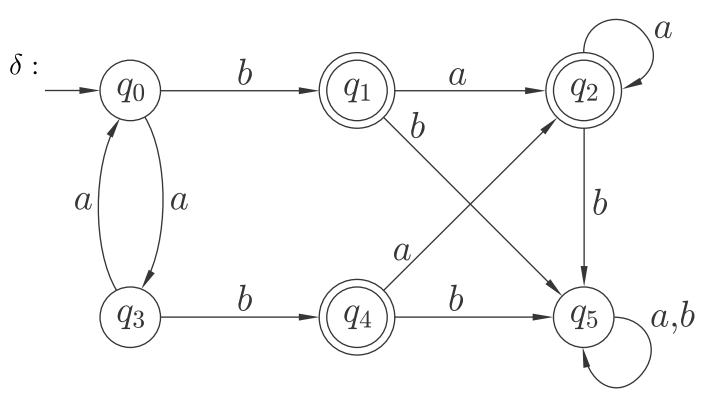
\includegraphics[width=0.8\textwidth]{pics/Blatt9.png}
	\end{center}
\end{figure}

\textbf{Wiederholung:} Approximation $\sim_k$ von $\sim_\A$:
\begin{itemize}
	\item $q\sim_0 q':\Longleftrightarrow (q\in F\Leftrightarrow q'\in F)$
	\item $q\sim_{k+1} q':\Longleftrightarrow(q\sim_k q\wedge\forall a\in\Sigma:\delta(q,a)\sim_k\delta(q',a)$
\end{itemize}
In Aufgabe 8.4 (b) wurde gezeigt:
\begin{align*}
	(\exists k\in\N:\sim_k=\sim_{k+1})\implies\sim_k=\sim_\A
\end{align*}
Bestimme also $\sim_\A$ schrittweise durch Approximation:
\begin{itemize}
	\item $Q|_{\sim_0}=\big\lbrace\lbrace q_1,q_2,q_4\rbrace,\lbrace q_0,q_3,q_5\rbrace\big\rbrace$ Wir trennen also die Endzustände von den Nichtendzuständen (dies ist immer der erste Schritt). Nun ``verfeinern'' wir diese Zerlegung.
	\item $Q|_{\sim_1}=\big\lbrace\lbrace q_1,q_2,q_4\rbrace,\lbrace q_0,q_3,\rbrace,\lbrace q_5\rbrace\big\rbrace$ (``Bleibt $q_i$ in der Äquivalenzklasse?'')
	\item $Q|_{\sim_2}=\big\lbrace\lbrace q_1,q_2,q_4\rbrace,\lbrace q_0,q_3\rbrace,\lbrace q_5\rbrace\big\rbrace=Q|_{\sim_1}\implies \sim_2=\sim_1=\sim_\A$ 
\end{itemize}

Mit $\tilde{q}:=[q|_{\sim_\A}=\lbrace q'\in Q\mid  q\sim_\A g'\rbrace$ erhalten wir:
\begin{align*}
	\tilde{A}&=\big(\lbrace\tilde{q}_1,\tilde{q}_0,\tilde{q}_5\rbrace,\lbrace a,b\rbrace,\tilde{q}_0,\tilde{\delta},
	\underbrace{\lbrace\tilde{q}_1,\tilde{q}_2,\tilde{q}_4\rbrace}_{=\lbrace\tilde{q}_1\rbrace}\big)\mit\\
	\tilde{\delta}(\tilde{q},x)&:=\widetilde{\delta(q,x)}\mit x\in\lbrace a,b\rbrace
\end{align*}

Quotientenautomat $\tilde{\A}$:
\usetikzlibrary{positioning,automata}
\begin{tikzpicture}[shorten >=1pt,node distance=2.7cm,on grid]
  \node[state,initial]   (q_0)                {$\tilde{q}_0$};
  \node[state, accepting](q_1) [right=of q_0] {$\tilde{q}_1$};
  \node[state] (q_5) [right=of q_1] {$\tilde{q}_5$};
  \path[->] (q_0) edge [loop above] node [above] {a} ()
                  edge [bend left=0] node [above] {b} (q_1)
            (q_1) edge [loop above] node [above] {a} ()
            	  edge [bend left=0] node [above] {b} (q_5)
            (q_5) edge [loop above] node [above] {a,b} ();
\end{tikzpicture}

\subsection{Aufgabe 2}
Gegeben sei der DEA
\begin{align*}
	\A=\Big(\lbrace q_0,\ldots,q_8\rbrace,\lbrace a,b\rbrace, q_0,\delta,\lbrace q_3,q_6\rbrace\Big)
\end{align*}
mit
\begin{figure}[H] 
	\begin{center}
		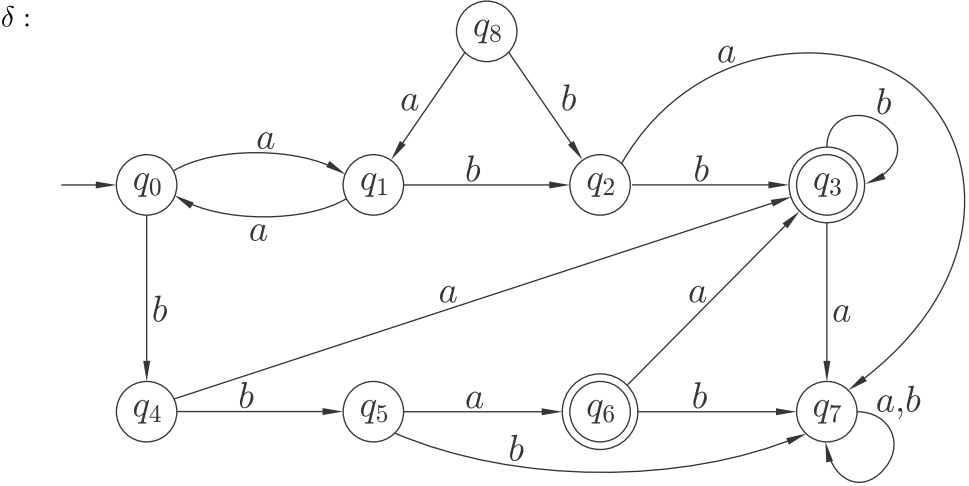
\includegraphics[width=0.8\textwidth]{pics/Blatt9_2.png}
	\end{center}
\end{figure}

Der Vorlesung folgend bezeichne $\A_0$ den zu $\A$ äquivalenten Automaten, den man erhält, indem man alle in $\A$ unerreichbaren Zustände entfernt (und $\delta$ entsprechend anpasst oder einschränkt). 
Hier entspricht $\A_0$ also $\A$ ohne $q_8$.\nl
Nun berechnen wir den Quotientenautomaten $\tilde{\A}_0$ von $\A_0$.\\
Bestimme zuerst $\tilde{\A}_0$: ($Q=\lbrace q_0,\ldots,q_7\rbrace$!)
\begin{itemize}
	\item $Q|_{\sim_0}=\big\lbrace q_3,q_6\rbrace,\lbrace q_0,q_1,q_2,q_4,q_5,q_7\rbrace\big\rbrace$
	\item $Q|_{\sim_1}=\big\lbrace q_3\rbrace,\lbrace q_6\rbrace,\lbrace q_0,q_1,q_7\rbrace,\lbrace q_2\rbrace,\lbrace q_4,q_5\rbrace\big\rbrace$
	% q_5 -> q_3 (in erster Klasse)
	% q_0,q_1 bleiben äquivalent
	\item $Q|_{\sim_2}=\big\lbrace q_3\rbrace,\lbrace q_6\rbrace,\lbrace q_0\rbrace,\lbrace q_1\rbrace,\lbrace q_7\rbrace,\lbrace q_2\rbrace,\lbrace q_4\rbrace,\lbrace q_5\rbrace\big\rbrace$
	\item $Q|_{\sim_3}=Q|_{\sim_2}\implies\sim_3=\sim_2=\sim_{\A_0}$
\end{itemize}
Hier sind also alle Zustände paarweise nicht äquivalent zueinander. 
Der zu $\A$ reduzierte DEA $\A_{\text{red}}$ ist also:
\begin{align*}
	\A_{\text{red}}=\tilde{\A}_0\cong\A_0
\end{align*}
Das heißt, also $\tilde{\A}_0$ isomorph zu $\A_0$ ist (also gleich bis auf Umbenennung der Zustände). Also im Prinzip ist gar nichts passiert (außer, dass $q_8$ entfernt wurde).

\subsection{Aufgabe 3}
Diese Aufgabe zeigt, warum es trotzdem sinnvoll sein kann, Nicht-DEAs zu verwenden.

\subsubsection{Aufgabe 3 a)}
\begin{align*}
	L(\A_n)
	&=\big\lbrace q\in\lbrace a,b\rbrace^\ast\mid\text{der $n$-te Buchstabe von hinten in $w$ ist ein }a\big\rbrace\\
	&=\lbrace a,b\rbrace^\ast\cdot\lbrace a\rbrace\cdot\lbrace a,b\rbrace^{n-1}
\end{align*}

\subsubsection{Aufgabe 3 b)}
$\A_3$:\\
\usetikzlibrary{positioning,automata}
\begin{tikzpicture}[shorten >=1pt,node distance=2.7cm,on grid]
  \node[state,initial]   (q_0)                {$q_0$};
  \node[state](q_1) [right=of q_0] {$q_1$};
  \node[state] (q_2) [right=of q_1] {$q_2$};
  \node[state, accepting] (q_3) [right=of q_2] {$q_3$};
  \path[->] (q_0) edge [loop above] node [above] {a,b} ()
                  edge [bend left=0] node [above] {a} (q_1)
            (q_1) edge [bend left=0] node [above] {a,b} (q_2)
            (q_2) edge [bend left=0] node [above] {a,b} (q_3);
\end{tikzpicture}

Berechnung eines äquivalenten DEA $\A_3'$ durch Potenzmengenkonstruktion:
%TODO tikz-Bild

Umbenennung der Zustände des Quotientenautomaten:
\begin{itemize}
	\item $p_0:=\lbrace q_0\rbrace$
	\item $p_1:=\lbrace q_0,q_1\rbrace$
	\item $p_2:=\lbrace q_0,q_1,q_2\rbrace$
	\item $p_3:=\lbrace q_0,q_2\rbrace$
	\item $p_4:=\lbrace q_0,q_1,q_2,q_3\rbrace$
	\item $p_5:=\lbrace q_0,q_2,q_3\rbrace$
	\item $p_6:=\lbrace q_0,q_1,q_3\rbrace$
	\item $p_7:=\lbrace q_0,q_3\rbrace$
\end{itemize}

Berechnung des Quotientenautomaten (nach Konstruktion gibt es keine unerreichbaren Zustände in obiger Potenzmengenkonstruktion):
\begin{itemize}
	\item $Q|_{\sim_0}=\big\lbrace\lbrace p_4,p_5,p_6,p_7\rbrace,\lbrace p_0,p_1,p_2,p_3\rbrace\big\rbrace$
	\item $Q|_{\sim_1}=\big\lbrace\lbrace p_4,p_5\rbrace,\lbrace p_6,p_7,\lbrace p_0,p_1\rbrace,\lbrace p_2,p_3\rbrace\big\rbrace$
	\item $Q|_{\sim_2}=\big\lbrace\lbrace p_4\rbrace,\lbrace p_5\rbrace,\lbrace p_6\rbrace,\lbrace p_7,\lbrace p_0\rbrace,\lbrace p_1\rbrace,\lbrace p_2\rbrace,\lbrace p_3\rbrace\big\rbrace=Q|_{\sim_3}\implies\sim_2=\sim_3=\sim_{\A'}$
\end{itemize}
Daher gilt: $\A_3\cong(\A_3')_{\text{red}}$ (analog zu Aufgabe 2).

\subsubsection{Aufgabe 3 c)}
Seien also $x=x_1 x_2\hdots x_n\in\lbrace a,b\rbrace^n$ und $y=y_1 y_2\hdots y_n\in\lbrace a,b\rbrace^n$ mit $x\neq y$.\\
Zu zeigen: $x\not\cong_{L(\A_n} y$, d.h.
\begin{align*}
	\exists w\in\lbrace a,b\rbrace^\ast:\big(xw\in L(\A_n)\wedge yw\not\in L(\A_n)\big)\vee\big(xw\not\in L(\A_n)\wedge yw\in L(\A_n)\big)
\end{align*}
Da $x\neq y$, gibt es einen kleinsten Index $j\in\lbrace1,\ldots,n\rbrace$ so, dass $x_j\neq y_j$ (die erste Position von links, an der sich $x$ und $y$ unterscheiden). 
Setze dann 
\begin{align*}
	w:=a^{j-1}
\end{align*}
Dann gibt es zwei Möglichkeiten für $x_j,y_j$:
\begin{enumerate}
	\item $x_j=a$ und $y_j=b$:
	\begin{align*}
		xw&=x_1\hdots x_{j-1}\underbrace{ a x_{j+1}\hdots x_n\underbrace{a\hdots a}_{j-1\text{ viele}}}_{n-(j-1)+(j-1)=n}\in L(\A_n)\\
		yw&=y_1\hdots y_{j-1}\underbrace{ b y_{j+1}\hdots x_n\underbrace{a\hdots a}_{j-1\text{ viele}}}_{n-(j-1)+(j-1)=n}\not\in L(\A_n)
	\end{align*}
	\item $x_j=b$ und $y_j=a$: analog.
\end{enumerate}

Alle paarweise verschiedenen Worte der Länge $n$ über dem Alphabet über $\lbrace a,b\rbrace$ sind nicht äquivalent bzgl. $\cong_{L(\A_n)}$. Da es $2^n$ verschiedene Wörter über $\lbrace a,b\rbrace$ gibt, so gibt es auch mindestens $2^n$ verschiedene Äquivalenzklassen von $\cong_{L(\A_n)}$. Aus Lemma 2.15 (4) folgt damit, dass ein minimaler Automat mindestens $2^n$ Zustände hat.

% This work is licensed under the Creative Commons
% Attribution-NonCommercial-ShareAlike 4.0 International License. To view a copy
% of this license, visit http://creativecommons.org/licenses/by-nc-sa/4.0/ or
% send a letter to Creative Commons, PO Box 1866, Mountain View, CA 94042, USA.

\section{Aufgabenblatt 10}
\subsection*{Aufgabe $\ast$)}
Gegeben ist der $\varepsilon$-NEA
\begin{align*}
	\A=\Big(\lbrace q_0,\ldots,q_4\rbrace,\lbrace a,b\rbrace,q_0,\Delta,\lbrace q_2\rbrace\Big)
\end{align*}

\usetikzlibrary{positioning,automata}
\begin{tikzpicture}[shorten >=1pt,node distance=2.7cm,on grid]
  \node[state,initial]   	(q_0)                		{$q_0$};
  \node[state] 				(q_1) [above right=of q_0] 	{$q_1$};
  \node[state, accepting] 	(q_2) [right=of q_1] 		{$q_2$};
  \node[state] 				(q_3) [below right=of q_0] 	{$q_3$};
  \node[state] 				(q_4) [right=of q_3]		{$q_4$};
  \path[->] (q_0) edge [bend left=0] node [above] {a} (q_1)
                  edge [bend left=0] node [above] {b} (q_3)
            (q_1) edge [bend left=0] node [above] {$\varepsilon$} (q_2)
            	  edge [bend left=0] node [left] {a,b} (q_3)
            (q_2) edge [bend left=0] node [right] {a} (q_3)
                  edge [bend left=0] node [right] {a} (q_4)
            (q_3) edge [bend left=0] node [above] {b} (q_4)
            (q_4) edge [loop right] node [right] {a} ();
\end{tikzpicture}

(Es fällt auf, dass $L(\A)=\lbrace a\rbrace$ ist.)
Zuerst entfernen wir die $\varepsilon$-Transitionen auf naheliegende Weise:

\usetikzlibrary{positioning,automata}
\begin{tikzpicture}[shorten >=1pt,node distance=2.7cm,on grid]
  \node[state,initial]   	(q_0)                		{$q_0$};
  \node[state, accepting]   (q_1) [above right=of q_0] 	{$q_1$};
  \node[state, accepting] 	(q_2) [right=of q_1] 		{$q_2$};
  \node[state] 				(q_3) [below right=of q_0] 	{$q_3$};
  \node[state] 				(q_4) [right=of q_3]		{$q_4$};
  \path[->] (q_0) edge [bend left=0] node [above] {a} (q_1)
                  edge [bend left=0] node [above] {b} (q_3)
            (q_1) edge [bend left=0] node [above] {a} (q_4) %Diese Transition wurde geändert
            	  edge [bend left=0] node [left] {a,b} (q_3)
            (q_2) edge [bend left=0] node [right] {a} (q_3)
                  edge [bend left=0] node [right] {a} (q_4)
            (q_3) edge [bend left=0] node [above] {b} (q_4)
            (q_4) edge [loop right] node [right] {a} ();
\end{tikzpicture}

Wichtig ist hierbei, dass nun $q_1$ auch ein Endzustand geworden ist.
Nun erzeugen wir den äquivalenten DEA mithilfe der Potenzmengenkonstruktion:

\usetikzlibrary{positioning,automata}
\begin{tikzpicture}[shorten >=1pt,node distance=2.7cm,on grid]
  \node[state,initial]   	(q_0)                		{$\lbrace q_0\rbrace$};
  \node[state, accepting]   (q_1) [above right=of q_0] 	{$\lbrace q_1\rbrace$};
  \node[state]			 	(q_3q_4) [right=of q_1] 		{$\lbrace q_3,q_4\rbrace$};
  \node[state] 				(q_3) [below right=of q_0] 	{$\lbrace q_3\rbrace$};
  \node[state]			 	(q_4) [right=of q_3]		{$\lbrace q_4\rbrace$};
  \node[state]				(T)	  [below right =of q_3q_4] {$\emptyset$};
  \path[->] (q_0) edge [bend left=0] node [above] {a} (q_1)
                  edge [bend left=0] node [above] {b} (q_3)
            (q_1) edge [bend left=0] node [above] {a} (q_3q_4)
            	  edge [bend left=0] node [left] {b} (q_3)
            (q_3q_4) edge [bend left=0] node [right] {a,b} (T)
                  %edge [bend left=0] node [right] {a} (q_4)
            (q_3) edge [bend left=0] node [above] {b} (q_4)
            	  edge [bend left=30] node [below] {a} (T)
            (q_4) edge [loop right] node [right] {a} ()
            	  edge [bend left=0] node [below] {b} (T)
           	(T)   edge [loop right] node [above] {a,b} ();
\end{tikzpicture}

Den unerreichbaren Zustand $q_2$ braucht man nicht beachten. Den Papierkorbzustand $\emptyset$ nicht vergessen. Also ist der äquivalente DEA:
\begin{align*}
	\A'&=\Big(\big\lbrace q_0\rbrace,\lbrace q_1\rbrace,\lbrace q_3\rbrace,\lbrace q_3,q_4\rbrace,\lbrace q_4\rbrace,\emptyset\big\rbrace,\lbrace a,b\rbrace,\lbrace q_0\rbrace,\delta,\big\lbrace\lbrace q_1\rbrace\big\rbrace\Big)\\
	\overset{\text{Umbennung}}&{=:}
	\Big(\underbrace{\lbrace p_0, p_1,p_3,p_2,p_4, p_5\rbrace}_{=:P},\lbrace a,b\rbrace,p_0,\delta,\lbrace p_1\rbrace\Big)
\end{align*}

Da $\A'$ keine unerreichbaren Zustände mehr besitzt, gilt $\A_0=\A'$.
Um $\A_{\text{red}}$ zu berechnen, berechnen wir $\sim_{\A}$ schrittweise durch $\sim_k$:
\begin{itemize}
	\item $P|_{\sim_0}=\big\lbrace\lbrace p_1\rbrace,\lbrace p_0,p_2,p_3,p_4,p_5\rbrace\big\rbrace$ (Startzustände und Endzustände trennen)
	\item $P|_{\sim_1}=\big\lbrace\lbrace p_1\rbrace,\lbrace p_0\rbrace,\lbrace p_2,p_3,p_4,p_5\rbrace\big\rbrace$
	\item $P|_{\sim_2}=\big\lbrace\lbrace p_1\rbrace,\lbrace p_0\rbrace,\lbrace p_2,p_3,p_4,p_5\rbrace\big\rbrace$
\end{itemize}
Es gilt also $\sim_2=\sim_1\implies\sim_\A=\sim_1$. 
Der Quotientenautomat
\begin{align*}
	\tilde{A}&=\big(\tilde{Q},\Sigma,\tilde{q}_0,\tilde{\delta},\tilde{F}\big)\mit\\
	\tilde{Q}&=\big\lbrace\lbrace p_1\rbrace,\lbrace p_0\rbrace,\lbrace p_2,p_3,p_4,p_5\rbrace\big\rbrace
	=
	\big\lbrace [p_1]_{\sim},[p_0]_\sim,[p_2]_\sim\big\rbrace\\
	\Sigma&=\lbrace a,b\rbrace\\
	\tilde{q}_0&=\lbrace p_0\rbrace=[p_0]_\sim\\
	\tilde{\delta}&=\left\lbrace
		\begin{array}{l}
			\big([p_0]_{\sim},a,[p_1]_{\sim}\big), \big([p_0]_{\sim},b,[p_2]_{\sim}\big),\\
			\big([p_1]_{\sim},a,[p_2]_{\sim}\big), \big([p_1]_{\sim},b,[p_2]_{\sim}\big),\\
			\big([p_2]_{\sim},a,[p_2]_{\sim}\big), \big([p_2]_{\sim},b,[p_2]_{\sim}\big)
		\end{array}
	\right\rbrace\\
	\tilde{F}&=\big\lbrace \lbrace p_1\rbrace\big\rbrace=\big\lbrace [p_1]_\sim\big\rbrace
\end{align*}
erfüllt also
\begin{align*}
	\A_{\text{red}}=\tilde{\A_0}\cong\A_0=\A'
\end{align*}
und insbesondere gilt
\begin{align*}
	L\big(\A_\red\big)=\lbrace a\rbrace.
\end{align*}

\begin{tikzpicture}[shorten >=1pt,node distance=2.7cm,on grid]
  \node[state,initial]   	(q_0)                		{$[p_0]_{\sim}$};
  \node[state, accepting]   (q_1) [above right=of q_0] 	{$[p_1]_{\sim}$};
  \node[state] 				(q_2) [below right=of q_0] 	{$[p_2]_{\sim}$};
  \path[->] (q_0) edge [bend left=0] node [above] {a} (q_1)
                  edge [bend left=0] node [above] {b} (q_2)
            (q_1) edge [bend left=0] node [right] {a,b} (q_2)
            (q_2) edge [loop right]  node [above] {a,b} ();
\end{tikzpicture}

\subsection{Aufgabe 1}
\textbf{Konvention.} Bei mir ist $\N:=\lbrace 1,2,3,\ldots\rbrace$.\nl
Meine Idee (geht sicher viel eleganter):\\
Da es sehr viele Zerlegungsmöglichkeiten pro Wort $w$ gibt, ist es geschickter zu schauen, für welche $y\in\Sigma^+$ überhaupt die Eigenschaft 
\begin{align*}
	\exists x,z\in\Sigma^\ast:\forall k\in\N:xy^kz\in L(\A)
\end{align*}
gilt.
Man sieht, dass nur $y\in\lbrace c,cd,dc\rbrace=:M$ dies erfüllen. Nun gehen wir $w$ einzeln durch und schauen uns nur die Zerlegungen an, bei der $y\in M$ gilt (denn nur die sind interessant). Da $x,z=\varepsilon$ möglich, erhalten wir genau diese möglichen Zerlegungen durch \textit{Stringvergleich}, d.h. wir schauen, ob ein $p\in M$ existiert, welches ein Substring von dem festen $w$ ist. Also: (Nutze Kurzschreibweise $\alpha|\beta|\gamma$ für Zerlegung des Wortes $w$ in $x=\alpha$, $y=\beta$ und $z=\gamma$)
\begin{itemize}
	\item $w=adc$: Mögliche Zerlegungen: 
	\begin{itemize}
		\item $ad|c|\varepsilon$: ist in $L(\A)$, aber $c$ dann nicht mehr loopbar.
		\item $a|dc|\varepsilon$: ist in $L(\A)$ und erfüllt \eqref{eqAufgabe1}.
	\end{itemize}
	\item $w=cda$ ist gar nicht in $L(\A)$, weshalb keine solche Zerlegungen existieren können, die \eqref{eqAufgabe1} erfüllen. 
	\item $w=bcdc$ Mögliche Zerlegungen: 
	\begin{itemize}
		\item $b|c|dc$: erfüllt \eqref{eqAufgabe1}.
		\item $bcd|c|\varepsilon$: erfüllt \eqref{eqAufgabe1} nicht, da $c$ nicht mehr "geloopt" werden kann, nach $acd$ gelesen wurde.
		\item $b|cd|c$: erfüllt \eqref{eqAufgabe1}.
		\item $bc|dc|\varepsilon$: erfüllt \eqref{eqAufgabe1}.
	\end{itemize}
	\item $w=acdc$ Mögliche Zerlegungen: 
	\begin{itemize}
		\item $a|c|dc$: erfüllt \eqref{eqAufgabe1}.
		\item $acd|c|\varepsilon$ erfüllt \eqref{eqAufgabe1} nicht, da $c$ dann nicht mehr geloopt werden kann.
		\item $ac|dc|\varepsilon$ erfüllt \eqref{eqAufgabe1}.
		\item $a|cd|c$ erfüllt \eqref{eqAufgabe1}.
	\end{itemize}
\end{itemize}
Somit erhalten wir für $adc$ 1, für $cda$ 0, für $bcdc$ 3 und für $acdc$ 3 Zerlegungen, die die gesuchten Eigenschaft erfüllen:

\begin{align}\label{eqAufgabe1}
	\forall k\in\N:xy^kz\in L(\A)
\end{align}

\textbf{Tutor-Lösung: (stimmt mit meiner überein)}
\begin{itemize}
	\item $w=adc\in L(\A)$: kein Zerlegung möglich bei der $y$ auch wegfallen kann
	\item $w=cda\not\in L(\A)$: keine "pumpbare" Zerlegung möglich, da nicht in der Sprache
	\item $w=bcdc\in L(\A)$:
	\begin{itemize}
		\item $x=b,\qquad,y=c,\qquad z=dc$
		\item $x=b,\qquad y=cd,\qquad z=c$
		\item $x=bc,\qquad y=dc,\qquad z=\varepsilon$
	\end{itemize}
	\item $w=acdc\in L(\A)$:
	\begin{itemize}
		\item $x=a,\qquad y=c,\qquad z=dc$
		\item $x=ac,\qquad y=dc,\qquad z=\varepsilon$
		\item $x=a,\qquad y=cd,\qquad z=\varepsilon$ 
	\end{itemize}
\end{itemize}

Beachte: falls man $0\in\N$ annimmt, entfallen noch einige Fälle oben.

\subsection{Aufgabe 2}
Die Sprache
\begin{align*}
	L:=\big\lbrace a^p\mid p\text{ ist Primzahl}\big\rbrace\mit\Sigma:=\lbrace a\rbrace
\end{align*}
ist nicht erkennbar.

\begin{proof}
	Wir führen einen Widerspruchsbeweis: Angenommen, $L$ ist erkennbar.
	Dann folgt aus dem Pumping-Lemma (3.1): Es gibt $n_0\in\N_{\geq1}$ so, dass jedes Wort $w\in L$ mit $|w|\geq n_0$ sich zerlegen lässt in $w=xyz$ mit $y\neq\varepsilon$ und $xy^kz\in L$ für alle $k\geq0$.
	Sei also $w=a\ldots a\in L$ beliebig mit $p\geq n_0$. Also gilt
	\begin{align*}
		&w=\underbrace{a\ldots a}_{p\geq n_0\text{ Stück}}\overset{!}= xy^k z\\
		&\implies \exists l,m,n\in\N_{\geq0}: w=a^p=a^l a^m a^n\\
		&\implies p=l+m+n
	\end{align*}
	Nach Voraussetzung ist $p$ eine Primzahl und nach Pumpinglemma gilt:
	\begin{align*}
		&x y^k z\in L &\forall k\in\N_{\geq0}\\
		&\implies l+m\cdot k+ n\text{ ist Primzahl} &\forall k\in\N_{\geq0}
	\end{align*}
	Dies ist aber im Allgemeinen keine Primzahl (was ich gerade leider nicht für alle Fälle zeigen kann...).\\
	Widerspruch! Somit ist $L$ nicht erkennbar.
\end{proof}

\begin{proof}[Beweis des Tutors.]\enter
	\textbf{Pumping-Lemma (vereinfacht)}:\\
	Für jede erkennbare Sprache $L$ existiert ein $n_0\in\N$ so, dass\\
	für alle Wörter $w\in L$ mit $|w|\geq n_0$\\
	existiert eine Zerlegung $w=xyz$ mit $y\neq\varepsilon$ so, dass\\
	für alle $k\in\N$ gilt: $xy^kz\in L$.\nl
	Beweis durch Widerspruch:
	Angenommen, $L$ wäre erkennbar. Dann gilt das Pumpinglemma (vereinfacht) auch für $L$.
	Sei $p$ ein Primzahl mit $p\geq n_0$ (existiert nach Satz von Euklid: Es gibt unendlich viele Primzahlen).
	Dann gilt:
	$a^p\in L$ und $|a^p|\geq n_0$.
	Damit muss es eine Zerlegung von $a^p=xyz$ geben $\rightsquigarrow x=a^n,y=a^m,z=a^{n_2}$ mit $n_1,n_2,m\in\N$ und $m>0$.
	Also gilt $p=n_1+n_2+m$. 
	Definiere $n:=n_1+n_2$.
	Da $a^p=a^{m+n}\in L$, folgt aus dem Pumping-Lemma,
	dass auch $a^{n+k\cdot m}\in L$ für alle $k\in\N$.
	Insbesondere für $k=n$ %Die Idee, die mir fehlte!
	gilt $a^{n+n\cdot m}\in L$.
	Aber falls $n\neq1$ (also $n>1$ oder $n=0$) ist $n+n\cdot m=n\cdot(m+1)$ keine Primzahl!\\
	Falls $n=1$, dann müsste $a^{n+0\cdot m}=a^n=a\in L$ gelten. Widerspruch!
\end{proof}

\subsection{Aufgabe 3}
Die Sprache
\begin{align*}
	L:=\Big\lbrace w\mid w=1^k\text{ für }k\geq0\text{ oder }w=0^j1^p\text{ für }j\geq1\text{ und }p\text{ Primzahl}\Big\rbrace\\
	\mit\Sigma=\lbrace0,1\rbrace
\end{align*}
ist nicht erkennbar.

\begin{proof}
	\textbf{Pumping-Lemma (verschärft, Änderungen unterstrichen)}:\\
	Für jede erkennbare Sprache $L$ existiert ein $n_0\in\N$ so, dass\\
	%für alle Wörter $w\in L$ mit $|w|\geq n_0$ 
	\underline{für alle Wörter $u,v,w$ mit $uvw\in L$ und $|w|\geq n_0$}\\
	existiert eine Zerlegung $\underline{v}=xyz$ mit $y\neq\varepsilon$ so, dass\\
	für alle $k\in\N$ gilt: $xy^kz\in L$.\nl
	Das vereinfachte Pumpinglemma kann hier zwar auch wieder angewendet werden, hilft uns aber nicht, da
	alle $w\in L$ mit $|w|>0$ "pumpbar" zerlegt werden können:
	\begin{itemize}
		\item $w=1^k\rightsquigarrow x=1^{k-1},y=1,z\varepsilon$
		\item $w=0^j 1^p\rightsquigarrow x=\varepsilon,y=0^j,z=1^p$
	\end{itemize}
	Es gibt also eine gültige Zerlegung, weshalb wir mit dem vereinfachten Pumpinglemma keinen Widerspruch herleiten können.
	Mit dem Pumping-Lemma in verschärfter Form kann das Ergebnis aus Aufgabe 10.2 genutzt werden:
	Sei $p$ eine Primzahl mit $p\geq n_0$. Zerlege dann das Wort $01^p$ in $u=0$, $v=1^p$ und $w=\varepsilon$.
	Es gilt $01^p\in L$ und $|v|\geq n_0$.
	Zerlege dann $v$ nun wie in 10.2 gezeigt.
\end{proof}

\subsection{Aufgabe 4}
\textbf{Satz 4.1} Ist $L$ erkennbar, so ist auch $L^\ast$ erkennbar.

\begin{proof}
	%Erinnerung: Eine Sprache $L$ ist per Definition erkennbar, wenn es einen NEA $\A$ gibt, der $L$ akzeptiert, d.a. $L=L(\A)$.\nl
	Da $L$ erkennbar ist, gibt es per Definition einen NEA
	\begin{align*}
		\A:=(Q,\Sigma,q_0,\Delta,F)
	\end{align*}
	mit $L(\A)=L$. 
	Sei nun $q_{0\varepsilon}\not\in Q$ und setze
	\begin{align*}
		\A_\varepsilon&:=\Big(Q\cup\lbrace q_{0\varepsilon}\rbrace,\Sigma,q_{0\varepsilon},\Delta_\varepsilon,\lbrace q_{0\varepsilon}\rbrace\Big)\\
		\Delta_\varepsilon&:=\Delta\cup\underbrace{\big\lbrace(f,\varepsilon,q_{0\varepsilon}):f\in F\big\rbrace}_{
			=\big(F\times\lbrace\varepsilon\rbrace\times\lbrace q_{0\varepsilon}\rbrace\big)
		}\cup\big\lbrace(q_{0\varepsilon},\varepsilon,q_{0})\big\rbrace\Big)
	\end{align*}
	
	
  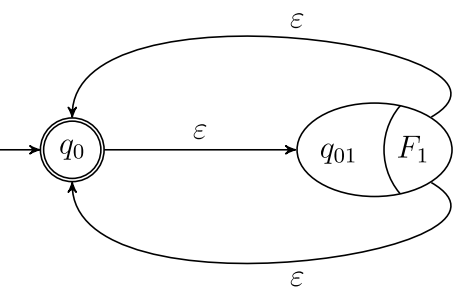
\includegraphics[width=0.7\textwidth]{pics/Blatt10_4.png}
  
  Offenbar ist $\A_\varepsilon$ ein $\varepsilon$-NEA. Mit Lemma 1.12 bekommt man einen zu $\A_\varepsilon$ äquivalenten NEA, nennen wir ihn $\A_{\text{NEA}}$. Äquivalent bedeutet $L(\A_\varepsilon)=L(\A_{\text{NEA}})$.\nl
  Bleibt noch zu zeigen, dass $L(\A_\varepsilon)=L^\ast$ gilt. 
  Sei also $w\in L^\ast$.
  Dann gibt es ein $n\in\N$ so, dass $w\in\bigcup\limits_{i=0}^n L$ ist. Man sieht leicht, dass $w\in L(\A_\varepsilon)$ liegen muss. (Das formal aufzuschreiben ist ein wenig sperrig.)
\end{proof}

\subsection{Aufgabe 5}
Folgende Automatenklassen sind in ihrer Ausdrucksstärke gleichmächtig zueinander:
NEA, $\varepsilon$-NEA (entfernen von $\varepsilon$-Transitionen), NEA mit Wortübergängen (Zwischenzustände einführen), DEA (Potenzmengenkonstruktion)\\
Transitionssysteme sind \underline{nicht} äquivalent zu obigen.\nl
Beweise oder Widerlege:
\begin{enumerate}[label=\alph*)]
	\item $L$ erkennbar $\implies\exists\varepsilon$-NEA $\A:L(\A)=L$.\\
	Stimmt, denn:
	\begin{align*}
		L\text{ erkennbar}
		\overset{\text{Def 1.6}}&\Longleftrightarrow
		\exists\text{NEA}\A_N:L(\A_N)=L\\
		\overset{\text{Lemma 10}}&\Longleftrightarrow
		\exists\varepsilon\text{-NEA }\A:L(\A)\overset{\text{Def 1.6}}{=}L(\A_N)=L
	\end{align*}
	\item $\exists$ NEA mit Wortübergängen mit $L(\A)=L\implies L$ erkennbar.\\
	Stimmt, denn:
	\begin{align*}
		&\exists\text{ NEA $\A$ mit Wortübergängen mit }L(\A)=L\\
		\overset{\text{Satz 1.9}}&\implies
		\exists\text{ NEA }\A_N:L(\A_N)\overset{\text{Def 1.6}}=L(\A)=L\\
		\overset{\text{Def 1.6}}&\implies
		L\text{ erkennbar}
	\end{align*}
	\item $\exists$ Transitionssystem $\A$ mit $L(\A)=L\implies L$ erkennbar\\
	Das stimmt nicht, Gegenbeispiel:
	\begin{align*}
		L:=\Big\lbrace a^p:p\text{ ist Primzahl }\Big\rbrace
	\end{align*}
	Transitionssystem: (wird endliche Kette, Endzustände sind Primzahlen)
	\item $L$ erkennbar und $L\subseteq L'\implies L'$ erkennbar\\
	Stimmt nicht, Gegenbeispiel:
	\begin{align*}
		L:=\lbrace aa\rbrace\qquad
		L':=\Big\lbrace a^p:p\text{ ist Primzahl }\Big\rbrace
	\end{align*}
	\item $L$ erkennbar und $L'\subseteq L\implies L'$ erkennbar.\\
	Stimmt nicht, Gegenbeispiele:
	\begin{align*}
		&L=\Big\lbrace a^n:n\in\N\big\rbrace,& l'=\big\lbrace a^p:p\text{ ist Primzahl }\Big\rbrace\\
		&L_2=\Sigma^\ast, &\Big\lbrace a^n b^n:n\in\N\Big\rbrace
	\end{align*}
	\item $L_1,L_2$ erkennbar $\implies L:=L_1\cap L_2$ erkennbar.\\
	Stimmt, wegen Satz 4.1.
	\item Wenn es ein $n\in\N$ gibt, so dass $\cong_L$ (Nerode-Rechtskongruenz) höchstens $n$ Äquivalenzklassen hat, so ist $L$ erkennbar.\\
	Ja, dies ist eine Richtung des Satzes von Myhill-Nerode
	($L$ ist erkennbar / regulär $\Longleftrightarrow \, \cong_L$ hat endlichen Index / endliche viele Äquivalenzklassen)
\end{enumerate}


% This work is licensed under the Creative Commons
% Attribution-NonCommercial-ShareAlike 4.0 International License. To view a copy
% of this license, visit http://creativecommons.org/licenses/by-nc-sa/4.0/ or
% send a letter to Creative Commons, PO Box 1866, Mountain View, CA 94042, USA.

\section{Aufgabenblatt 11}
\subsection*{Aufgabe $\ast$)}
%TODO

\subsection*{Aufgabe $\ast\ast$)}
%TODO

\subsection{Aufgabe 1}
Seien $r,s$ reguläre Ausdrücke, Beachte $r=s:\Longleftrightarrow L(r)=L(s)$ (eigentlich $r\equiv s$). Dann gilt:
\begin{enumerate}[label=\alph*)]
	\item $r+s=s+r$
	\item $(r+s)+t=r+(s+t)$
	\item $(rs)t=r(st)$
	\item $r(s+t)=rs+rt$
	\item $\emptyset^\ast=\varepsilon$
	\item $(r^\ast)^\ast=r^\ast$
	\item $r^\ast=rr^\ast+\varepsilon$
	\item $(\varepsilon+r)^\ast=r^\ast$
\end{enumerate}

\begin{proof}
	\underline{Zeige a):}
	\begin{align*}
		r+s
		\overset{\text{Not}}&=		
		L(r+s)
		\overset{\text{Def}}=
		L(r)\cup L(s)
		\overset{\text{Kommu. von }\cup}=
		L(s)\cup L(r)
		\overset{\text{Def}}=
		L(s+r)
		\overset{\text{Not}}=	
		s+r
	\end{align*}
	\underline{Zeige b):}
	\begin{align*}
		L\big((r+s)+t\big)
		\overset{\text{}}&=
		L(r+s)\cup L(t)\\
		\overset{\text{}}&=
		\big(L(r)\cup L(s)\big)\cup L(t)\\
		\overset{\text{Asso. von }\cup}&=
		L(r)\cup\big(L(s)\cup L(t)\big)\\
		\overset{\text{}}&=
		L(r)\cup L(s+t)\\
		\overset{\text{}}&=
		L\big(r+(s+t)\big)
	\end{align*}
	
	\underline{Zeige c):} "Ersetze Punkt durch Konkatenationsoperator auf Sprachen":
	\begin{align*}
		L\big((r\cdot s)\cdot t\big)
		\overset{\text{}}&=
		L(r\cdot s)\cdot L(t)\\
		\overset{\text{}}&=
		\big(L(r)\cdot L(s)\big)\cdot L(t)\\
		\overset{\text{}}&=
		\big\lbrace ab:a\in L(r)\cdot L(s)\wedge b\in L(t)\big\rbrace\\
		\overset{\text{}}&=
		\Big\lbrace ab:a\in\big\lbrace cd:c\in L(r)\wedge d\in L(s)\big\rbrace\wedge b\in L(t)\Big\rbrace\\
		\overset{\text{}}&=
		\Big\lbrace cdb:\big(c\in L(r)\wedge d\in L(s)\big)\wedge b\in L(t)\Big\rbrace\\
		\overset{\text{Asso. von }\wedge}&=
		\Big\lbrace cdb:c\in L(r)\wedge\big(d\in L(s)\wedge b\in L(t)\big)\Big\rbrace\\
		\overset{\text{}}&=
		\Big\lbrace ce:c\in L(r)\wedge e\in\big\lbrace db:d\in L(s)\wedge b\in L(t)\big\rbrace\Big\rbrace\\
		\overset{\text{}}&=
		\big\lbrace ce:c\in L(r)\wedge e\in L(s)\cdot L(t)\big\rbrace\\
		\overset{\text{}}&=
		L(r)\cdot\big(L(s)\cdot L(t)\big)\\
		\overset{\text{}}&=
		L(r)\cdot L(s\cdot t)\\
		\overset{\text{}}&=
		L\big(r\cdot(s\cdot t)\big)
	\end{align*}
	
	\underline{Zeige d):}
	\begin{align*}
		L\big(r(s+r)\big)
		\overset{\text{Def}}&=
		L(r)\cdot L(s+t)\\
		\overset{\text{}}&=
		L(r)\cdot\big(L(s)\cup L(t)\big)\\
		\overset{\text{Aufgabe 7.2 (a)}}&=
		L(r)\cdot L(s)\cup L(r)\cdot L(t)\\
		\overset{\text{}}&=
		L(r\cdot s)\cup L(r\cdot t)\\
		\overset{\text{}}&=
		L(rs+rt)
	\end{align*}		
	
	\underline{Zeige e):}
	Achtung! Hier ist \underline{nicht} der Kleene-Stern gemeint. 
	Er ist definiert als der Kleene-Stern der Sprache,
	\begin{align*}
		L(\underbrace{\emptyset^\ast}_{\text{Regex}})
		\overset{\text{}}&=
		L(\underbrace{\emptyset}_{\text{Regex}})^\ast
		\overset{\text{}}=
		\underbrace{\emptyset}_{\text{Sprache}}^\ast
		\overset{\text{Def }\ast}=
		\bigcup\limits_{n=0}^\infty
		\overset{\text{}}=
		\varepsilon\cup\emptyset\cup\ldots
		\overset{\text{}}=
		\lbrace\underbrace{\varepsilon}_{\text{leeres W}}\rbrace
		\overset{\text{}}=
		L(\underbrace{\varepsilon}_{\text{Regex}})
	\end{align*}
	
	\underline{Zeige f):}
	\begin{align*}
		L\big((r^\ast)^\ast\big)
		\overset{\text{}}&=
		L(r^\ast)^\ast
		\overset{\text{}}=
		\big(L(r)^\ast\big)^\ast
		\overset{\text{Aufg 7.2 (d)}}=
		L(r)^\ast
		\overset{\text{}}=
		L(r^\ast)
	\end{align*}
	Beachte: Alle $\ast$-Symbole innerhalb $L(\ldots)$ bezeichnen den Sternoperator der regulären Ausdrücke.
	Alle $\ast$-Symbole außerhalb $L(\ldots)$ bezeichnet den Kleene-Stern.
	
	\underline{Zeige g):}
	\begin{align*}
		L(r^\ast)
		\overset{\text{}}&=
		L(r)^\ast\\
		\overset{\text{}}&=
		\bigcup\limits_{n=0}^\infty L(r)^n\\
		\overset{\text{}}&=
		L(r)^0\cup\bigcup\limits_{n=1}^\infty L(r)^n\\
		\overset{\text{}}&=
		L(r)^0\cup L(r)\cdot\left(\bigcup\limits_{n=0}^\infty L(r)^n\right)\\
		\overset{\text{}}&=
		\lbrace\varepsilon\rbrace\cup L(r)\cdot L(r)^\ast\\
		\overset{\text{}}&=
		L(\varepsilon)\cup L(r)\cdot L(r^\ast)\\
		\overset{\text{}}&=
		L(\varepsilon)\cup L(r\cdot r^\ast)\\
		\overset{\text{}}&=
		L(\varepsilon+rr^\ast)\\
		\overset{\text{a)}}&=
		L(rr^\ast+\varepsilon)
	\end{align*}
	
	\underline{Zeige h):}
	\begin{align*}
		L\big((\varepsilon+r)^\ast\big)
		\overset{\text{}}&=
		L(\varepsilon+r)^\ast\\
		\overset{\text{}}&=
		\big(L(\varepsilon)\cup L(r)\big)^\ast\\
		\overset{\text{}}&=
		\big(\lbrace\varepsilon\rbrace\cup L(r)\big)^\ast\\
		\overset{\text{}}&=
		L(r)^\ast\\
		\overset{\text{}}&=
		L(r^\ast)
	\end{align*}
\end{proof}

\subsection{Aufgabe 2}
Verwenden Sie die Konstruktion aus dem Beweis von Satz von Kleene (Satz 5.4) und das
Lemma von Arden (Lemma 5.6), um einen regulären Ausdruck $r$ anzugeben, der die von dem
folgenden Automaten $\A$ akzeptierte Sprache repräsentiert (das heißt, es soll $L(r) = L(\A)$ gelten).

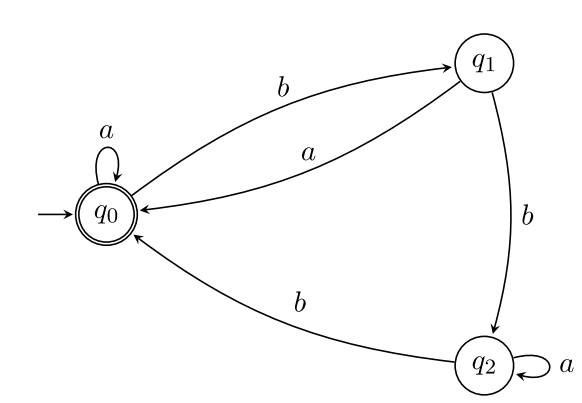
\includegraphics[width=0.7\textwidth]{pics/Blatt11_2.png}
 
\begin{lösung}
	\textbf{Lemma von Arden:}
	Seien $A,B\subseteq\Sigma^\ast$ und $\varepsilon\not\in A$.
	Dann hat
	\begin{align}\label{eqLemmaArden}\tag{Arden}
		X=A\cdot X\cup B
	\end{align}
	die eindeutige Lösung $X=A^\ast\cdot B$.\nl
	Wir erzeugen nun für jeden Zustand $q\in Q$ eine Gleichung.
	\begin{align}\label{eq2_1}
		X_0&=\lbrace a\rbrace\cdot X_0\cup\lbrace b\rbrace\cdot X_1\cup\lbrace\varepsilon\rbrace\\\label{eq2_2}
		X_1&=\lbrace a\rbrace\cdot X_0\cup\lbrace b\rbrace\cdot X_2\\
		X_2&=\lbrace a\rbrace\cdot X_2\cup\lbrace b\rbrace\cdot X_0\label{eq2_3}
	\end{align}
	Notizen:
	\begin{itemize}
		\item Bei Endzuständen muss $\cup\lbrace\varepsilon\rbrace$ ergänzt werden.
		\item Man schaut sich alle ausgehenden Transitionen an.
	\end{itemize}
	Wende nun Lemma von Arden auf \eqref{eq2_3} an:
	\begin{align}\label{eq2_4}
		X_2&=\lbrace a\rbrace^\ast\cdot\lbrace b\rbrace\cdot X_0 &\text{Lemma auf \eqref{eq2_3}}\\\nonumber
		X_1&=\lbrace a\rbrace\cdot X_0\cup\lbrace b\rbrace\cdot\lbrace a\rbrace^\ast\cdot\lbrace b\rbrace\cdot X_0 &\text{Einsetzen von \eqref{eq2_4} in \eqref{eq2_2}}\\
		&=\Big(\lbrace a\rbrace\cup\lbrace b\rbrace\cdot\lbrace a\rbrace^\ast\cdot\lbrace b\rbrace\Big)\cdot X_0\label{eq2_5}\\
		X_0&=\lbrace a\rbrace\cdot X_0\cup\lbrace b\rbrace\Big(\lbrace a\rbrace\cup\lbrace b\rbrace\cdot\lbrace a\rbrace^\ast\cdot\lbrace b\rbrace\Big)\cdot X_0\cup\lbrace\varepsilon\rbrace &\text{Einsetzen von \eqref{eq2_5} in \eqref{eq2_1}}\nonumber\\
		\overset{\text{Distr}}&{=}
		\Big(\lbrace a\rbrace\cup\lbrace b\rbrace\cdot\big(\lbrace a\rbrace\cup\lbrace b\rbrace\cdot\lbrace a\rbrace^\ast\cdot\lbrace b\rbrace\big)\Big)\cdot X_0\cup\lbrace\varepsilon\rbrace\label{eq2_6}\\
		X_0&=\Big(\lbrace a\rbrace\cup\lbrace b\rbrace\cdot\big(\lbrace a\rbrace\cup\lbrace b\rbrace\cdot\lbrace a\rbrace^\ast\cdot\lbrace b\rbrace\big)\Big)^\ast\cdot\lbrace\varepsilon\rbrace &\text{Lemma auf \eqref{eq2_6}}\nonumber\\
		&=L\Big(\big(a+b\cdot(a+ba^\ast b)\big)^\ast\Big)\nonumber\\
		&=L\Big(\big(a+ba+bba^\ast b\big)^\ast\Big)\nonumber
	\end{align}
\end{lösung} 

\subsection{Aufgabe 3}
Sei $\Sigma=\lbrace a,b,c\rbrace$.
 Geben Sie für jede der folgenden Sprachen $L_i$ einen regulären Ausdruck $r_i$ mit $L_i=L(r)$ an.
Erklären Sie die Wahl Ihrer regulären Ausdrücke $r_i$.

\begin{enumerate}[label=\alph*)]
	\item $L_1=\big\lbrace w\in\Sigma^\ast:w\text{ beginnt mit $a$ mit $|w|_b$ ist gerade}\big\rbrace$
	\item $L_2=\big\lbrace w\in\Sigma^\ast:\nexists u,v\in\Sigma^\ast:w=uaav\big\rbrace$
\end{enumerate}

\begin{lösung}
	Idee: 
	\begin{enumerate}
		\item Konstruiere NEA $\A_i$ mit $L(\A_i)=L_i$.
		\item Ermittle den regulären Ausdruck $r_i$ von $\A_i$ wie in Aufgabe 2.
	\end{enumerate}		

	\underline{Zeige a):}
	
	\usetikzlibrary{positioning,automata}
\begin{tikzpicture}[shorten >=1pt,node distance=2.7cm,on grid]
  \node[state,initial]   	(q_0)                		{$q_0$};
  \node[state, accepting] 	(q_1) [above right=of q_0] 	{$q_1$};
  \node[state] 	(q_2) [below=of q_1] 		{$q_2$};
  \path[->] (q_0) edge [bend left=0] node [above] {a} (q_1)
            (q_1) edge [loop right] node [above] {a,c} ()
            	  edge [bend left=30] node [left] {b} (q_2)
            (q_2) edge [loop right] node [right] {a,c} ()
                  edge [bend left=30] node [right] {b} (q_1)
       ;
\end{tikzpicture}

	$q_1\hat{=}$ "gerade Anzahl von b's gelesen"\\
	$q_2\hat{=}$ "ungerade Anzahl von b's gelesen"
	
	\begin{align}
		X_0&=\lbrace a\rbrace\cdot X_1\\
		X_1&=\lbrace a,c\rbrace\cdot X_1\cup\lbrace b\rbrace\cdot X_2\cup\lbrace\varepsilon\rbrace\\
		X_2&=\lbrace a,c\rbrace\cdot X_2\cup\lbrace b\rbrace\cdot X_1
	\end{align}
	
	Mit dem Lemma von Arden erhalten wir (anwenden auf letzte Gleichung):
	\begin{align*}
		X_2&=\lbrace a,c\rbrace^\ast\cdot\lbrace b\rbrace\cdot X_1\\
		X_1&=\lbrace a,c\rbrace\cdot X_1\cup\lbrace b\rbrace\cdot\lbrace a,c\rbrace^\ast\cdot\lbrace b\rbrace\cdot X_1\cup\lbrace\varepsilon\rbrace\\
		&=\Big(\lbrace a,c\rbrace\cup\lbrace b\rbrace\cdot\lbrace a,c\rbrace^\ast\cdot\lbrace b\rbrace\Big)\cdot X_1 \cup\lbrace\varepsilon\rbrace\\
		X_1&=\Big(\lbrace a,c\rbrace\cup\lbrace b\rbrace\cdot\lbrace a,c\rbrace^\ast\cdot\lbrace b\rbrace\Big)^\ast\cdot\lbrace\varepsilon\rbrace\\
		X_0&=\lbrace a\rbrace\cdot\Big(\lbrace a,c\rbrace\cup\lbrace b\rbrace\cdot\lbrace a,c\rbrace^\ast\cdot\lbrace b\rbrace\Big)^\ast\\
		&=L\Big(a\cdot\big((a+c)+b(a+c)^\ast b\big)^\ast\Big)=:r_i
	\end{align*}		
	
	\underline{Zeige b):}
	Sprache umschreiben:
	\begin{align*}
		L_2&=\big\lbrace w\in\Sigma^\ast:\nexists u,v\in\Sigma^\ast:w=uaav\big\rbrace\\
		&=\big\lbrace w\in\Sigma^\ast: w\text{ enthält keine zwei aufeinanderfolgenden $a$'s}\big\rbrace
	\end{align*}
	
	\begin{tikzpicture}[shorten >=1pt,node distance=2.7cm,on grid]
  \node[state,initial, accepting](q_0)           		{$q_0$};
  \node[state, accepting] 	(q_1) [right=of q_0] 	{$q_1$};
  \path[->] (q_0) edge [loop above] node [above] {b,c} ()
  				  edge [bend left=30] node [above] {a} (q_1)
            (q_1) edge [bend left=30] node [below] {b,c} (q_0)
       ;
	\end{tikzpicture}

	\begin{align*}
		r_1=\big(b+c+a\cdot(b+c)\big)^\ast\cdot(a+\varepsilon)
	\end{align*}
	
	
\end{lösung}


% This work is licensed under the Creative Commons
% Attribution-NonCommercial-ShareAlike 4.0 International License. To view a copy
% of this license, visit http://creativecommons.org/licenses/by-nc-sa/4.0/ or
% send a letter to Creative Commons, PO Box 1866, Mountain View, CA 94042, USA.

\section{Aufgabenblatt 12}
\subsection*{Aufgabe $\ast$)}
Die dritte Bedingung in $L$ sagt, dass die Wörter in $L$ nicht mit $a$ beginnen dürfen.
Kurz geschrieben (Achtung, keine offizielle Notation!)
\begin{align*}
	L=\Big\lbrace w=u_1 babc u_2,w=u_3 ccc u_4,w\neq a u_5:u_1,\ldots,u_5\in\Sigma^\ast\Big\rbrace
\end{align*}
Somit erhält man den Regulären Ausdruck 
\begin{align*}
	r=(b+c)^\ast\cdot(a+b+c)^\ast\cdot(b\cdot a\cdot b\cdot c+c\cdot c\cdot c)\cdot(a+b+c)^\ast
\end{align*}

\subsection*{Aufgabe $\ast\ast$)}
\begin{enumerate}[label=(\alph*)]
	\item $\begin{aligned}
		L(r_1)=\Big\lbrace b^m a^n:m\in\N_{\geq0},n\in\lbrace0,1\rbrace\Big\rbrace
	\end{aligned}$
	\item $\begin{aligned}
		L(r_1)=\Big\lbrace b^m a^n:m\in\N_{\geq0},n\in\lbrace0,1\rbrace\Big\rbrace
	\end{aligned}$
	\item $\begin{aligned}
		L(r_1)=\Big\lbrace b^m a^n:m\in\N_{\geq0},n\in\lbrace0,1\rbrace\Big\rbrace
	\end{aligned}$
\end{enumerate}

\subsection{Aufgabe 1}

\begin{lösung}
	\underline{Zeige a):}
	
	\underline{Zeige b):}
	
	
	\underline{Zeige c):}
	
	
	\underline{Zeige e):}
		
	\underline{Zeige f):}
	
\end{lösung}

\subsection{Aufgabe 2}

\begin{lösung}
	
\end{lösung} 

\subsection{Aufgabe 3}
Betrachte die Grammatik
\begin{align*}
	G_0&=\Big(\lbrace S,T,U,V,R\rbrace,\lbrace a,b\rbrace,P_0,S\Big)\\
	P_0&=\left\lbrace
		\begin{array}{c}
			 S\to\varepsilon,S\to aSb,S\to T,S\to R,\\
			 T\to bbT, T\to U\\
			 U\to aa U,U\to bbT\\
			 V\to bSa\\
			 R\to\varepsilon\\
			 R\to bSa
		\end{array}\right\rbrace		
\end{align*}
	
\subsubsection{Aufgabe 3 a)}
Geben Sie zu $G_0$ alle nicht-terminierenden Symbole und nicht-erreichbaren Symbole an und geben Sie eine zu $G_0$ äquivalente reduzierte Grammatik $G_1$ an.

\begin{lösung}
	%TODO
\end{lösung}

\subsubsection{Aufgabe 3 b)}
Konstruieren Sie eine Grammatik $G_2$ mit $L(G_2)=L(G_1)\setminus\lbrace\varepsilon\rbrace$, die keine Regeln der Form $A\to\varepsilon$ für $A\in N$ enthält.

\begin{lösung}
	%TODO
\end{lösung}

\subsubsection{Aufgabe 3 c)}
Geben Sie ein zu $G_1$ äquivalente $\varepsilon$-freie Grammatik $G_3$ an.
Erweitern Sie dazu, wenn nötig, die Grammatik $G_2$ um ein neues Startsymbol $S_3$ und entsprechende Regeln.

\begin{lösung}
	%TODO
\end{lösung}

\subsubsection{Aufgabe 3 d)}
Geben Sie eine zu $G_3$ äquivalente Grammatik $G_4$ an, die keine Produktionen der Form $A\to B$ mit Nichtterminalsymbolen $A,B$ enthält.

\begin{lösung}
	%TODO
\end{lösung}

\subsubsection{Aufgabe 3 e)}
Geben Sie eine zu $G_4$ äquivalente Grammatik $G_5$ in Chomsky-Normalform an.

\begin{lösung}
	%TODO
\end{lösung}
\breakCIbuild
 % Falls es Übungsaufgaben gibt, sollte man diese miteinbinden

	\printindex % erstellt Stichwortverzeichnis, muss mit "MakeIndex" gebaut werden!
	%\listoffigures 
	%\listoftables
	%\nocite{*} % erstellt Literaturverzeichnis selbst wenn nie auf die entsprechende Literatur im Dokument verwiesen wird
	%\bibliography{literatur}
\end{document}
